%Empieza configuracion de capitulo
\setstretch{1.0}
\titleformat{\chapter}[block]{\Large\bfseries}{CHAPTER \Huge\thechapter\vspace{25 pt}}{0 pt}{\\\fontsize{26}{36}\selectfont}
\titlespacing{\chapter}{0 pt}{30 pt}{50 pt}[0 pt]
\titleformat{\section}{\Large\bfseries}{\thesection}{0 pt}{\hspace{30 pt}}
\titleformat{\subsection}{\large\bfseries}{\thesubsection}{0 pt}{\hspace{30 pt}}
\pagestyle{fancy}
\fancyhead[LO,LE]{\footnotesize\emph{\leftmark}}
\fancyhead[RO,RE]{\thepage}
\fancyfoot[CO,CE]{}
%Termina configuracion de capitulo

\chapter{Experiments and Results}
\setstretch{1.5} %Regresa el interlineado a 1.5

\normalsize
\noindent

This section will describe the experiments and results we did in order to find
the best conditions for the embedded distributed system. We will describe each
experiment in the same order it was tested and explaining the reasons that make
us run that experiment.The variables that are involved are: 

\begin{itemize}
\item Run a simple sanity test in the embedded platform
\item Run the MPI Bebch test suite in the embedded platform
\item Find out the OS for embedded platform with better performance 
\item Find out the implementation of MPI library yhat improve the performance
\item Test MPI benchmark in a cluster of embedded systems
\item Compare MPI benchmark performance of cluster of embedded systems
against traditional computing system
\item Compare power consumption of cluster of embedded systems against
traditional computing system
\item Implement cluster of embedded systems for green house application: Once
that we have found the OS and MPI configuration that give better performance
results, we will apply this knowledge to solve a real application where a
distributed embedded system could improve the energy efficiency
\end{itemize}

\section{Run MPI sanity test in an embedded platform}


    \begin{center}
    \begin{tabular}{ | l | r |}
        \hline
        Platform under test & Minnow Board  Max \\ \hline
        Number of platforms  & 1  \\ \hline
        Operating System & 2  \\ \hline
        SW to Test & Hello world GHz  \\ \hline
    \end{tabular}
    \end{center}


In order to find the enviroment that gives better performance of the MPIbench
tests, first is necesary to run the basic and simple MPI test. A simple code to
prove that the MPI implementation is working as espected is:

\begin{lstlisting}[frame=single,numbers=left,breaklines=true,basicstyle=\tiny]
#include "mpi.h"
#include <stdio.h>
#include <stdlib.h>
#define  MASTER     0

int main (int argc, char *argv[])
{
    int   numtasks, taskid, len;
    char hostname[MPI_MAX_PROCESSOR_NAME];

    MPI_Init(&argc, &argv);
    MPI_Comm_size(MPI_COMM_WORLD, &numtasks);
    MPI_Comm_rank(MPI_COMM_WORLD,&taskid);
    MPI_Get_processor_name(hostname, &len);
    printf ("Hello from task % d on % s!\n", taskid, hostname);
    if (taskid == MASTER)
           printf("MASTER: Number of MPI tasks is: % d\n",numtasks);
    MPI_Finalize();

}
\end{lstlisting}

The way to compile it is: 

\begin{lstlisting}[frame=single,language=bash]
  $ mpicc -o mpi_hello_world mpi_hello_world.c
\end{lstlisting}


The way to run it is: 

\begin{lstlisting}[frame=single,language=bash]
  $ mpirun -n 4 -f host_file ./mpi_hello_world
\end{lstlisting}

After your program is compiled, it is ready to be executed. Now comes the part
where you might have to do some additional configuration. If you are running
MPI programs on a cluster of nodes, you will have to set up a host file. If you
are simply running MPI on a laptop or a single machine, disregard the next
piece of information.

The host file contains names of all of the computers on which your MPI job will
execute. For ease of execution, you should be sure that all of these computers
have SSH access, and you should also setup an authorized keys file to avoid a
password prompt for SSH. A simple host file looks like this.

\begin{lstlisting}[frame=single,language=bash]
  $ cat hostfile
    node1
    node2
    node3
\end{lstlisting}

Each one of these node is descrbed in an ssh file like this:

\begin{lstlisting}[frame=single,language=bash]
  $ cat ~/.ssh/config
    Host node1
        HostName node1-ip-or-hostname
        User user-of-the-ssh-key
        Port port-if-nedded
\end{lstlisting}

To run on a single system is not necesary to have a hostfile , however for our
experiments we will need more than one system.

The result of this experiment is as follows:

\begin{lstlisting}[frame=single,language=bash]
victor@minnow-1 tmp $ mpirun -n 4  ./hello
Hello from task 0 on minnow-1
MASTER: Number of MPI tasks is: 4
Hello from task 1 on minnow-1
Hello from task 2 on minnow-1
Hello from task 3 on minnow-1
\end{lstlisting}


\subsection{Results}

After this experiment running on our embedded platform with a regular GNU/Linux
OS (Fedora), we prove that is possible to run MPI in an embedded system. But as
we know there are other options of GNU/Linux Operating Systems
(Suse/Debian/RedHat). Now the question is: Which one gives the best
performance under the MPIbenchs? . Before answering that quesiton is necesary
to answer the question: Is possible to run the MPbench under our system as well
as the hello world test we just did ?


\section{Run MPI benchmarks in an embedded platform}
    
    \begin{center}
    \begin{tabular}{ | l | r |}
        \hline
        Platform under test & Minnow Board  Max \\ \hline
        Number of platforms  & 1  \\ \hline
        Operating System & Fedora  \\ \hline
        SW to Test & MPI benchmark \\ \hline
    \end{tabular}
    \end{center}

The first aproach was to find out if is possible to run a sanity MPI test (MPI
hellow world) with a regular GNU Linux operating system under the embedded
system (Minnowboard\cite{minnowboard}),  From the list of suported GNU/Linux
based operatining system the minnowboad support, the one we selected was Fedora
\cite{fedora}.project. 


While MPBench can be run from the command line, it is designed to be run from
via the Makefile. Running it via the makefile automates the collection and
presentation process. The steps to run the benchmark are: 


\begin{lstlisting}[frame=single,language=bash]
victor@minnow-1 $ llcbench $ make linux-mpich
victor@minnow-1 $ llcbench $ make mp-bench
victor@minnow-1 $ llcbench $ make mp-run
\end{lstlisting}

After this last command the benchmark start to run under the Minnowboard, the
resutls are gather in a tar ball. The results can be ploted with gnuplot.
Gnuplot is a portable command-line driven graphing utility for Linux, OS/2, MS
Windows, OSX, VMS, and many other platforms. 

\subsection{Results}
After the success of this experiment we can say that is possible to run the MPI
benchmarks on the embedded platform with a regular Linux base operating system
(Fedora Project). Now the ext question was: What if we change the operating
system? Can we get better numbers if we change the operating system? Is because
of that question that we decided to measure with multiple Operating systems.


\section{Test multiple operating systems to run the MPI benchmark}

    \begin{center}
    \begin{tabular}{ | l | r |}
        \hline
        Platform under test & Minnow Board  Max \\ \hline
        Number of platforms  & 1  \\ \hline
        Operating System & Fedora / Clear Linux  \\ \hline
        SW to Test & MPI benchmark \\ \hline
    \end{tabular}
    \end{center}


We decided to use another Linux OS designed for Intel Architecture
\cite{clear-linux}.The Clear Linux Project for Intel Architecture is a
distribution built for various Cloud use cases. The project  want to showcase
the best of Intel Architecture technology, from low-level kernel features to
complex applications that span across the entire OS stack.

The way we run the experiments was the same as before: 

\begin{lstlisting}[frame=single,language=bash]
victor@minnow-1 $ llcbench $ make linux-mpich
victor@minnow-1 $ llcbench $ make mp-bench
victor@minnow-1 $ llcbench $ make mp-run
\end{lstlisting}

\subsection{Results}

After running this two experiments we found interesting results that make us
think that maybe a much more custom OS could impprove the numbers of the MPI
benchmarks. These results are presented in the next figures:

\begin{figure}[H]
\centering
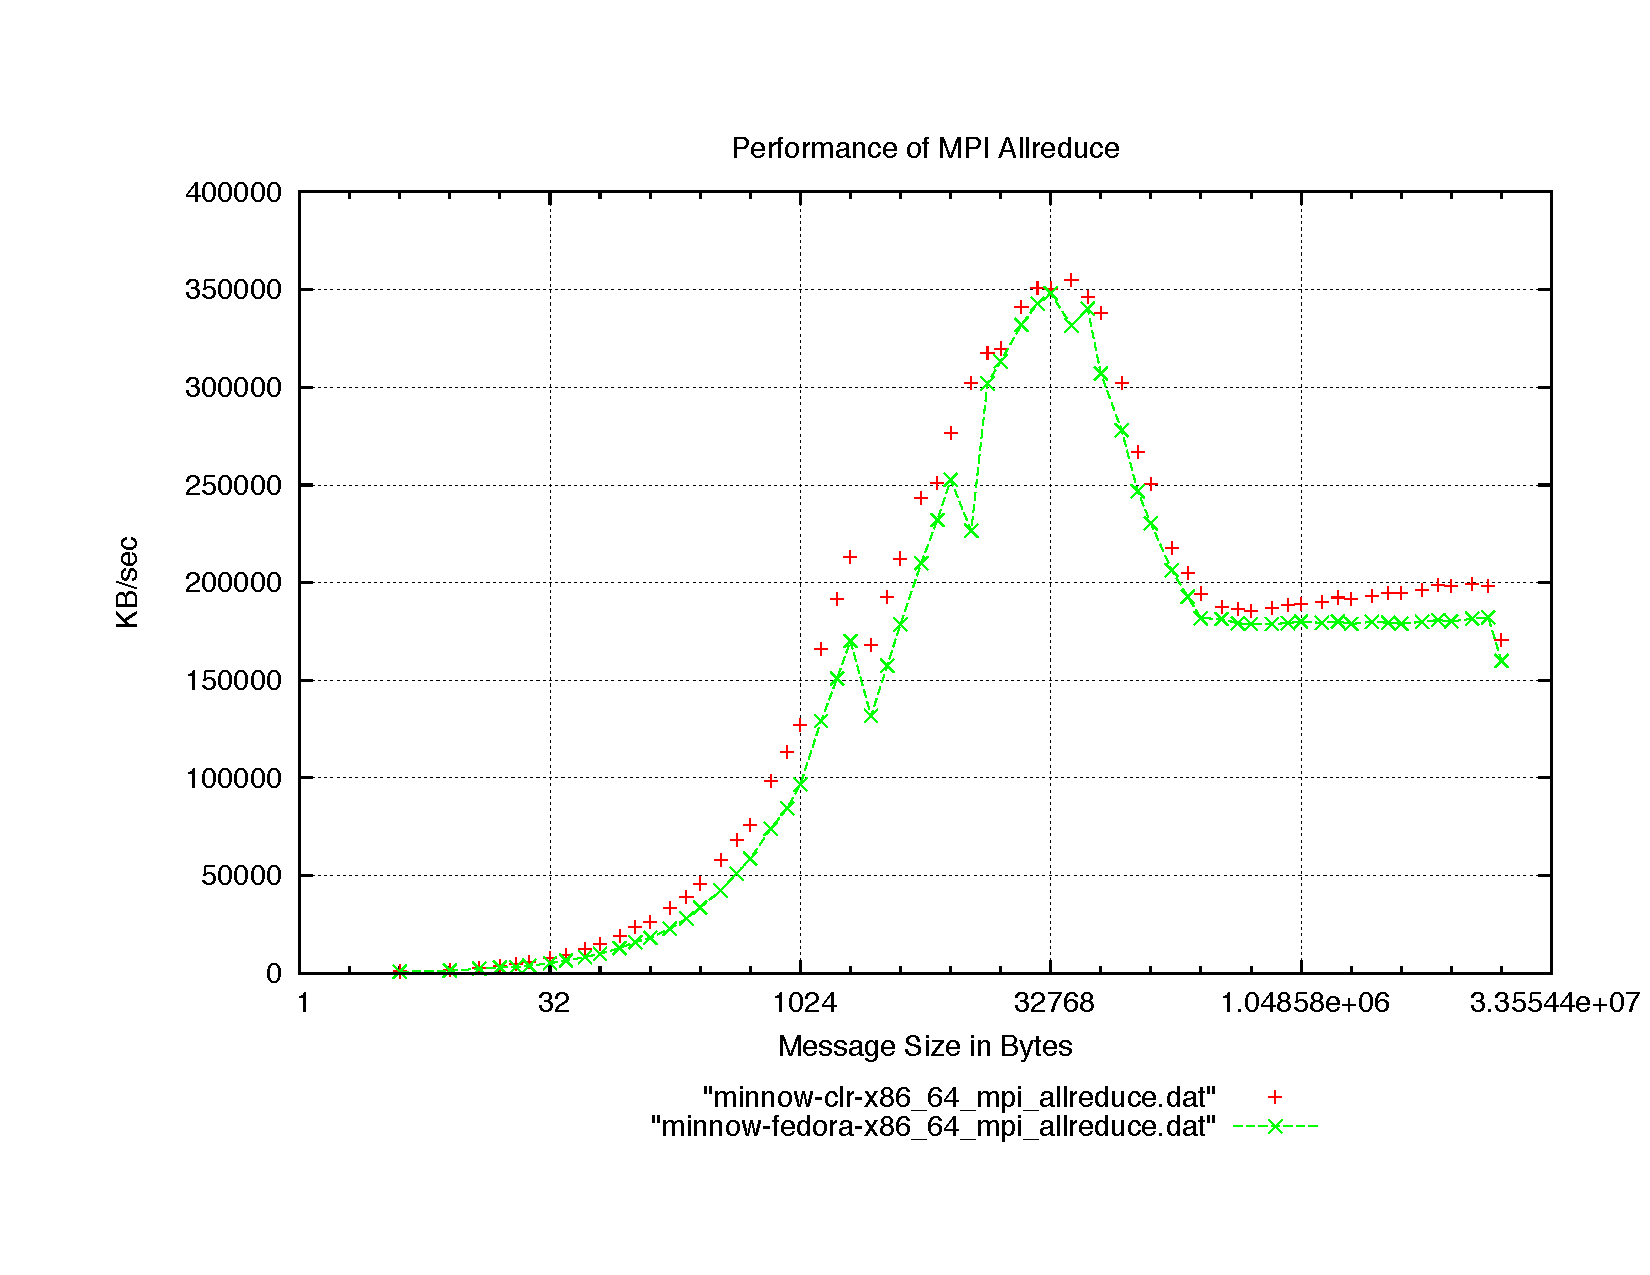
\includegraphics[width=0.75\textwidth]{images/mpbench_clr_experiments/mpi_allreduce.pdf}
\caption{MPI all reduce benchmark running in Minnowboard with Clear Linux and
Fedora (higher is better)}
\label{mpi_allreduce_clr_fedora}
\end{figure}

The all reduce benchmark (\ref{mpi_allreduce_clr_fedora}) shows more stable
performance running in a custom OS.  This can be seen in the drop of speed
(KB/sec) close to the test with a message size of 30000 Bytes. 

\begin{figure}[H]
\centering
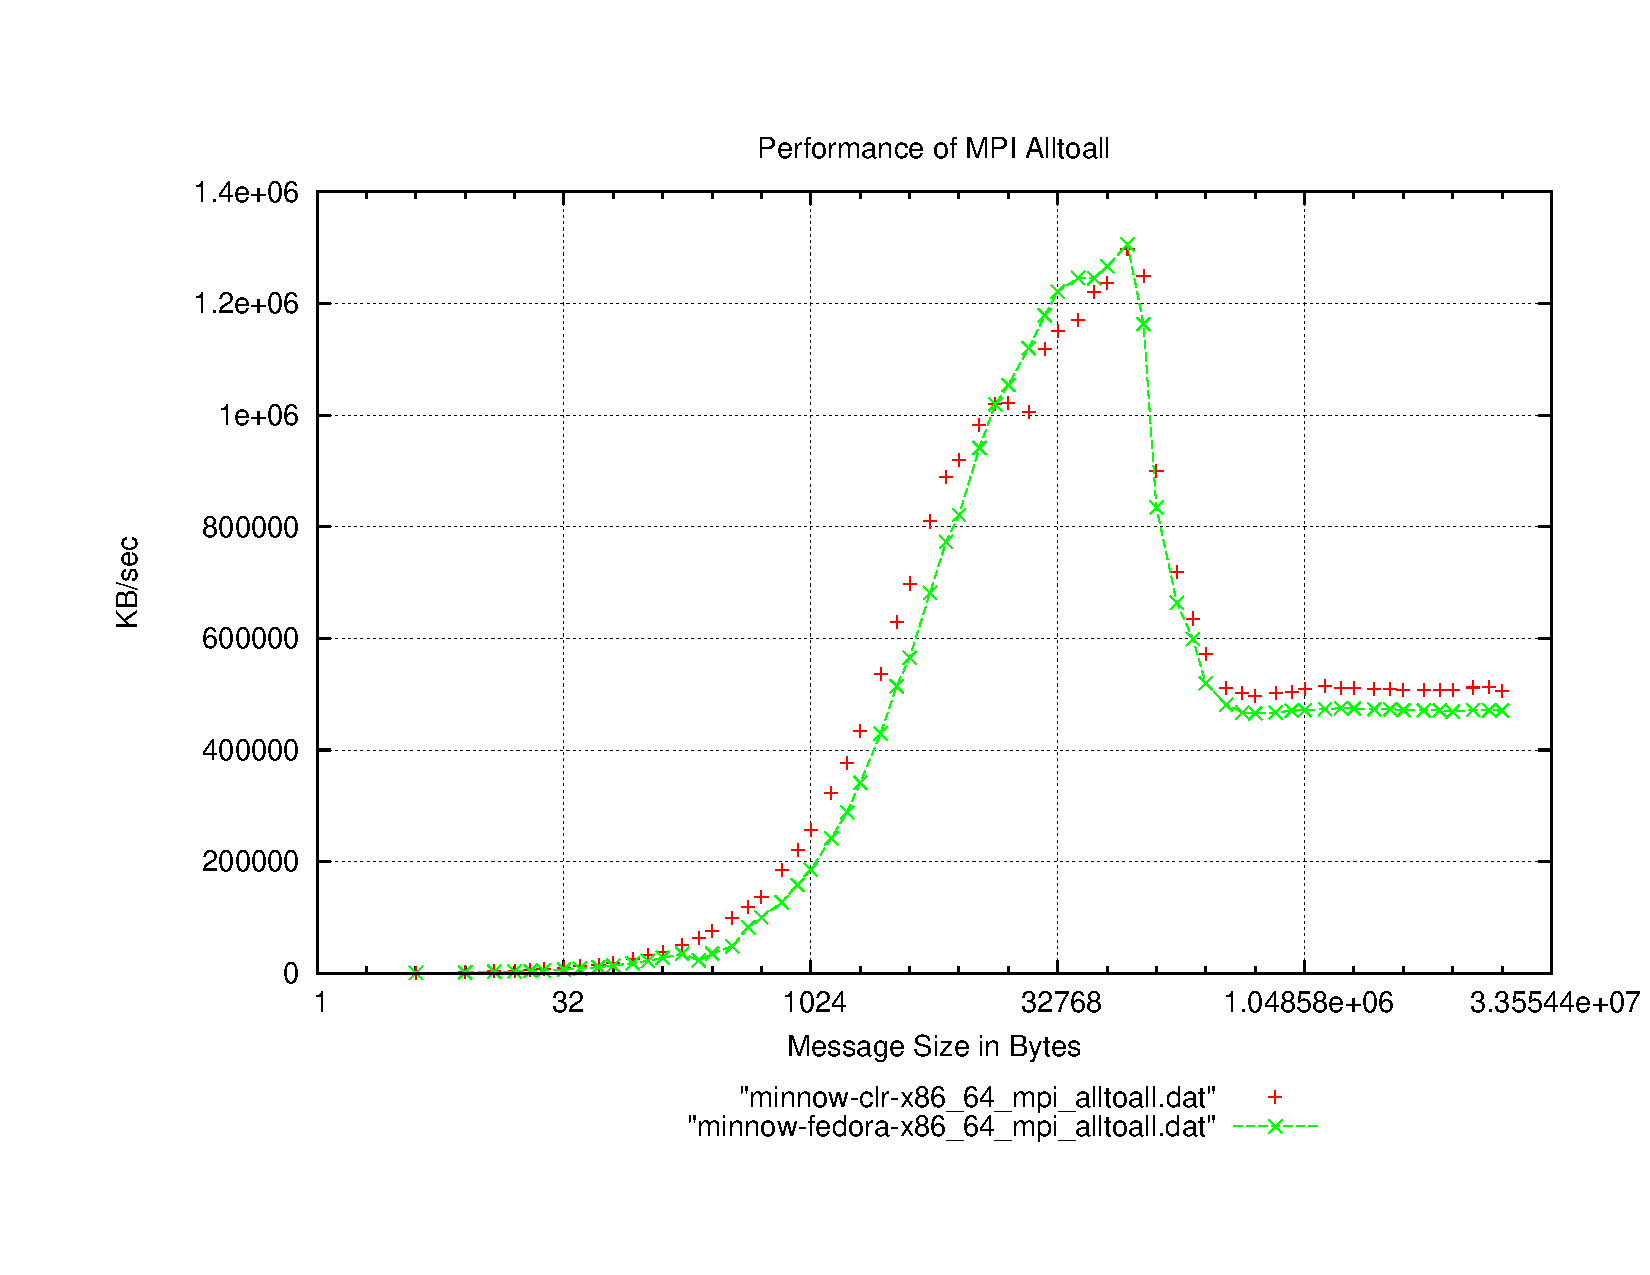
\includegraphics[width=0.75\textwidth]{images/mpbench_clr_experiments/mpi_alltoall.pdf}
\caption{MPI all to all benchmark running in Minnowboard with Clear Linux and
Fedora (higher is better)}
\label{mpi_alltoall_clr_fedora}
\end{figure}


\begin{figure}[H]
\centering
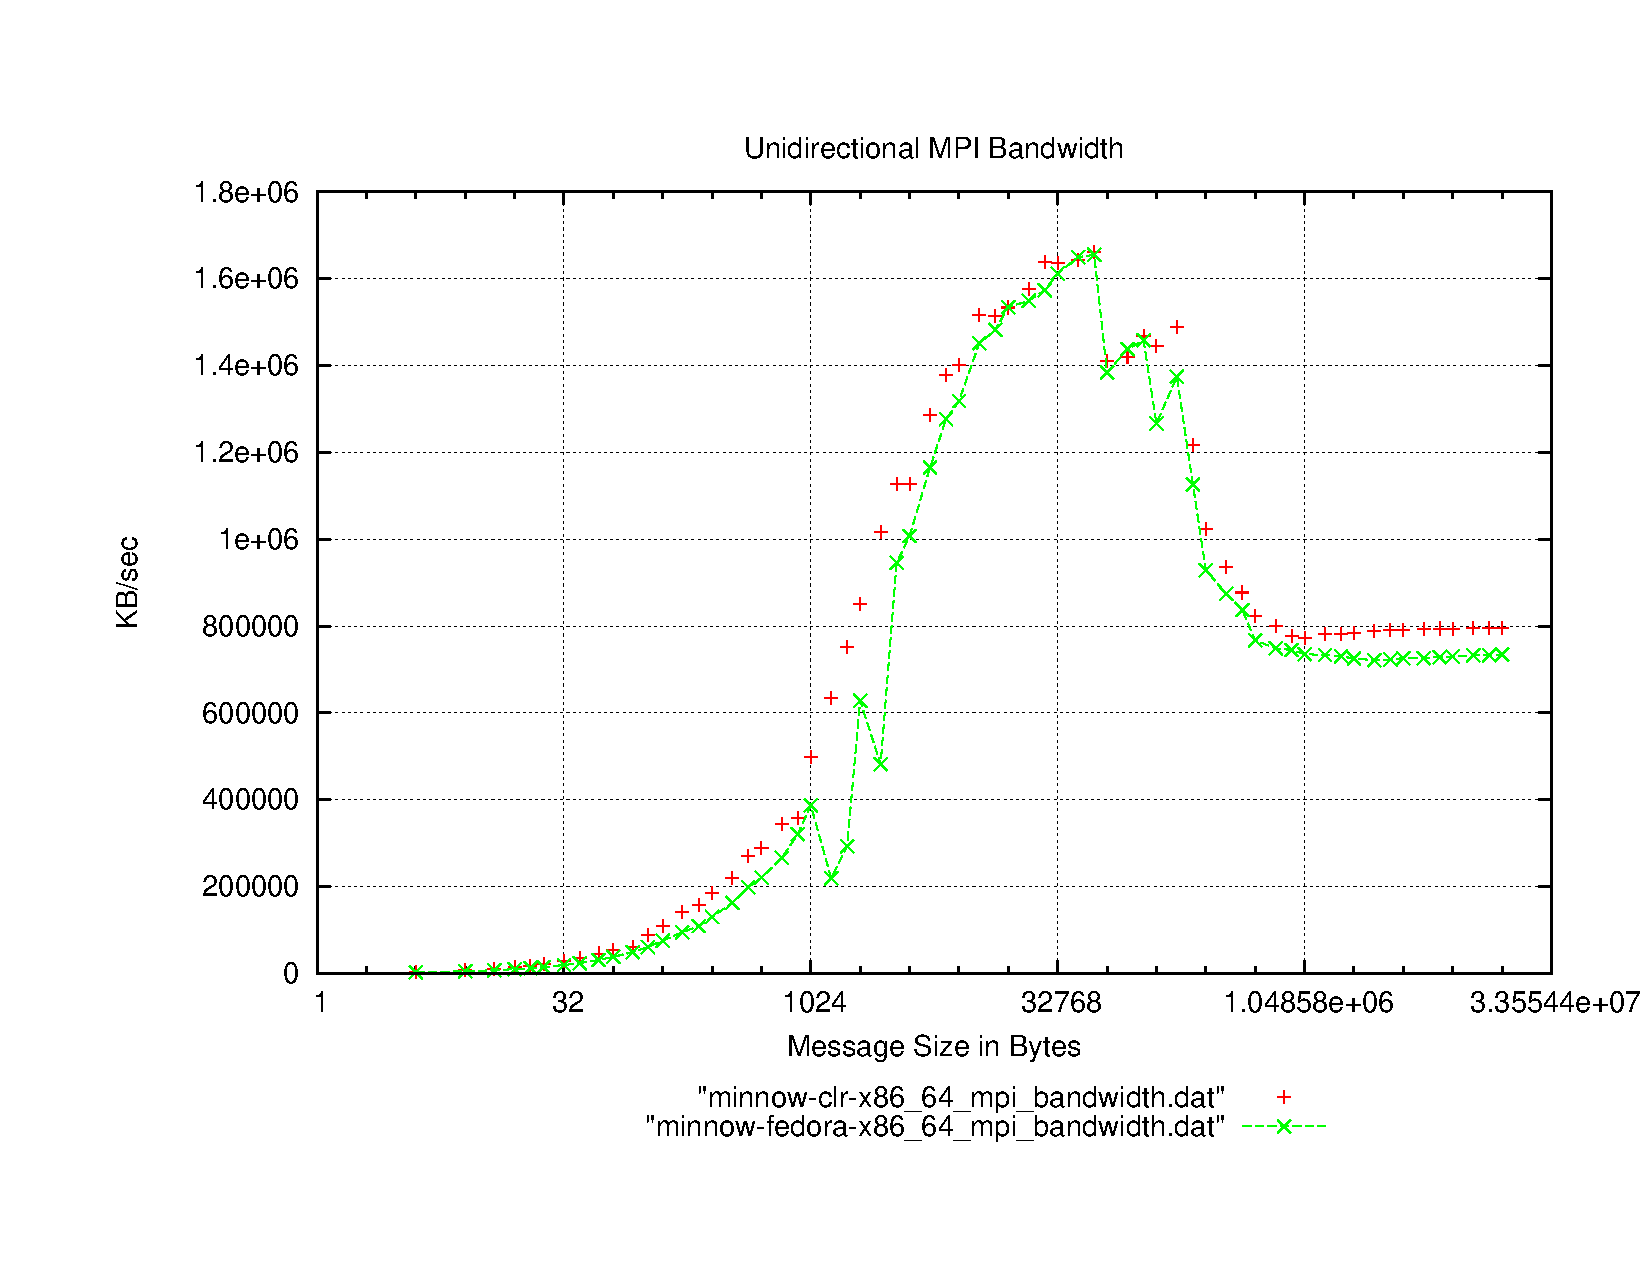
\includegraphics[width=0.75\textwidth]{images/mpbench_clr_experiments/mpi_bandwidth.pdf}
\caption{MPI bandwidth benchmark running in Minnowboard with Clear Linux and
Fedora (higher is better)}
\label{mpi_bandwidth_clr_fedora}
\end{figure}

The same results can bee seen in the "bandwidth" benchmark (figure
\ref{mpi_bandwidth_clr_fedora}); however in the "all to all" (figure
\ref{mpi_alltoall_clr_fedora}) there are no drops in speed at any size of the
message under test.  This is mainly because of the nature of the test , if we
remember both the "all reduce" and the "bandwidth" test execute the similar
tasks. Meanwhile bandwidth executes send and receives: 

\begin{lstlisting}[frame=single,numbers=left]
do over all message sizes 
    start timer
    do over iteration count 
        send(message size) 
        recv (4)
    stop timer
\end{lstlisting}

On the other hand mpi allreduce will reduce the values and distribute the
results to all processes. The function prototype is the following:

\begin{lstlisting}[frame=single,numbers=left]
MPI_Allreduce(
    void* send_data,
    void* recv_data,
    int count,
    MPI_Datatype datatype,
    MPI_Op op,
    MPI_Comm communicator)
\end{lstlisting}

MPI all reduce does the operation in each process and then broadcast the result
of the operation to all the individuals of the distributed system. This can be
seen in the figure \ref{mpi_allreduce_example}: 

\begin{figure}[H]
\centering
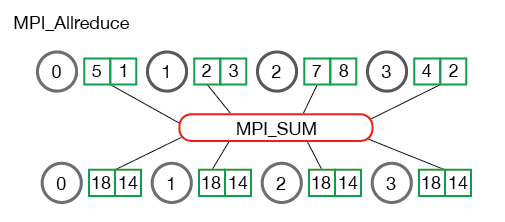
\includegraphics[width=0.75\textwidth]{images/mpi_allreduce_1.png}
\caption{MPI all reduce example }
\label{mpi_allreduce_example}
\end{figure}

As we can see both test exercise the send and receive functions of the OS. The
Clear Linux OS has specific implementations in the kernel that improve the
network performance, specially in the kernel network area

On the other hand the "all to all" sends data from all to all processes, this
mean that each node of the system need to send and receive data to every one.
This will mean an increase in the latency of the network. Another test just for
latency is executed in the future. 


\begin{figure}[H]
\centering
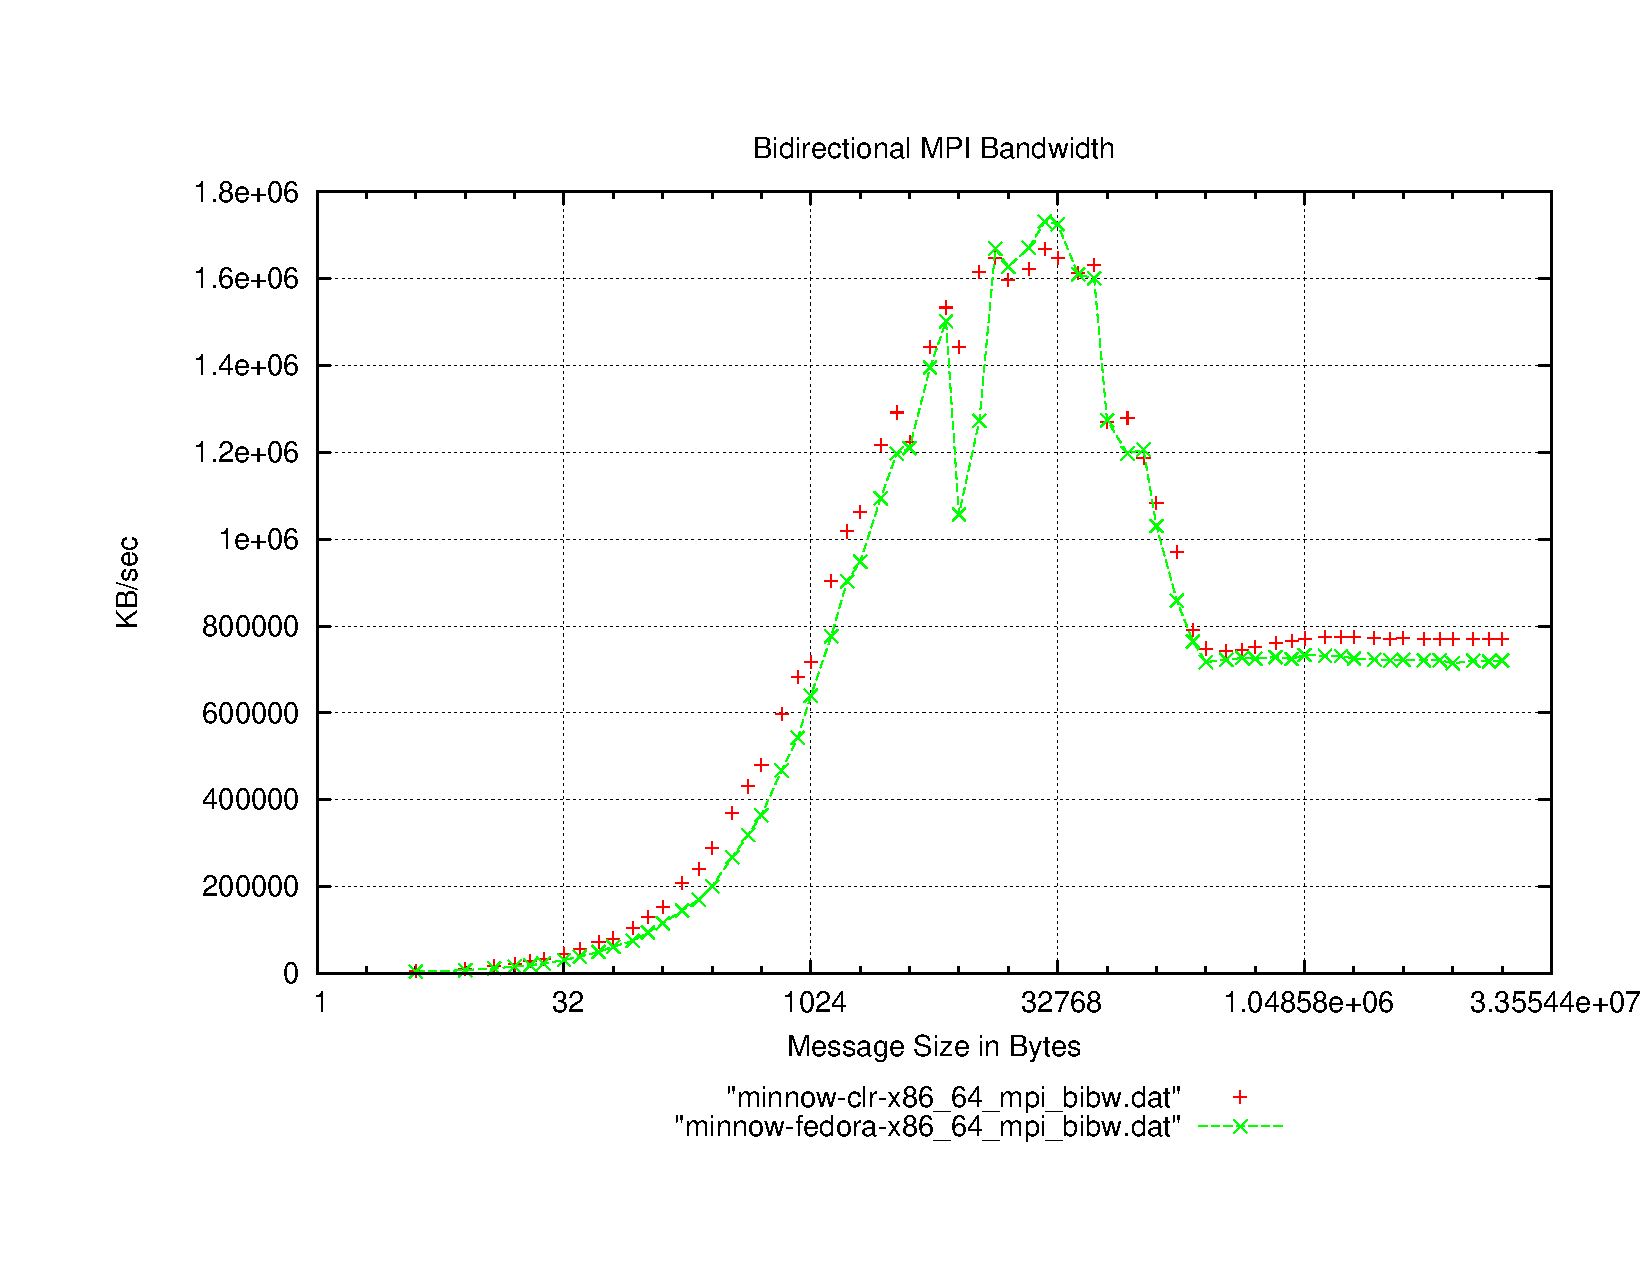
\includegraphics[width=0.75\textwidth]{images/mpbench_clr_experiments/mpi_bibw.pdf}
\caption{MPI Bi directional bandwidth running in Minnowboard with Clear Linux
and Fedora (higher is better)}
\label{mpi_bibw_clr_fedora}
\end{figure}


\begin{figure}[H]
\centering
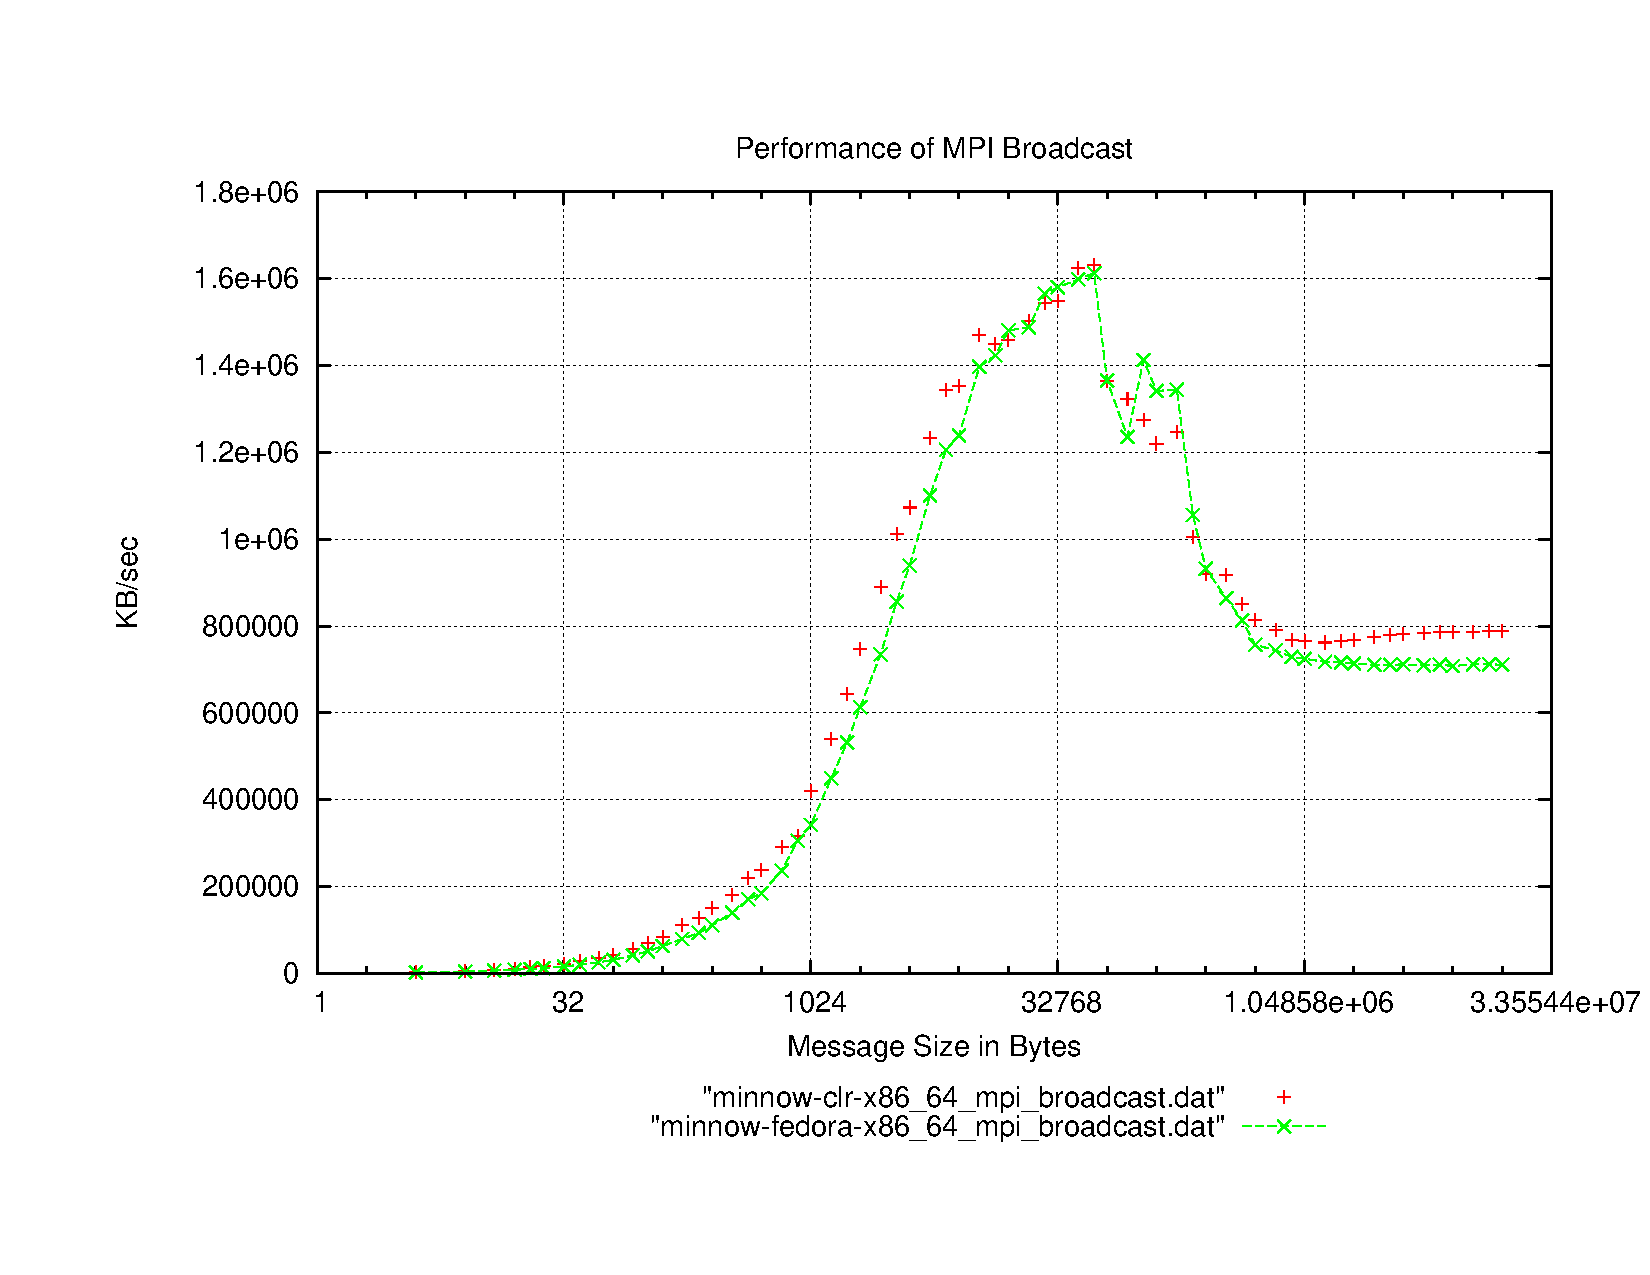
\includegraphics[width=0.75\textwidth]{images/mpbench_clr_experiments/mpi_broadcast.pdf}
\caption{MPI broadcast benchmark running in Minnowboard with Clear Linux and
Fedora (higher is better)}
\label{mpi_broadcast_clr_fedora}
\end{figure}

The same results can be sen in the bi directional bandwidth (figure
\ref{mpi_bibw_clr_fedora}) and the broadcast (figure
\ref{mpi_broadcast_clr_fedora}) test. As we remember the MPBench measures
bidirectional bandwidth with a doubly nested loop. The outer loop varies the
message size, and the inner loop measures the send operation over the iteration
count. Both processes execute a non-blocking receive, then a non-blocking send.
A non blocking send and receive mean that each process will release the
communication channel to other processes. If we check the number of processes
running in Fedora , the number is 30\% higher. This can bee seen in the figure
\ref{number_forks_fedora_clr}


\begin{figure}[H]
\centering
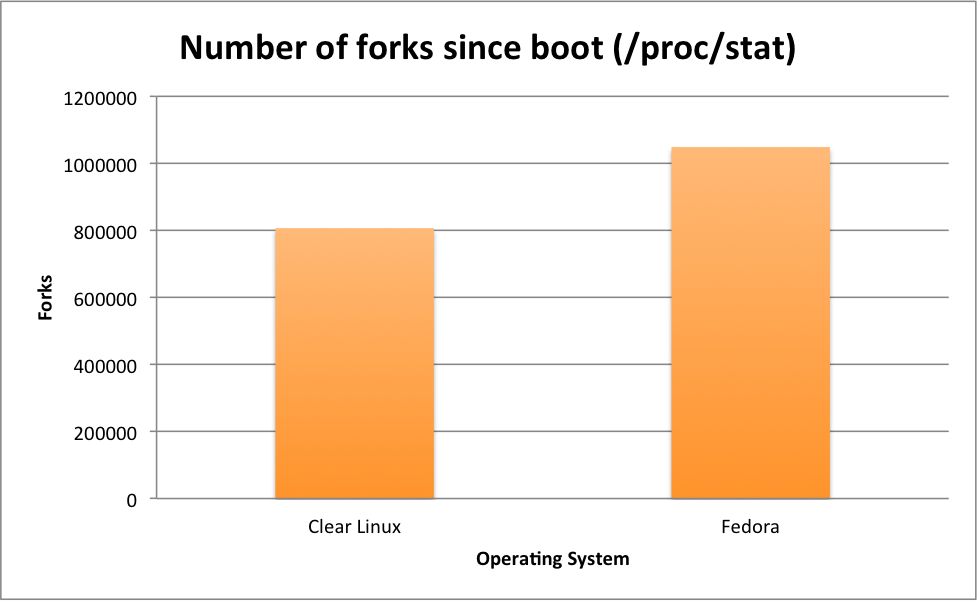
\includegraphics[width=0.75\textwidth]{images/number_forks.png}
\caption{Number of forks since boot reported in /proc/stat file (lower is better)}
\label{number_forks_fedora_clr}
\end{figure}

As we remember tin chapter 4 the latency benchmark can be described as one that
measures the time for an application to issue a send and continue computing.

The master's pseudo code for this test is as follows:

\begin{lstlisting}[frame=single,numbers=left]
do over all message sizes 
    start timer
    do over iteration count 
        send(message size) 
    stop timer
\end{lstlisting}    

The slaves' pseudo code is as follows:

\begin{lstlisting}[frame=single,numbers=left]
   do over all message sizes 
        start timer
        do over iteration count 
            recv(message size) 
        stop timer
\end{lstlisting}


As we can see in the figure \ref{mpi_latency_clr_fedora} there the latency in
both operating systems is pretty similar. The significant change is at the
beginning of the test (before the package size reach the 32 Bytes). This is due
to the fact that the test we are performing is with just 1 system, so there is
no network message does not have to travel among multiple points due to the
simplicity of our network (message send is received immediately) 

\begin{figure}[H]
\centering
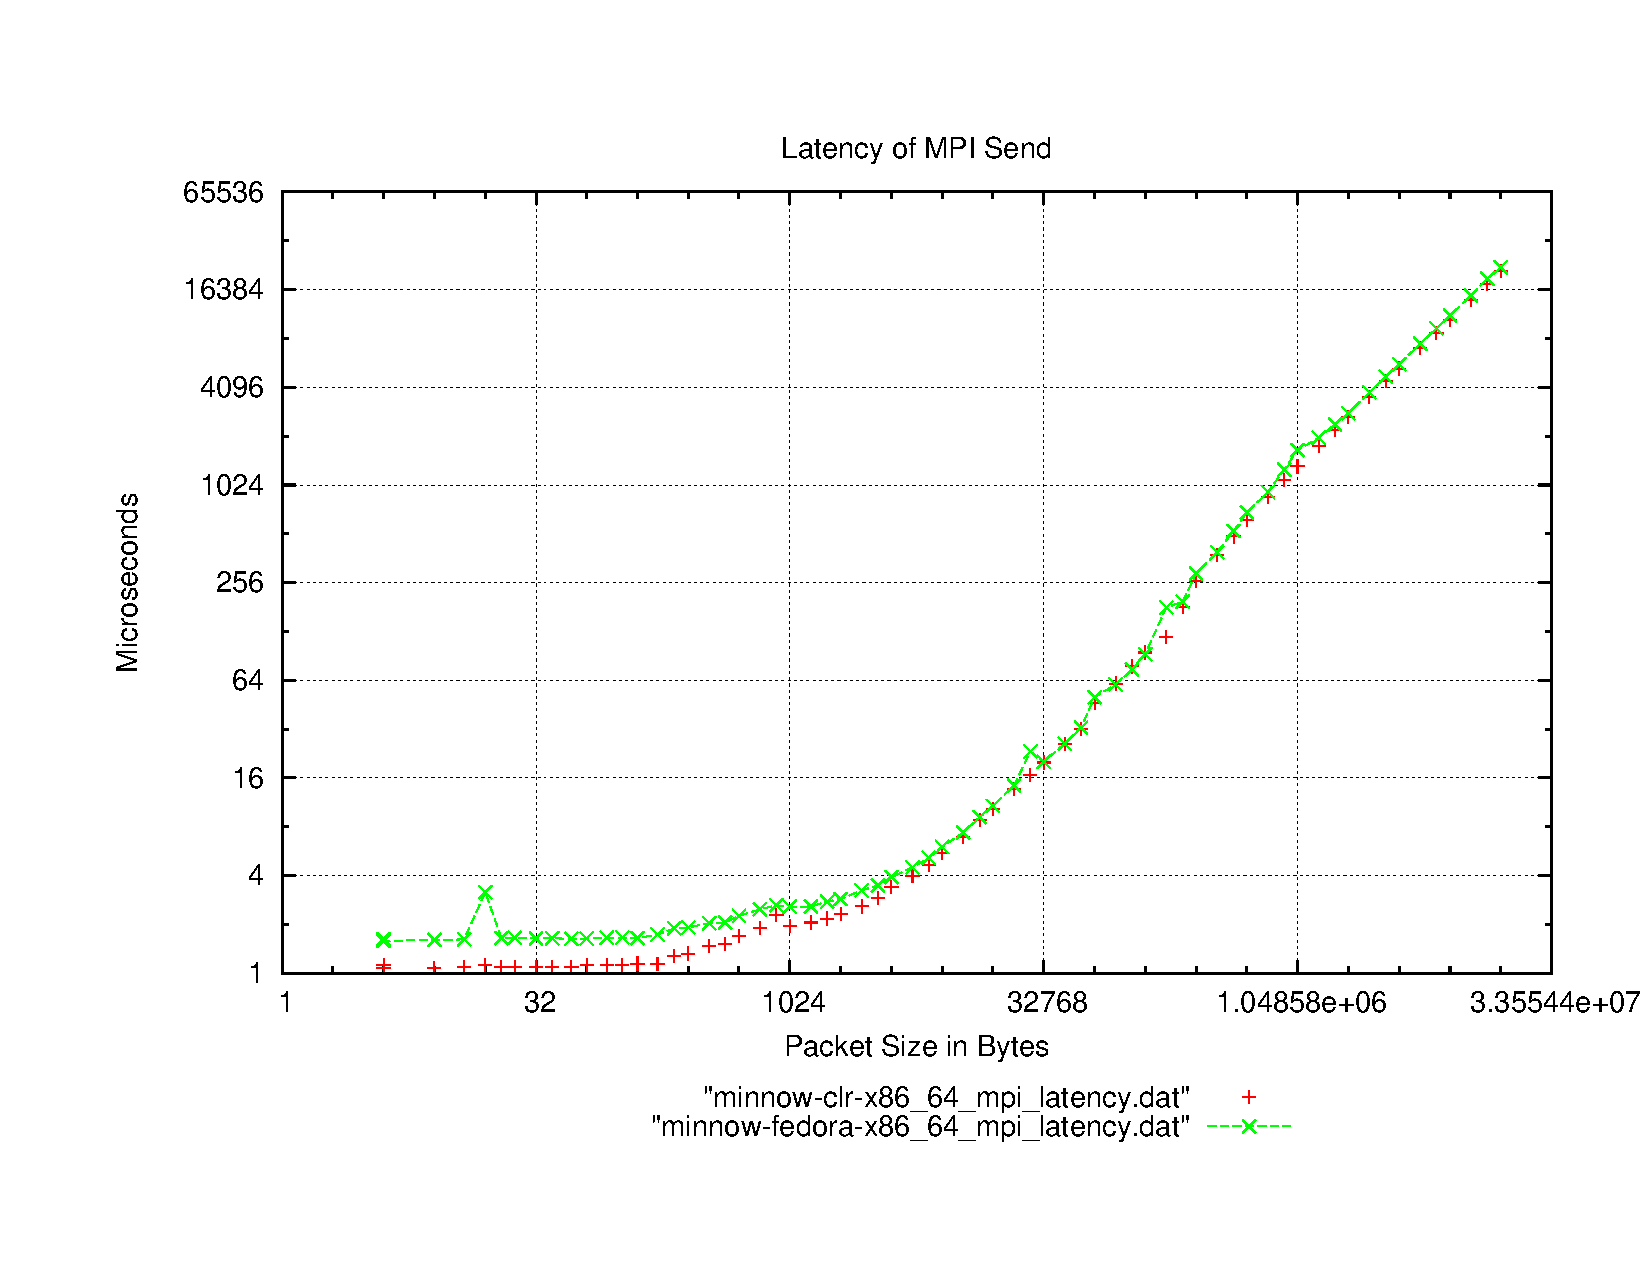
\includegraphics[width=0.75\textwidth]{images/mpbench_clr_experiments/mpi_latency.pdf}
\caption{MPI latency benchmark running in Minnowboard with Clear Linux and
Fedora (lower is better)}
\label{mpi_latency_clr_fedora}
\end{figure}



As we saw in chapter 4 roundtrip times are measured in much the same way as
bandwidth, except that, the slave process, after receiving the message, echoes
it back to the master.  This benchmark is often referred to as ping-pong. Here
our metric is transactions per second, which is a common metric for database
and server applications. No acknowledgment is needed with this test as it is
implicit given its semantics.

The master's pseudo code for this test is as follows:

\begin{lstlisting}[frame=single,numbers=left]
  do over all message sizes 
    start timer
    do over iteration count
        send(message size)
        recv(message size) 
        stop timer
\end{lstlisting}

The slaves' pseudo code is as follows:

\begin{lstlisting}[frame=single,numbers=left]
do over all message sizes 
    start timer
    do over iteration count
        recv(message size)
        send(message size)
    stop timer
\end{lstlisting}

We can see similar results in round trip test ( figure
\ref{mpi_roundtrip_clr_fedora} ) due to the same reasons in latency test. In
the future we will execute the same tests with up to 6 systems, there the
network results ( latency,roundtrip,bandwidth) might show different behaivor

\begin{figure}[H]
\centering
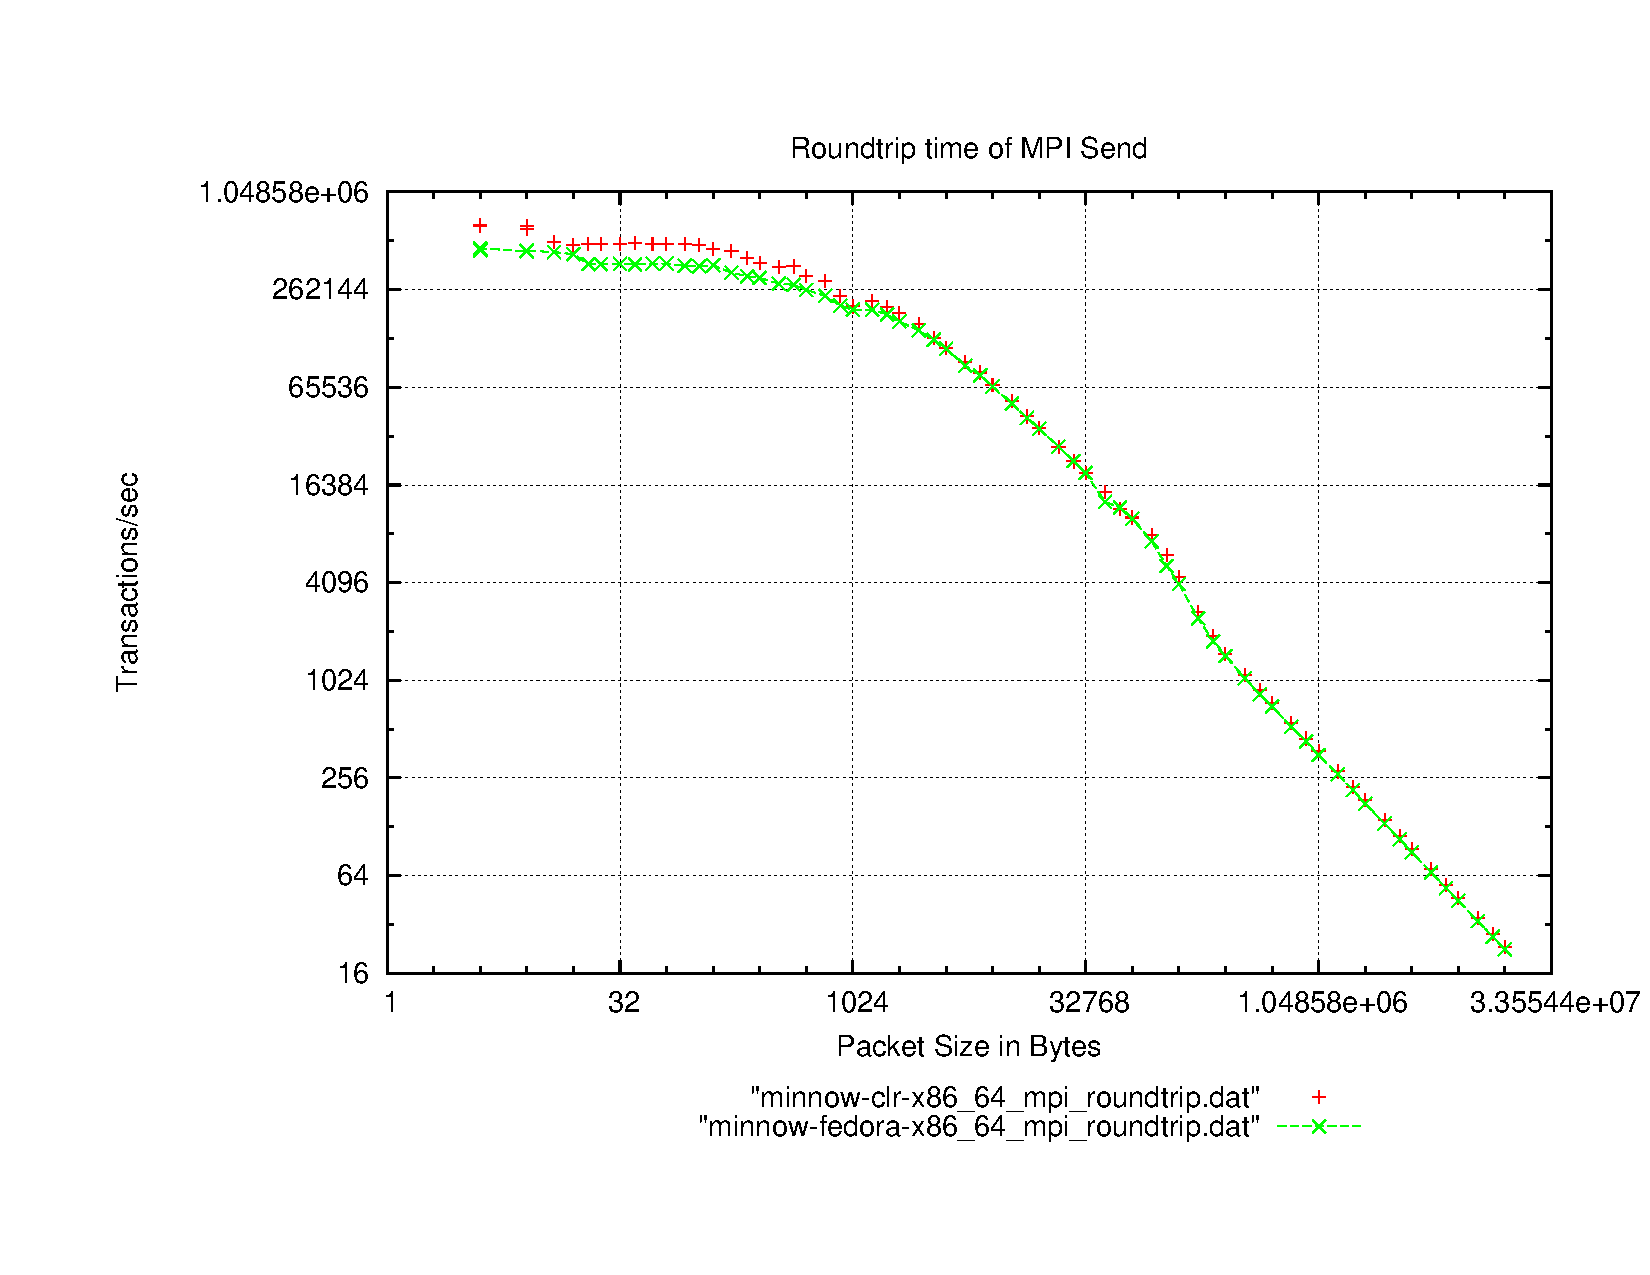
\includegraphics[width=0.75\textwidth]{images/mpbench_clr_experiments/mpi_roundtrip.pdf}
\caption{MPI latency benchmark running in Minnowboard with Clear Linux and
Fedora (lower is better)}
\label{mpi_roundtrip_clr_fedora}
\end{figure}

Based on the results we got from these experiments we came to the hypothesis
that a custom Operating System might represent a benefit for a cluster of
embedded platforms. We did the experiments with two operating systems , une
commercial ( Fedora ) and one custom (Clear linux for Intel Architecture). We
consider worth to try with an Operating System designed for Embedded and IoT
platforms. 

As we know the standard of the embedded industry to generate a custom Linux OS
is the Yocto project. As we saw in table~\ref{tab:4.2} the operating systems
generated with the Yocto project do not have an implementation of the MPI
library. 

If we want to repeat these experiments is necessary to make the MPI
implementation in the Yocto project. 


\section{Yocto project MPI implementation}

    \begin{center}
    \begin{tabular}{ | l | r |}
        \hline
        Platform under test & Minnow Board  Max \\ \hline
        Number of platforms  & 1  \\ \hline
        Operating System & Fedora / Clear Linux / Yocto base OS  \\ \hline
        SW to Test & MPI benchmark \\ \hline
    \end{tabular}
    \end{center}

The Yocto project \cite{yocto-project} generate a custom Linux OS for you
embedded system. The way you add a new capability to the system is by adding a
new receipt. This is described in the Yocto documentation. The receipt we
implemented for MPI is: 

\begin{lstlisting}[frame=single,numbers=left,breaklines=true,basicstyle=\tiny]

SUMMARY = "Message Passing Interface (MPI) implementation"
HOMEPAGE = "http://www.mpich.org/"
SECTION = "devel"

LICENSE = "BSD-2-Clause"
LIC_FILES_CHKSUM = "file://COPYRIGHT;md5=2106f0435056f3dd9349747a766e5816"

SRC_URI = " \
	http://www.mpich.org/static/downloads/${PV}/mpich-${PV}.tar.gz \
"

SRC_URI[md5sum] = "40dc408b1e03cc36d80209baaa2d32b7"
SRC_URI[sha256sum] = "455ccfaf4ec724d2cf5d8bff1f3d26a958ad196121e7ea26504fd3018757652d"

CACHED_CONFIGUREVARS += "BASH_SHELL=${base_bindir}/bash"

RDEPENDS_${PN} += "bash perl libxml2"
S = "${WORKDIR}/${BP}"

EXTRA_OECONF = "--enable-debuginfo \
                --enable-fast \
                --enable-shared  \
                --with-pm=gforker  \
		--disable-rpath \
                --disable-f77 \
                --disable-fc \
                --disable-fortran \
                --disable-cxx"

inherit autotools-brokensep gettext

do_configure_prepend() {
    autoreconf --verbose --install --force -I . -I confdb/ -I maint/
    oe_runconf
    exit
}

\end{lstlisting}

This receipt is part of the meta-openembedded layer, (
\url{http://cgit.openembedded.org/cgit.cgi/meta-openembedded/tree/meta-oe/recipes-devtools/mpich/mpich_3.1.1.bb?h=master})
a layer for all the embedded tools that the Linux distros mught need , in this
layer the user can add editors and other libraries that the embedded
application might need. 

The core of the MPI implementation we did is the configure part. Our configure
is described in the ''EXTRA\_OECONF''. The reasons why we did this are : 

\begin{itemize}
\item enable-debuginfo: For debugging the system when nedded
\item enable-fast Turns off error checking and collection of internal timing
information
\item enable-shared;Enable shared library support in order to split the MPI
capabilities in multiple binaries and shared object libraries . This makes the
compiler and process manager applications smaller in size.
\item with-pm=gforker:The gforker process manager is primiarily intended as a
debugging aid as it simplifies development and testing of MPI programs on a
single node or processor.
\item disable-rpath : Do not link to static libraries, if so the build
applications generated by this MPI implementations will not run in other MPI
system with different path of the libraries.
\item disable-f77:Build the Fortran 77 bindings (enabled by default).
\item disable-fc : Build the Fortran 90 bindings (enabled by default), since we
are not supporting Fortran we need to disable it 
\item disable-fortran: We need to disable fortran because Yocto project does
not suport Fortran
\item disable-cxx: Build the C++ bindings (enabled by default). We will not
support C++ in order to generate a small MPI implementation
\end{itemize}


\subsection{Results}

With this configuration we could create an MPI implementation in the Yocto
project, not just the compiler but also the MPI process manager. The results of
doin this can be seen in the following graphs of the MPI benchmarks, now
running with a Yocto base image: 

\begin{figure}[H]
\centering
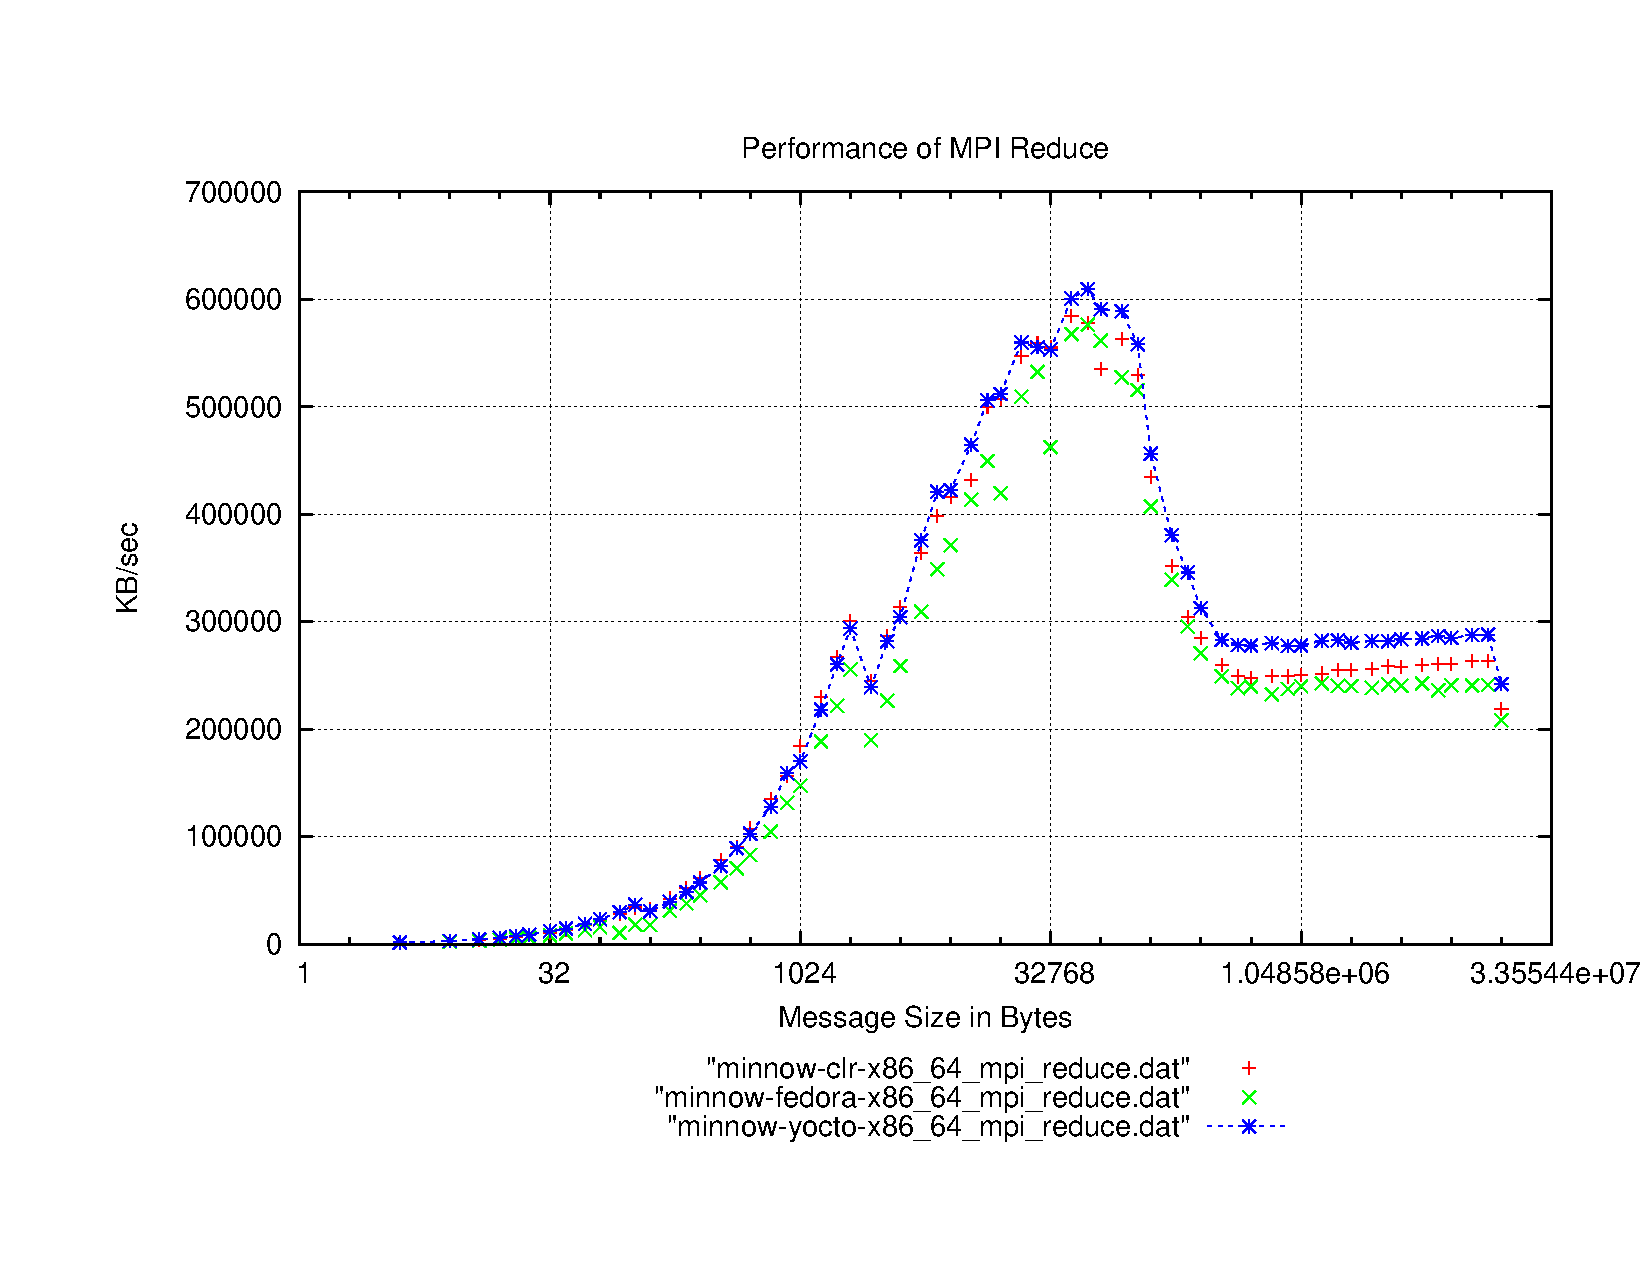
\includegraphics[width=0.75\textwidth]{images/mpbench_yocto_experiments/mpi_reduce.pdf}
\caption{MPI Reduce benchmark running in Minnowboard with Clear Linux, Yocto
and Fedora (higher is better)}
\label{mpi_reduce_yocto}
\end{figure}

\begin{figure}[H]
\centering
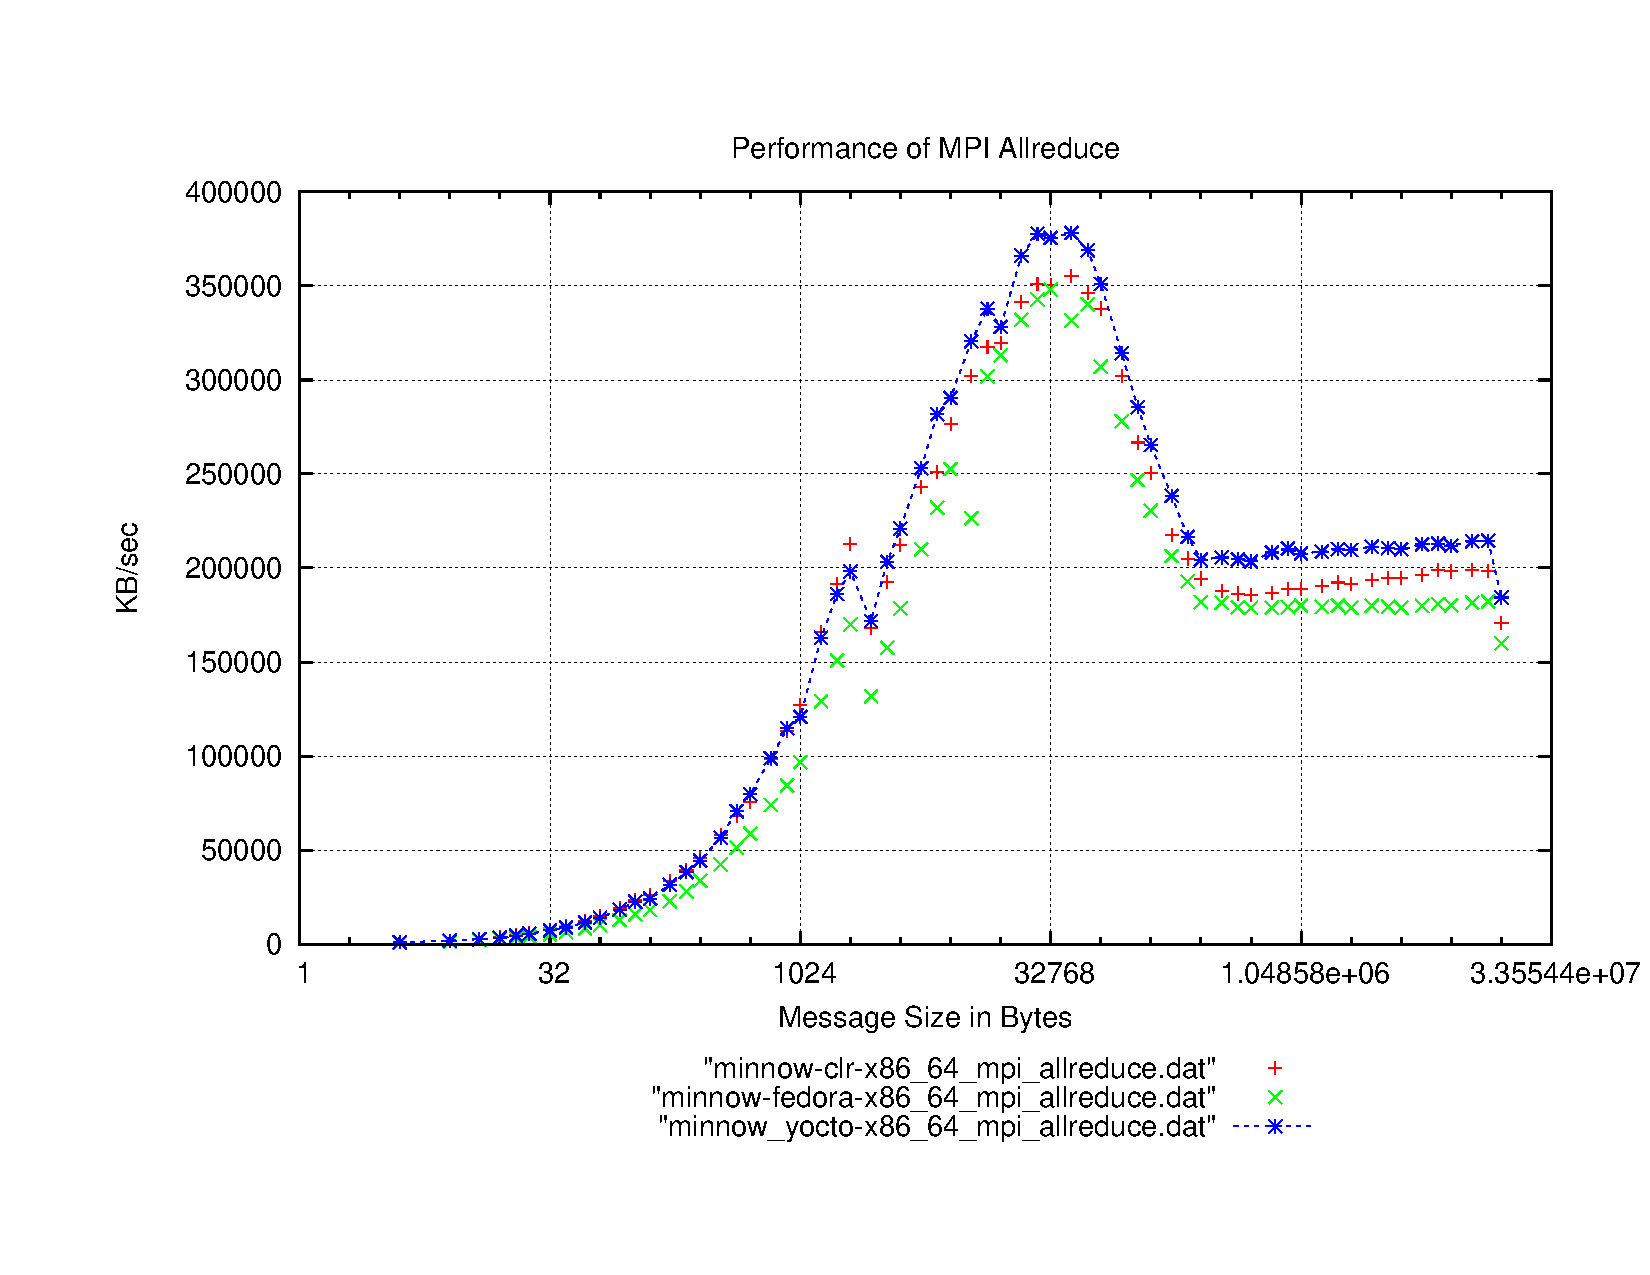
\includegraphics[width=0.75\textwidth]{images/mpbench_yocto_experiments/mpi_allreduce.pdf}
\caption{MPI all reduce benchmark running in Minnowboard with Clear Linux,
Yocto and Fedora (higher is better)}
\label{mpi_allreduce_yocto}
\end{figure}

\begin{figure}[H]
\centering
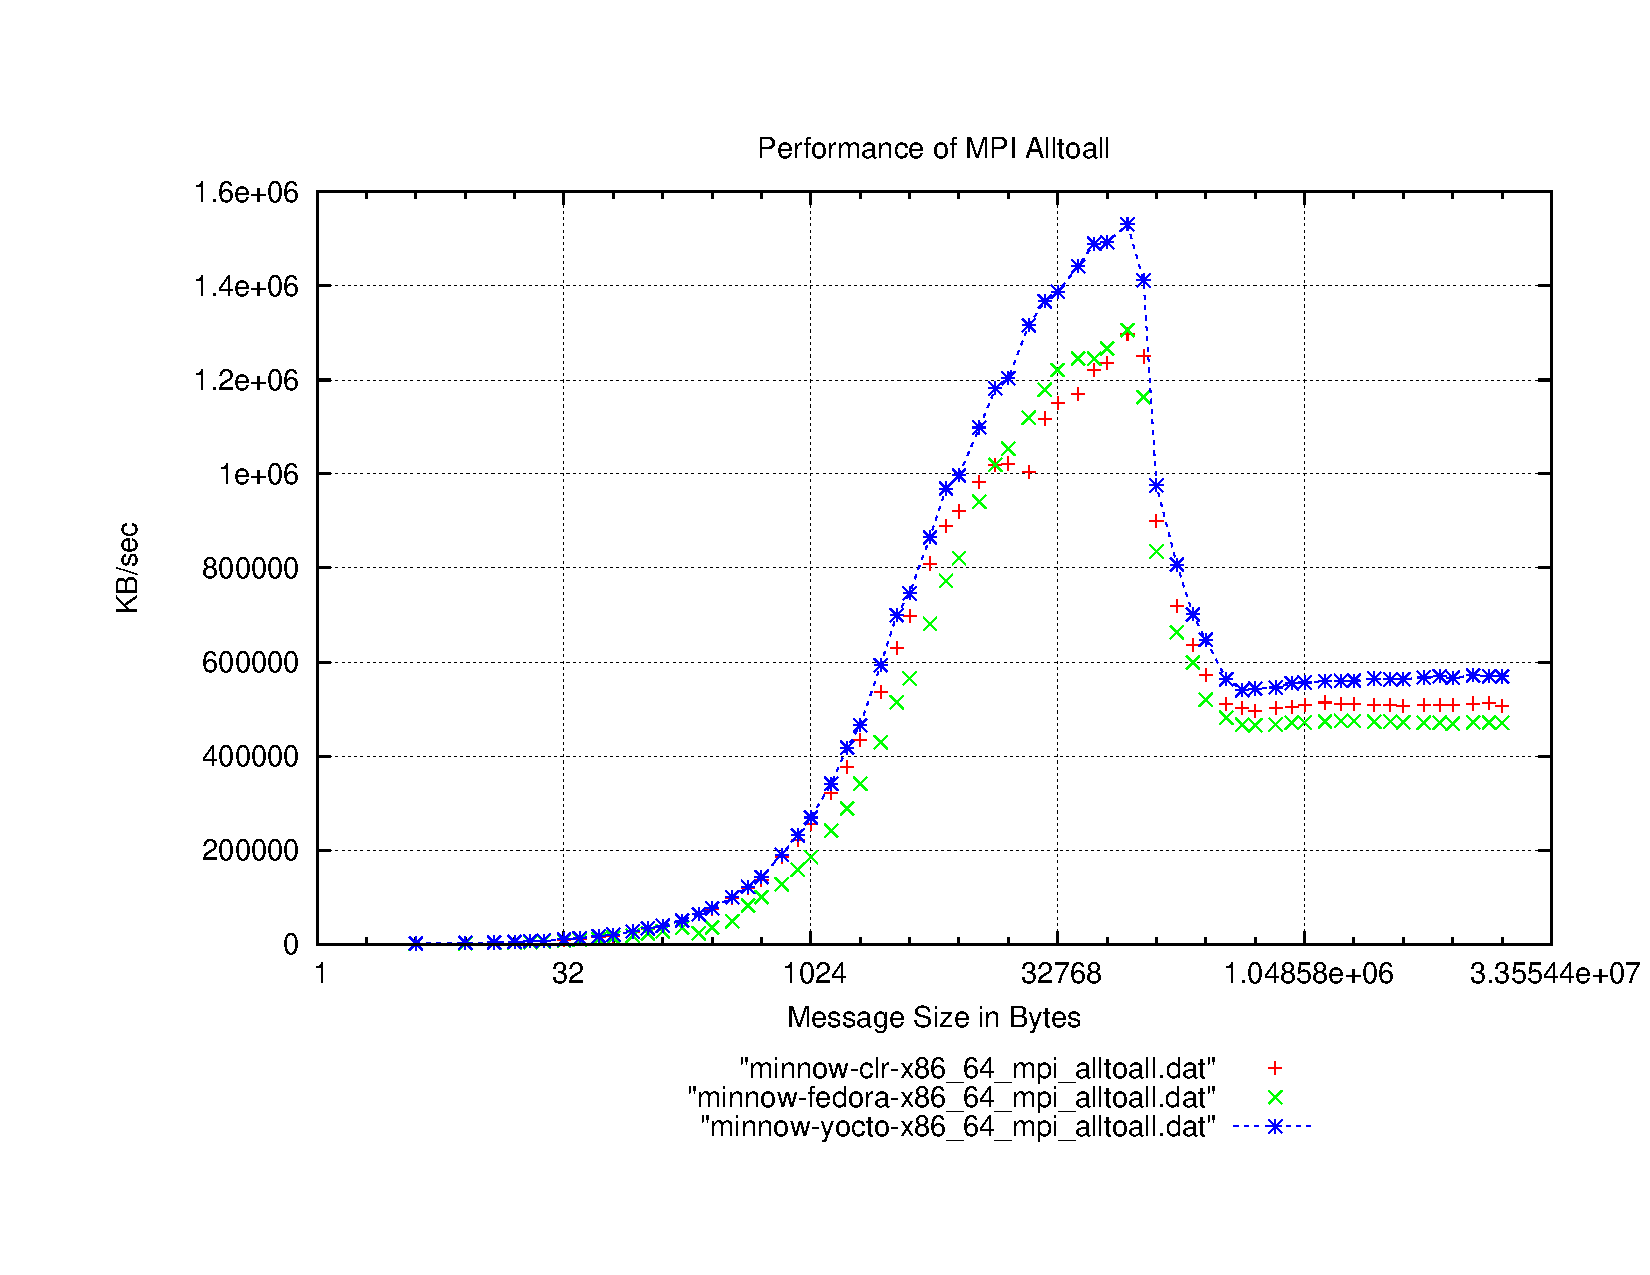
\includegraphics[width=0.75\textwidth]{images/mpbench_yocto_experiments/mpi_alltoall.pdf}
\caption{MPI all to all benchmark running in Minnowboard with Clear Linux, Yocto
and Fedora (higher is better)}
\label{mpi_all_to_all_yocto}
\end{figure}

As we can see the results with the Yocto base operating system have the same
tendency that with the Clear Linux base OS. Except in the "all to all"
experiment where the gain in performance was higher with a message size higher
than 32000 Bytes. This is pretty much because of the nature of the test. As we
remember the test measures a kind of round-robin communication among multiple
processes.

\begin{lstlisting}[frame=single,numbers=left]
    do over all message sizes 
        start timer
        do over iteration count 
            all-to-all(message size)
        stop timer
\end{lstlisting}

The all to all systems is described in figure \ref{mpi_all_to_all_example}.
MPI all to all  is a collective operation in which all processes send the same
amount of data to each other, and receive the same amount of data from each
other. As we can see on the figure each process has its own data , at the end,
all the processes has the same amount of data from each one. In the figure we
can see how each process distribute its data among the other processes.

\begin{figure}[H]
\centering
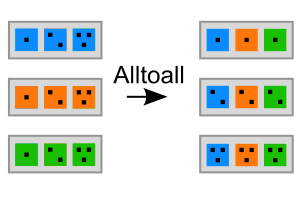
\includegraphics[width=0.75\textwidth]{images/mpi_all_to_all.png}
\caption{MPI all to all mechanism diagram}
\label{mpi_all_to_all_example}
\end{figure}

Each of these process are blocking processes, which mean that the number of
processes does not affect the performance of the test. However when we check
the configuration of the Yocto Base operating system we can see there there
some modifications for the specific platform we are testing. Specially in the
kernel section: 

\begin{lstlisting}[frame=single,numbers=left]
    # enable cpu frequency scaling and stats for powertop
    CONFIG_CPU_FREQ=y
    CONFIG_CPU_FREQ_STAT=y
    CONFIG_X86_ACPI_CPUFREQ=y
    CONFIG_X86_INTEL_PSTATE=y
    CONFIG_CPU_FREQ_GOV_ONDEMAND=y
    CONFIG_CPU_FREQ_GOV_PERFORMANCE=y
    CONFIG_CPU_FREQ_DEFAULT_GOV_ONDEMAND=y
\end{lstlisting}

The Yocto kernel for the platform under test ( Minnow Board Max ) has the CPU
frequency scaling enable. Clock scaling allows you to change the clock speed of
CPUs on the fly. This is a nice method to save battery during runtime as well
as a nice method to boos the speed of the system when required. In this case
the speed of the system is increased upon request when send/receive method
require it.

\begin{figure}[H]
\centering
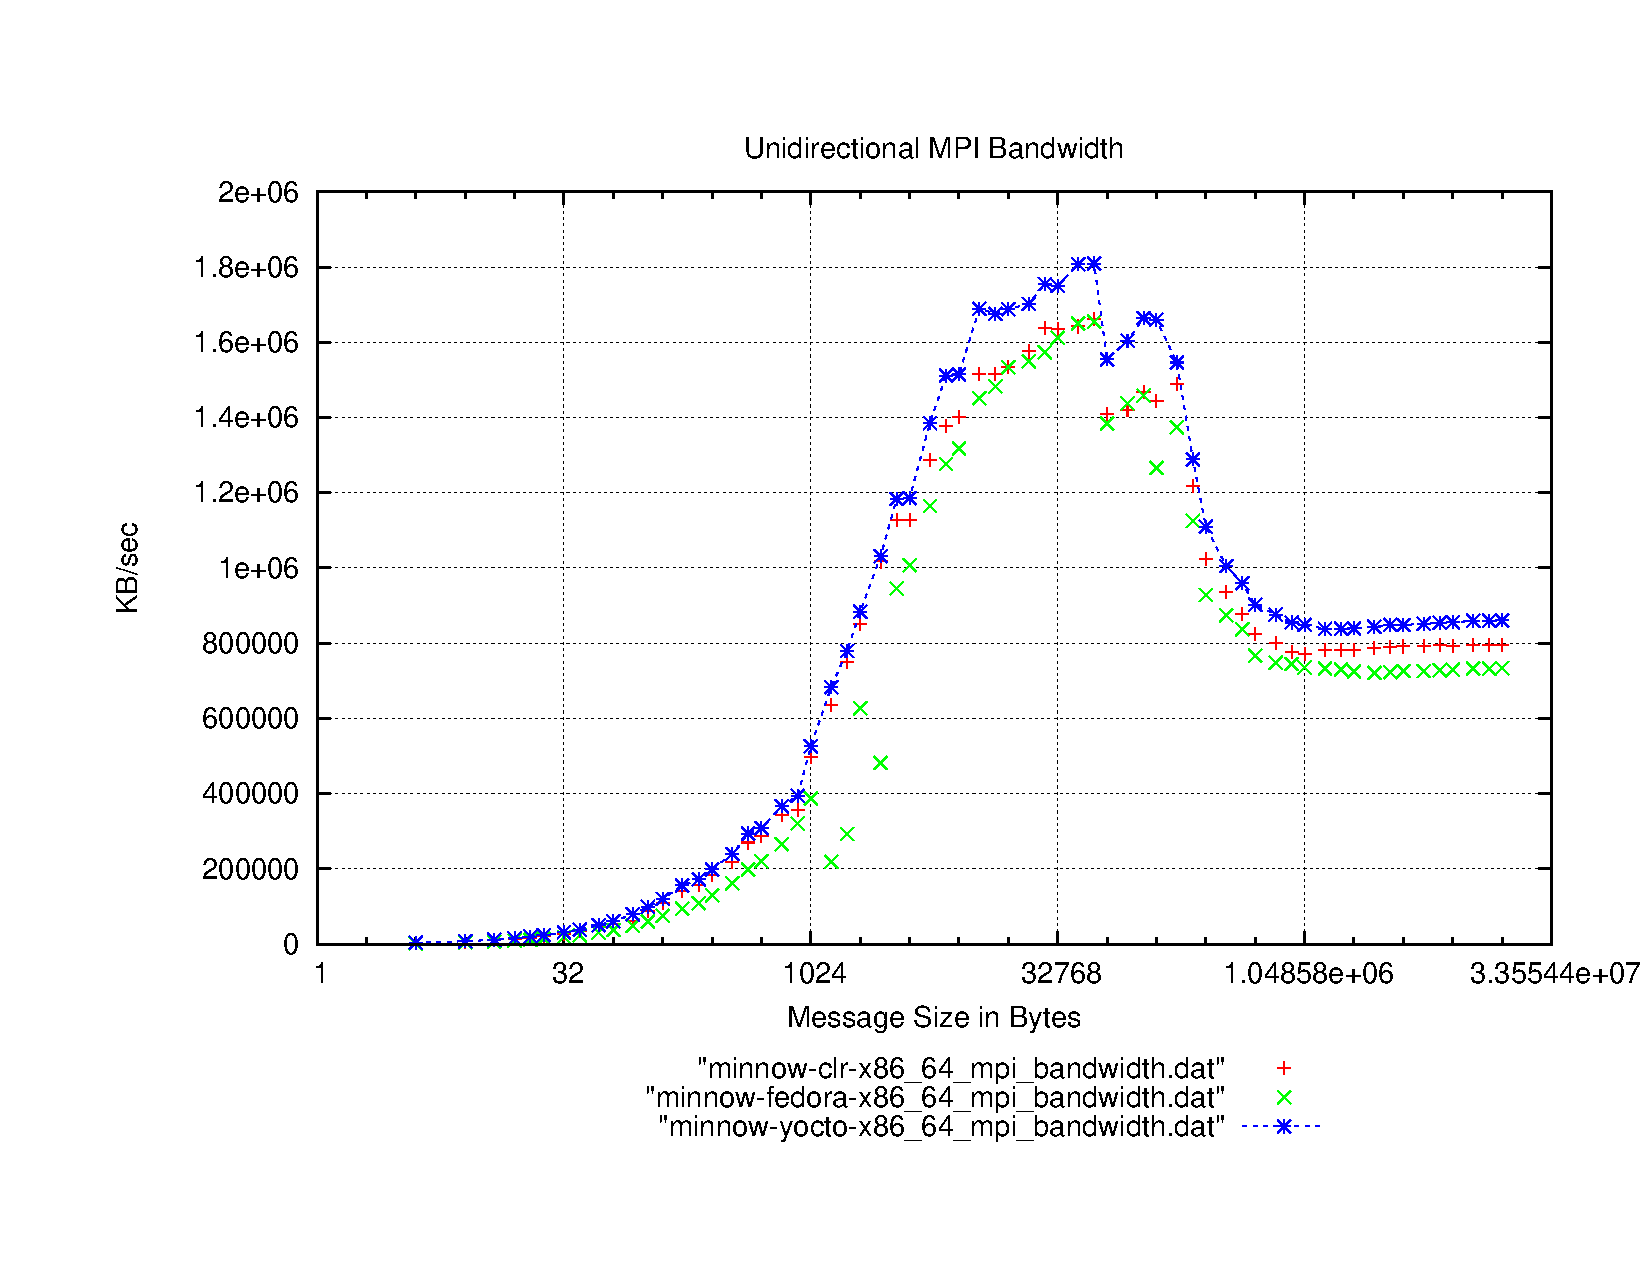
\includegraphics[width=0.75\textwidth]{images/mpbench_yocto_experiments/mpi_bandwidth.pdf}
\caption{MPI bandwidth benchmark running in Minnowboard with Clear Linux,
Yocto and Fedora (higher is better)}
\label{mpi_bandwidth_yocto}
\end{figure}


\begin{figure}[H]
\centering
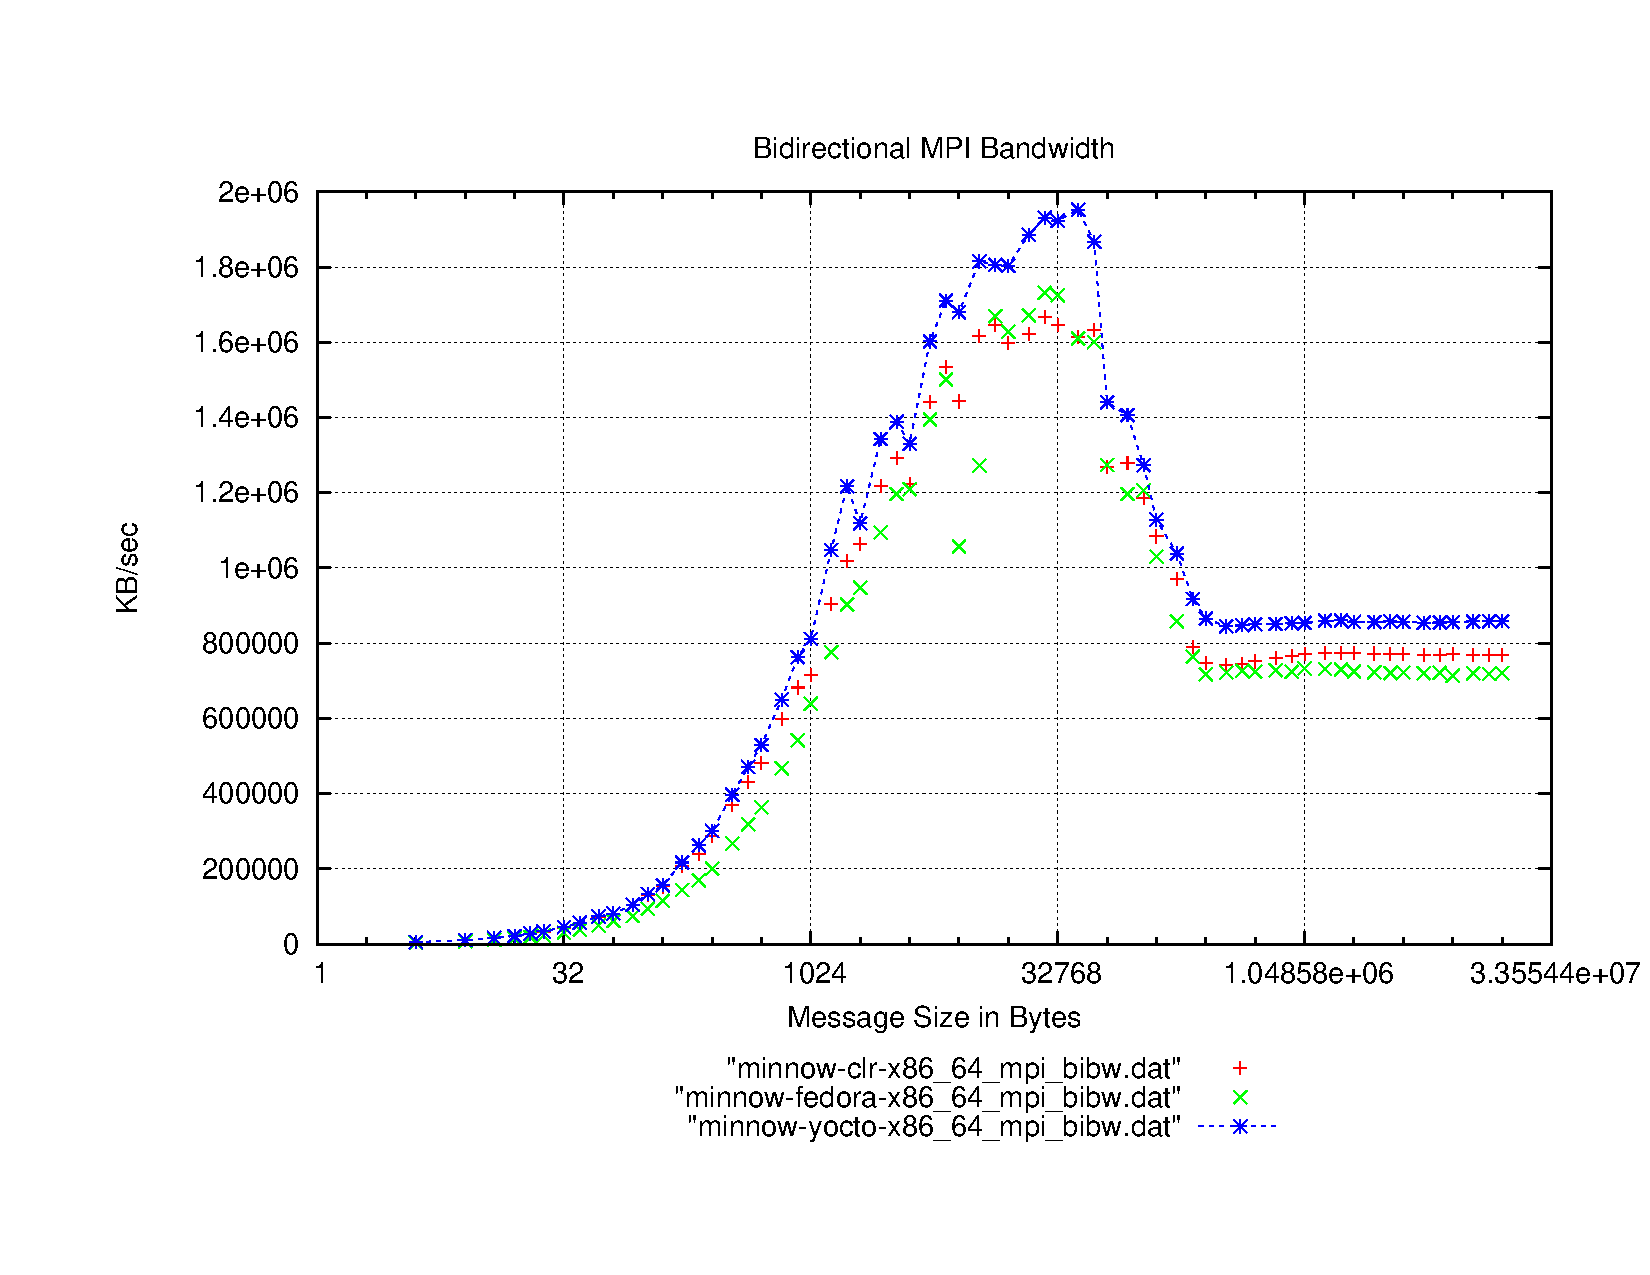
\includegraphics[width=0.75\textwidth]{images/mpbench_yocto_experiments/mpi_bibw.pdf}
\caption{MPI Bi directional bandwidth running in Minnowboard with Clear Linux,
Yocto and Fedora (higher is better)}
\label{mpi_bibw_yocto}
\end{figure}


\begin{figure}[H]
\centering
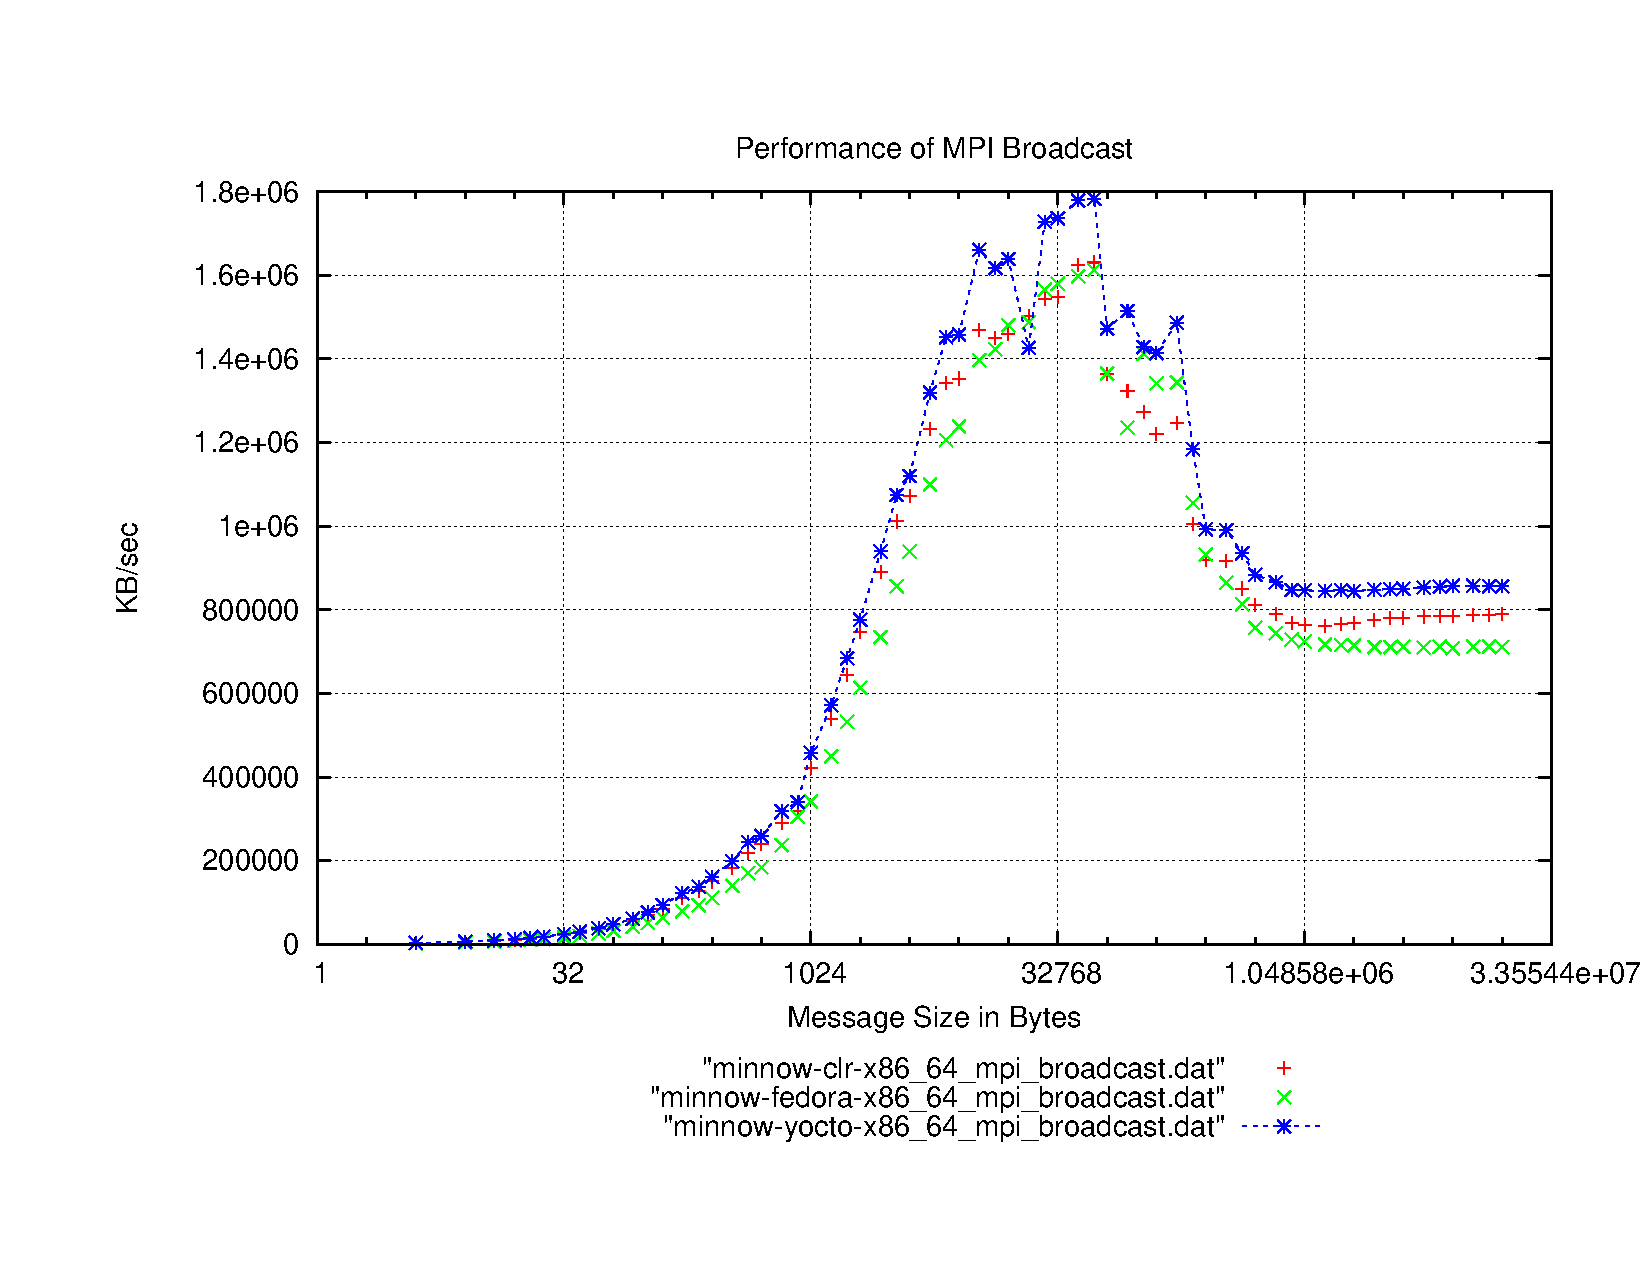
\includegraphics[width=0.75\textwidth]{images/mpbench_yocto_experiments/mpi_broadcast.pdf}
\caption{MPI Broadcast benchmark running in Minnowboard with Clear Linux, Yocto
and Fedora (lower is better)}
\label{mpi_broadcast_yocto}
\end{figure}

If we remember the results we got in the previous tests of bi directional band
width (figure \ref{mpi_bibw_clr_fedora}) and the broadcast test (figure
\ref{mpi_broadcast_clr_fedora}) , the main reason why Clear Linux ran with
higher speed was because of the number of processes (forks) since fighting for
the same resources ( network / memory / CPU) . Now if we check the number of
processes running in Yocto base OS , the number is 15\% lower than CLR and 35\%
lower than Fedora . This can bee seen in the figure \ref{number_forks_yocto}

\begin{figure}[H]
\centering
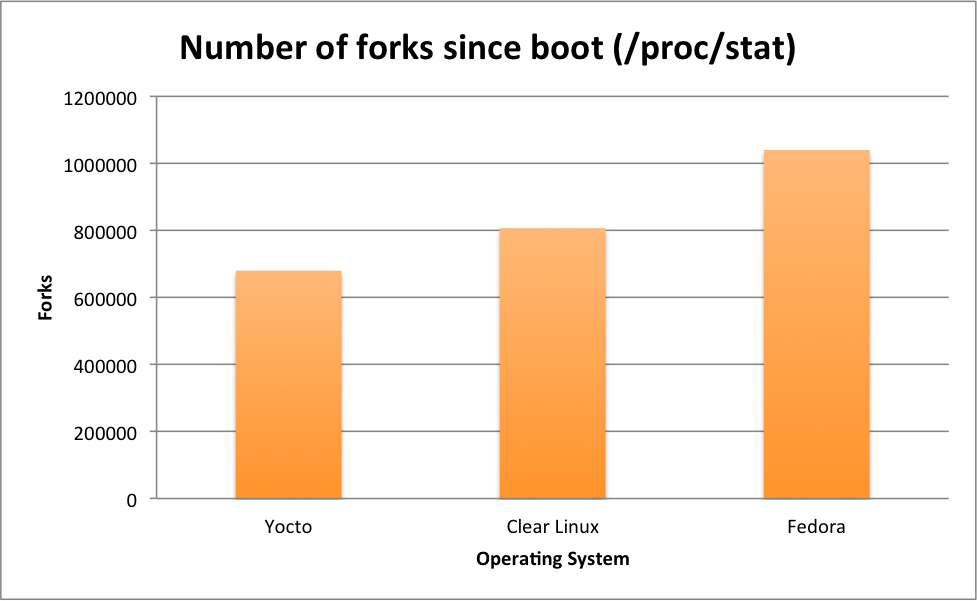
\includegraphics[width=0.75\textwidth]{images/number_forks_yocto.png}
\caption{Number of forks since boot reported in /proc/stat file (lower is better)}
\label{number_forks_yocto}
\end{figure}

\begin{figure}[H]
\centering
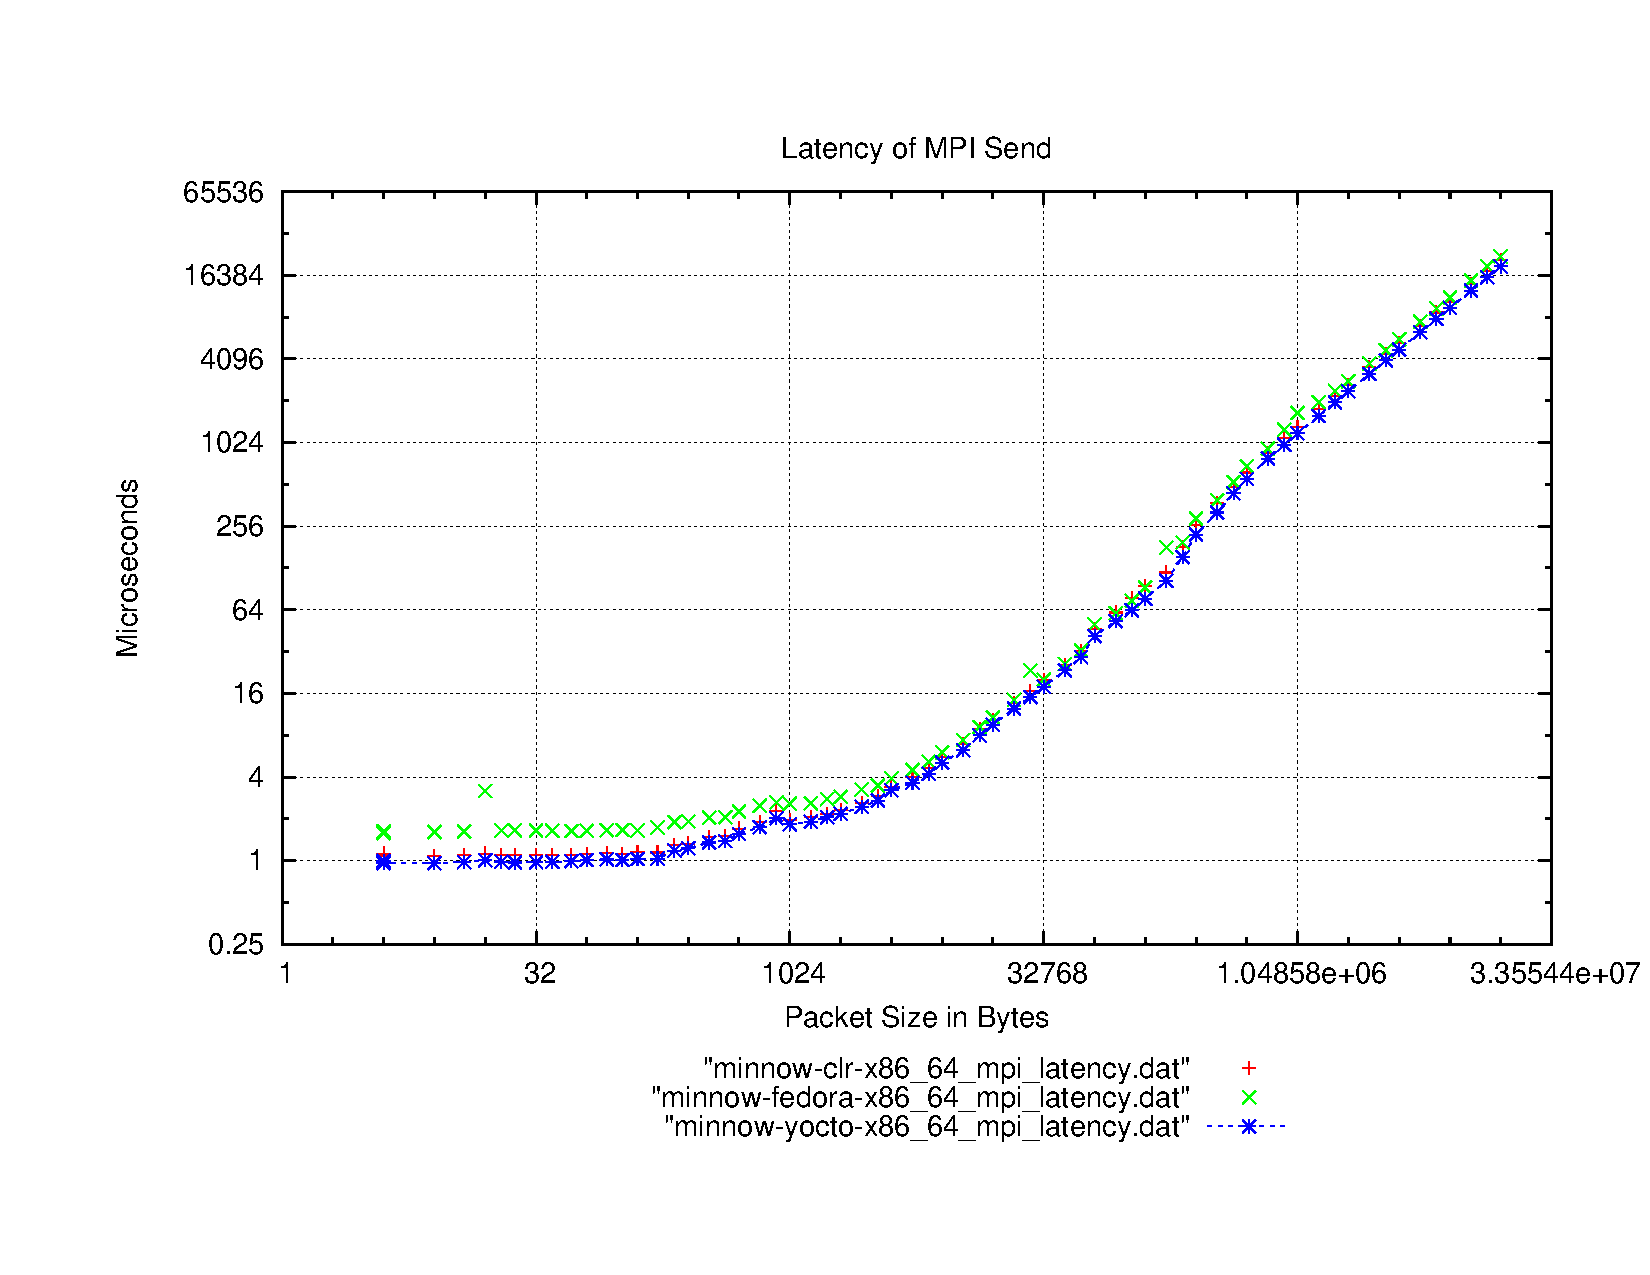
\includegraphics[width=0.75\textwidth]{images/mpbench_yocto_experiments/mpi_latency.pdf}
\caption{MPI latency running in Minnowboard with Clear Linux,
Yocto and Fedora (higher is better)}
\label{mpi_latency_yocto}
\end{figure}


\begin{figure}[H]
\centering
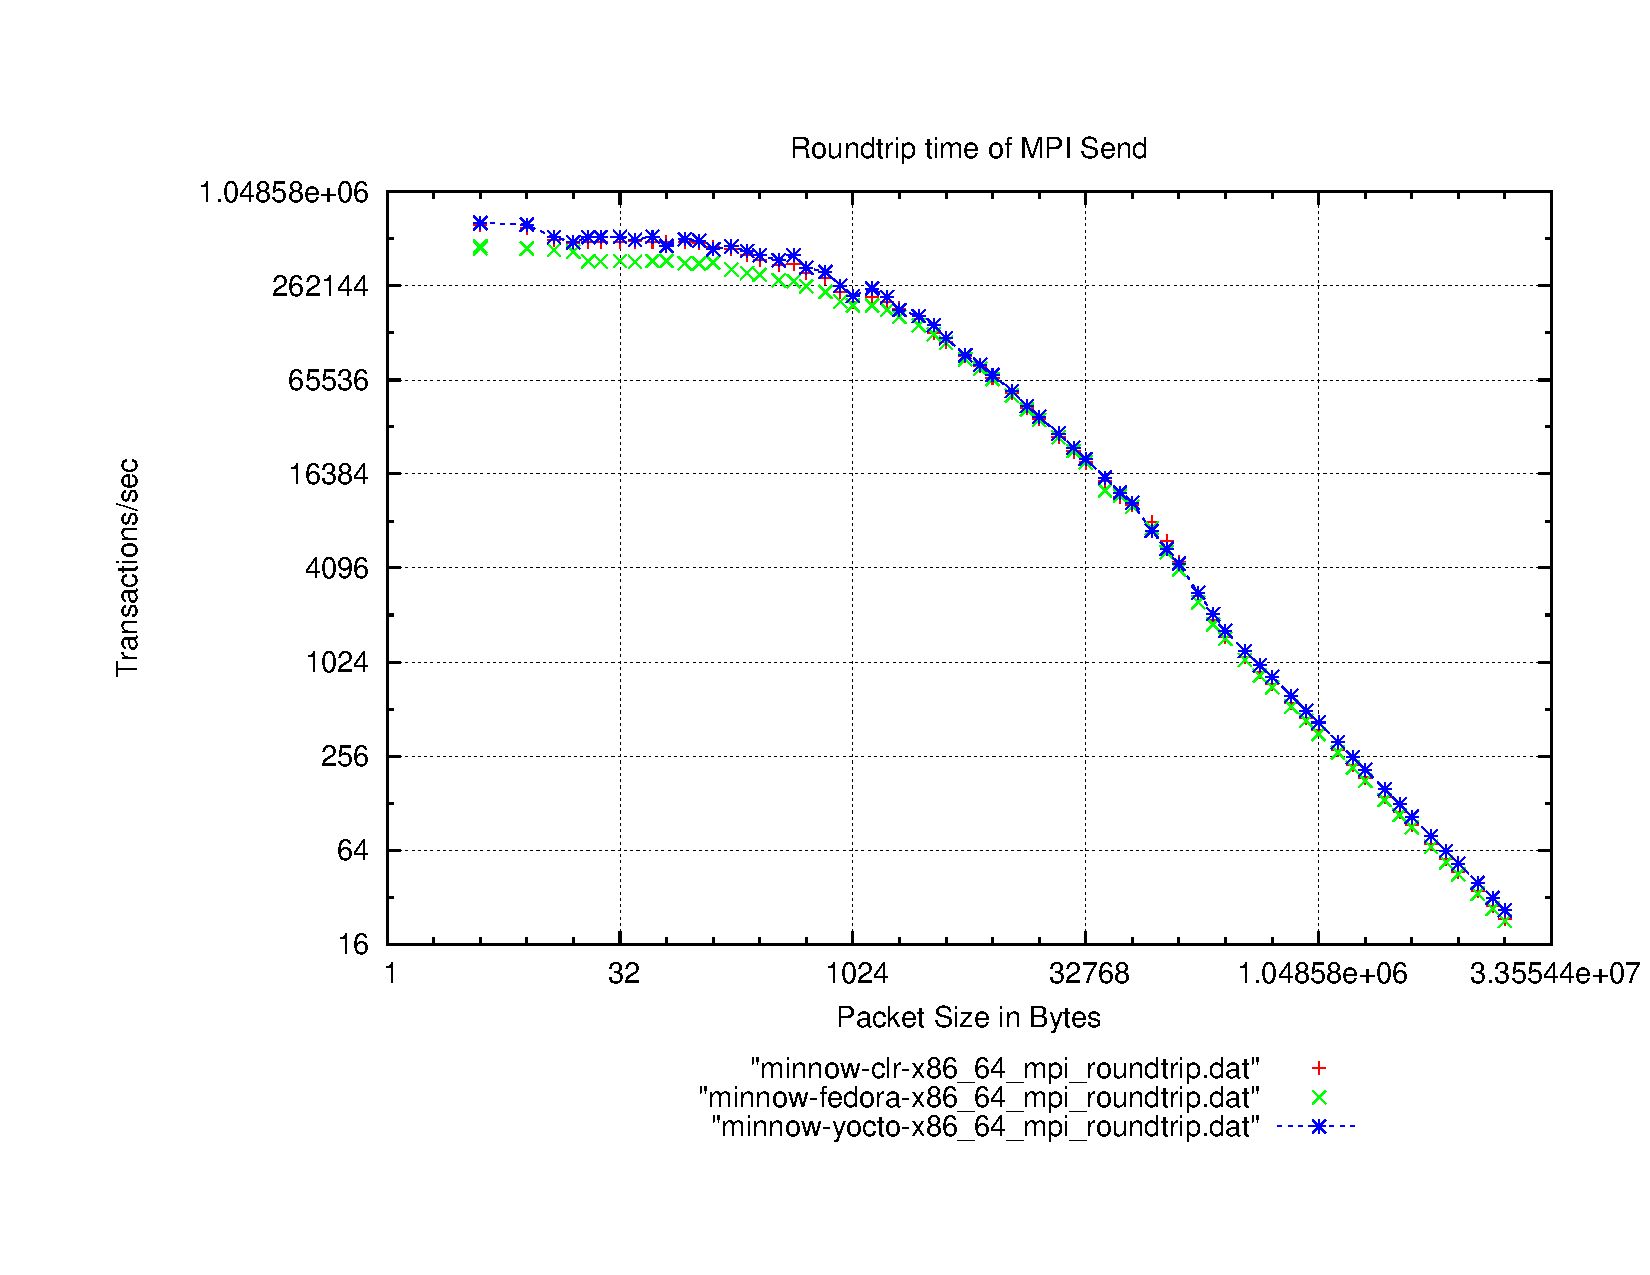
\includegraphics[width=0.75\textwidth]{images/mpbench_yocto_experiments/mpi_roundtrip.pdf}
\caption{MPI Bi directional bandwidth running in Minnowboard with Clear Linux,
Yocto and Fedora (lower is better)}
\label{mpi_roundtrip_yocto}
\end{figure}

Latency and bandwidth tests ( figure \ref{mpi_latency_yocto} and figure
\ref{mpi_roundtrip_yocto}) have the same performance despite the Operating
System running on the platform under test ( Minnow Board Max , due to the fact
that we are running the tests in a single platform for now.


\section{Compare MPI benchmark performance of cluster of embedded systems
against traditional computing system}

    \begin{center}
    \begin{tabular}{ | l | r |}
        \hline
        Platform under test & Minnow Board  Max and Intel NUC D54250WYK
        (Haswell)\\ \hline
        Number of platforms  & 6  \\ \hline
        Operating System & Yocto / Clear Linux  \\ \hline
        SW to Test & MPI benchmark \\ \hline
    \end{tabular}
    \end{center}

After doing the experiments in a single Atome system we decided to do the
experiments in a cluster of them. The experiment is limited to the number of
systems we can gather. In this case we could gather 6 Minnowboad
\cite{minnowboard} platforms to do the experiments. The full diagram of the
cluster is described bellow in figure \ref{fig:5.20}.

\begin{figure}[H]
\centering
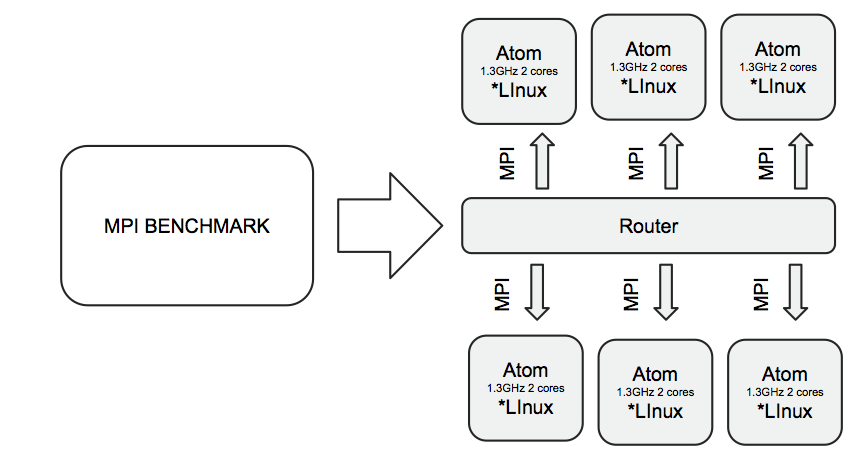
\includegraphics[width=0.75\textwidth]{images/cluster_minnows.png}
\caption{Connection Ports of the Minnow board Max}
\label{fig:5.20}
\end{figure}

All these systems execute the MPIBenchmarks with the following ssh config file:


\begin{lstlisting}[frame=single,language=bash]
  $ cat ~/.ssh/config
    Host node1
        HostName node1-ip-or-hostname
        User user-of-the-ssh-key
        Port port-if-nedded

    Host node2
        HostName node1-ip-or-hostname
        User user-of-the-ssh-key
        Port port-if-nedded

    Host node3
        HostName node1-ip-or-hostname
        User user-of-the-ssh-key
        Port port-if-nedded

\end{lstlisting}

And the following MPI config file:


\begin{lstlisting}[frame=single,language=bash]
  $ cat hostfile
    node1
    node2
    node3
\end{lstlisting}

This is necessary to make the systems communicate each other through MPI , if we
don't include this configuration there will not be any communications due to the
fact that MPI requires an ssh connection. 

The idea of this experiment is to compare the performance of the cluster of
Embedded systems (now that we have found that a Yocto base OS has the best
performance) with a Traditional Computing System. In this case it will be the
Intel NUC D54250WYK (Haswell). The brief description of this system is
described here in following table: 

    \begin{center}
    \begin{tabular}{ | l | r |}
        \hline
        Platform Name & Intel NUC D54250WYK \\ \hline
        Core Name & i5-4250U CPU  \\ \hline
        Number of cores & 2 \\ \hline
        Number of Threads & 4 \\ \hline
        Frequency & 1.30GHz \\ \hline
        Memory & 16GB\\ \hline
        Hard Disk & 120GB \\ \hline
    \end{tabular}
    \end{center}



\subsection{Results}

After executing the MPI benchmark in the cluster of embedded systems  and in
the NUC ( with Clear Linux OS ) we could compare their MPI performance in the
following graphs; 


\begin{figure}[H]
\centering
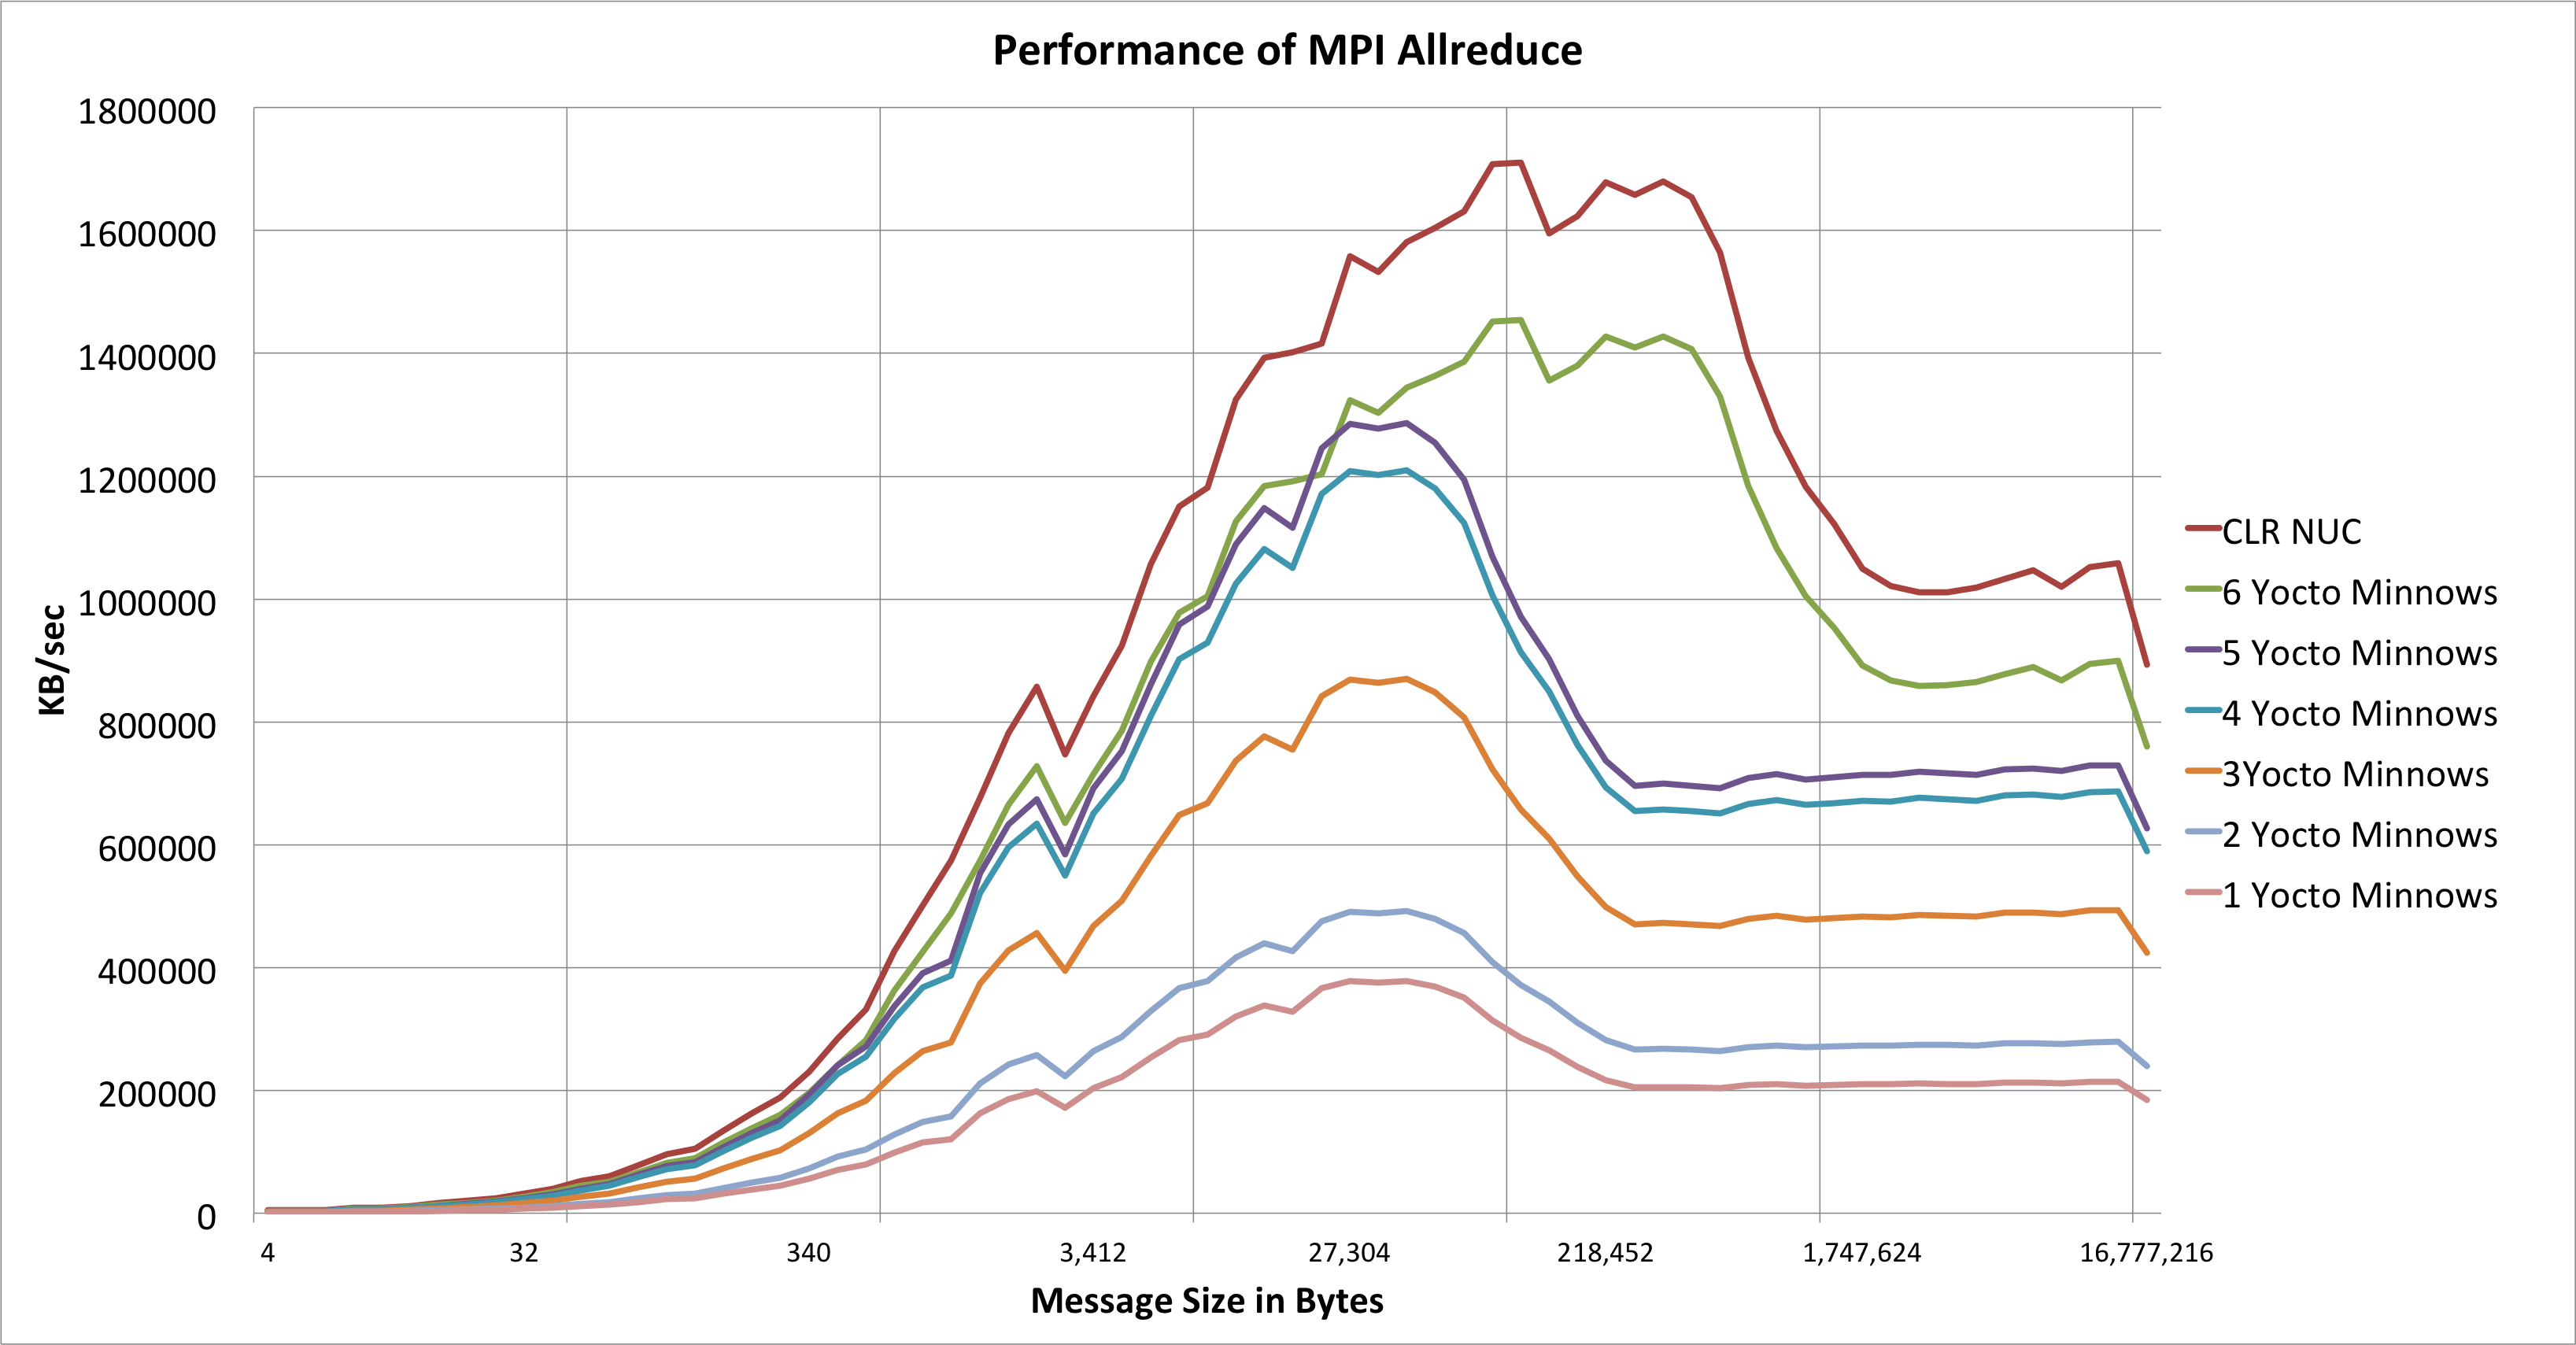
\includegraphics[width=1.0\textwidth]{images/mpbench_cluster_experiments/mpi_all_reduce.png}
\caption{All reduce  benchmark in cluster of minnowboards with Yocto OS and NUC
with Clear Linux OS}
\label{all_reduce_cluster}
\end{figure}


\begin{figure}[H]
\centering
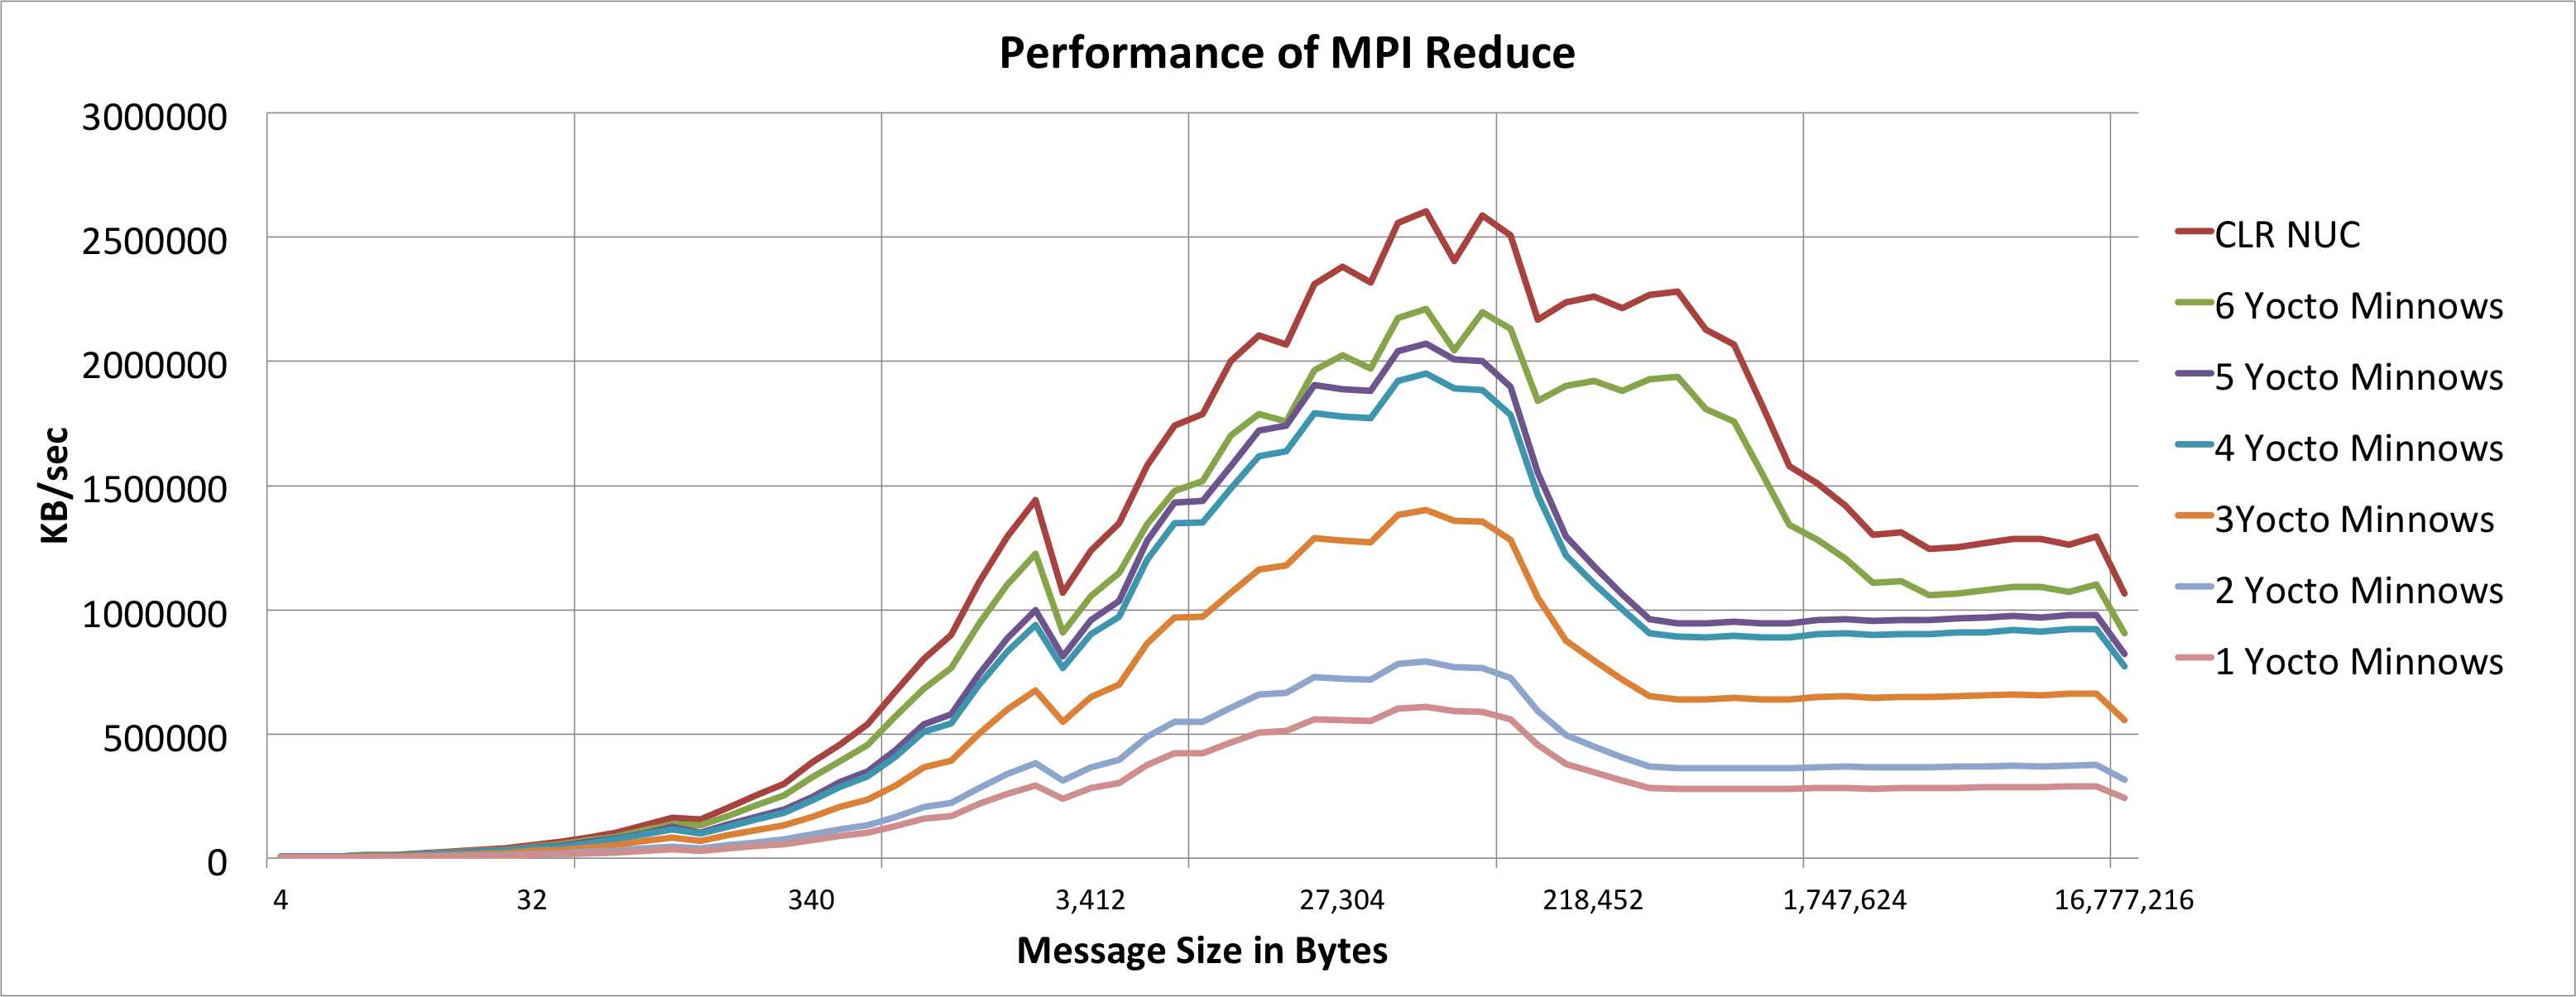
\includegraphics[width=1.0\textwidth]{images/mpbench_cluster_experiments/mpi_reduce.png}
\caption{Reduce  benchmark in cluster of minnowboards with Yocto OS and NUC
with Clear Linux OS}
\label{reduce_cluster}
\end{figure}



\begin{figure}[H]
\centering
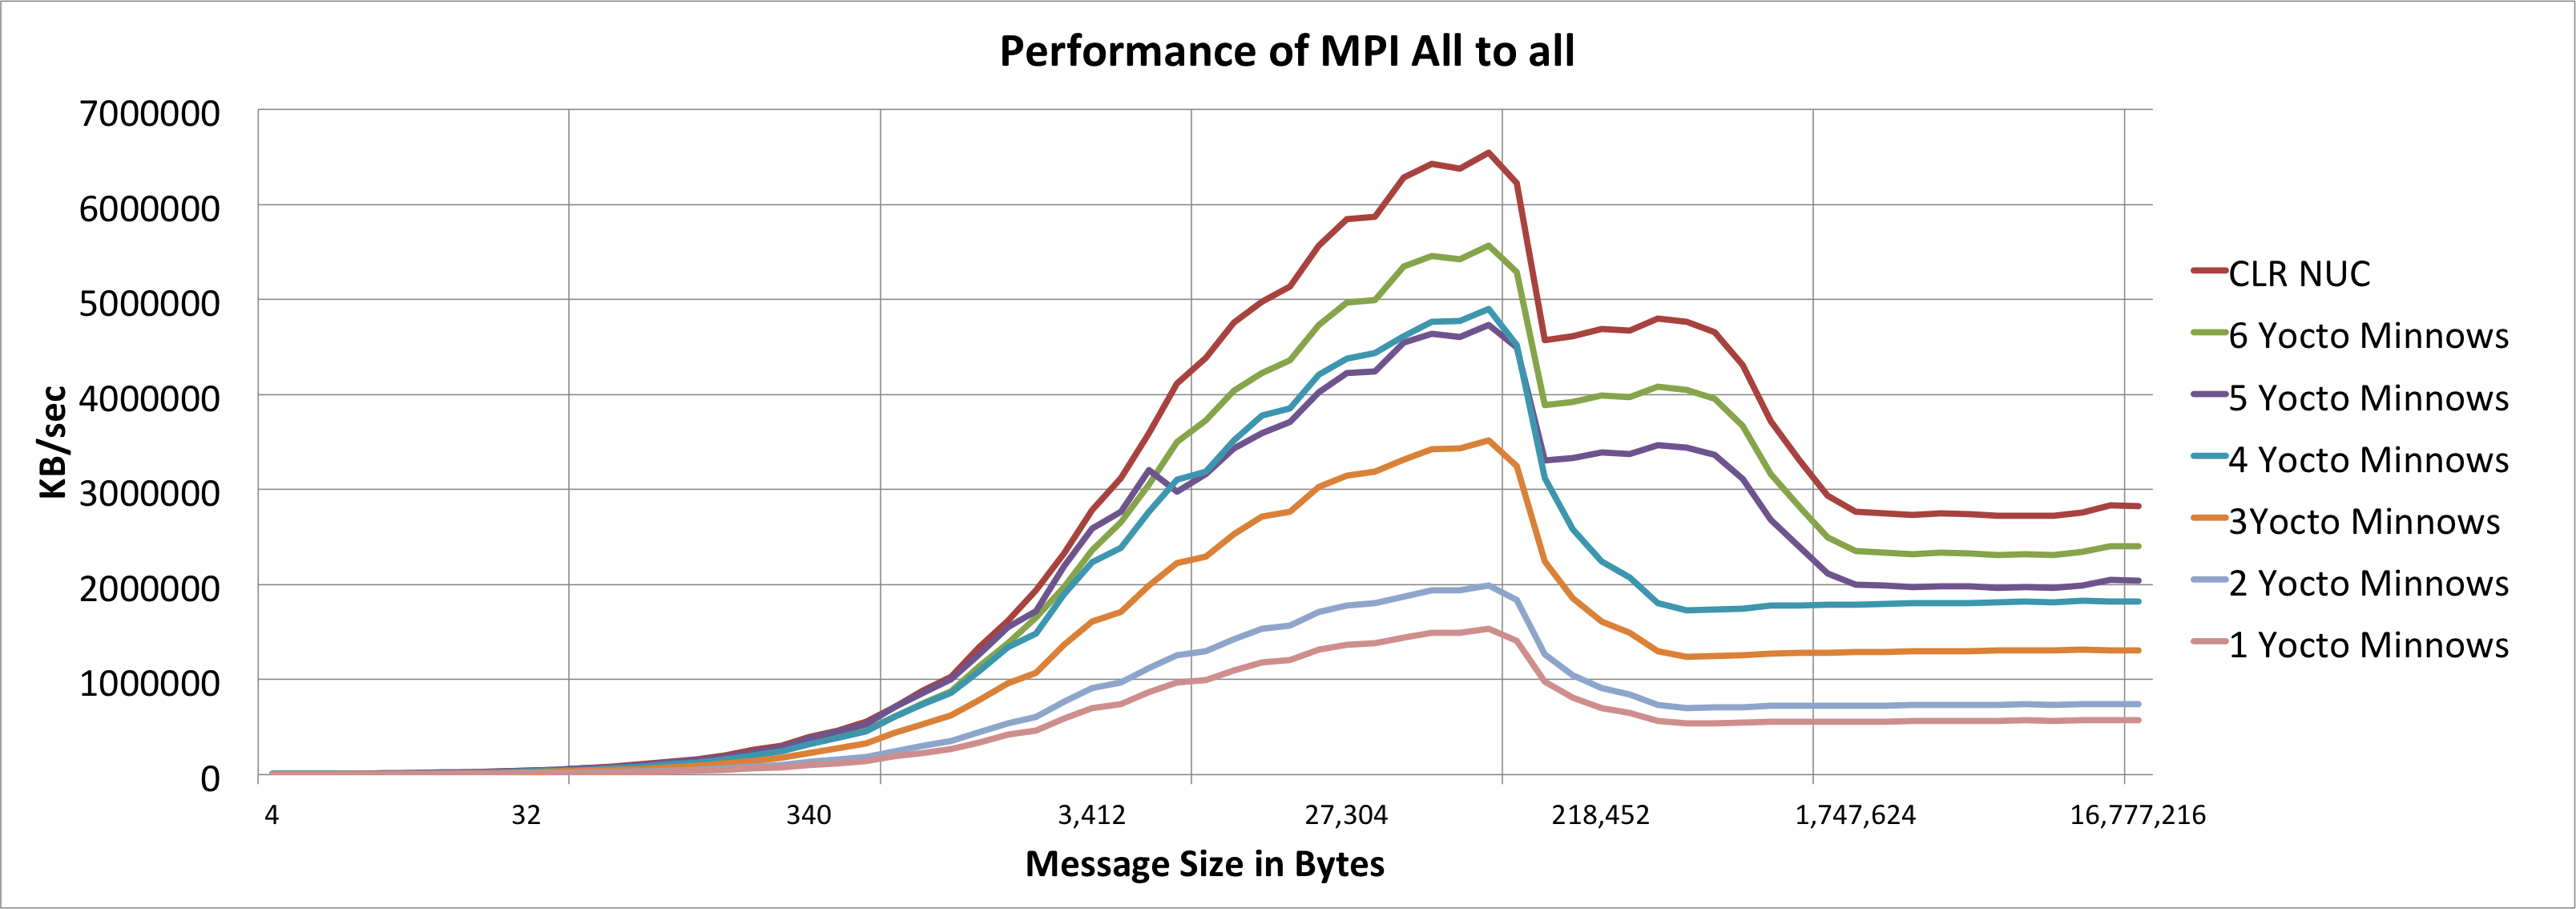
\includegraphics[width=1.0\textwidth]{images/mpbench_cluster_experiments/mpi_alltoall.png}
\caption{All to All  benchmark in cluster of minnowboards with Yocto OS and NUC
with Clear Linux OS}
\label{all_to_all_cluster}
\end{figure}


\begin{figure}[H]
\centering
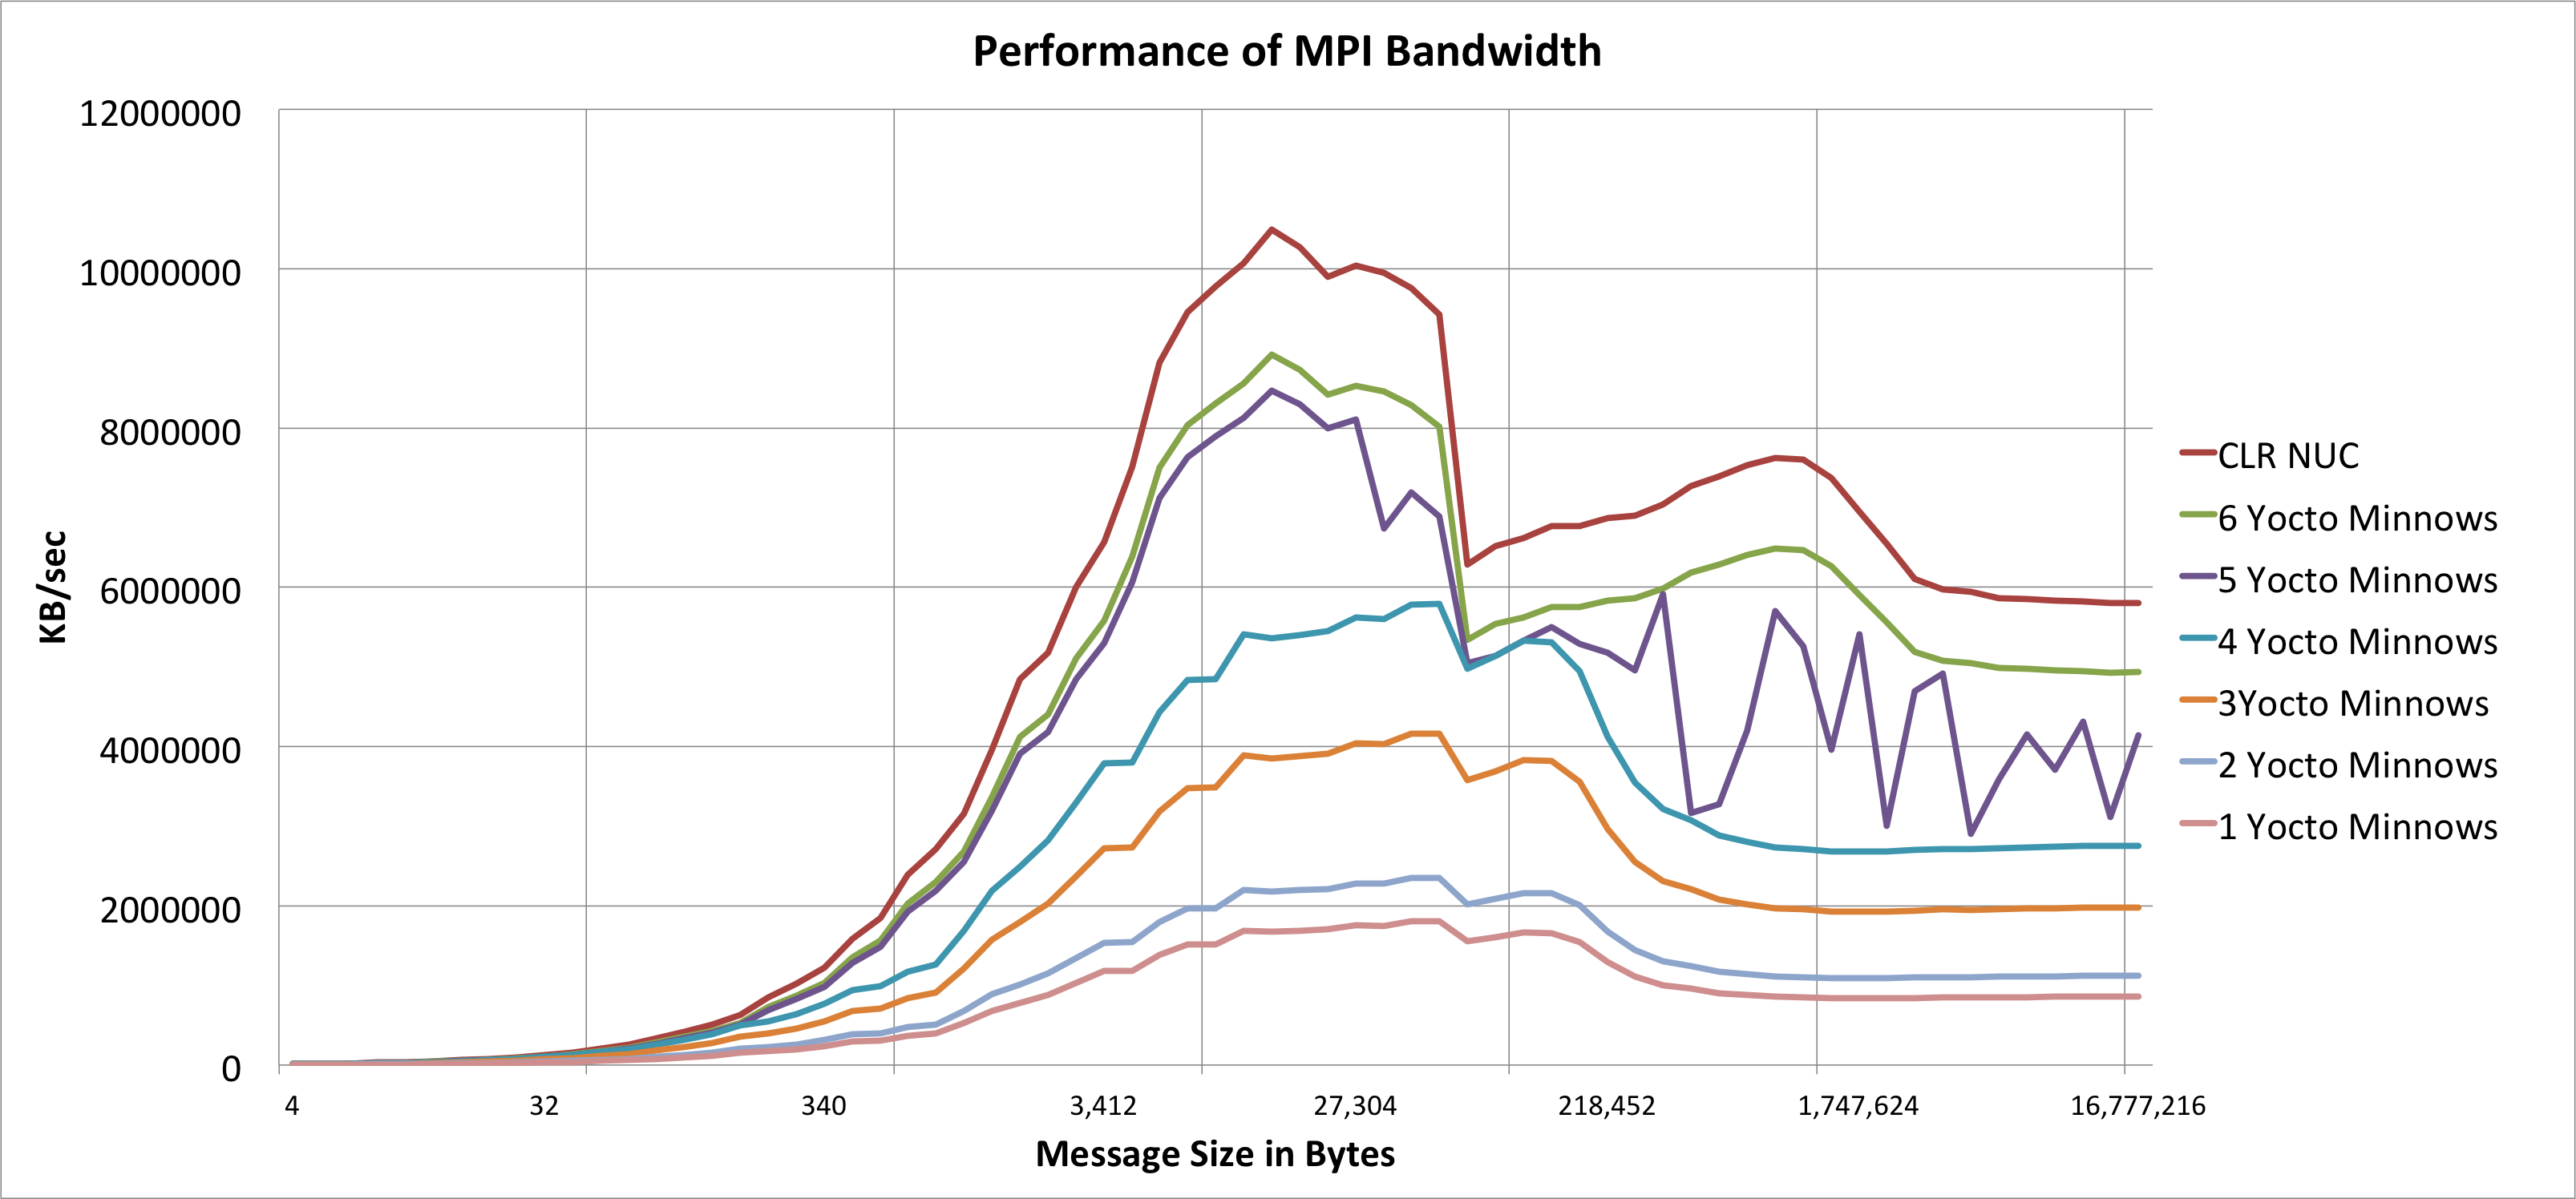
\includegraphics[width=1.0\textwidth]{images/mpbench_cluster_experiments/mpi_bandwidth.png}
\caption{Bandwidth  benchmark in cluster of minnowboards with Yocto OS and NUC
with Clear Linux OS}
\label{all_to_all_cluster}
\end{figure}

\begin{figure}[H]
\centering
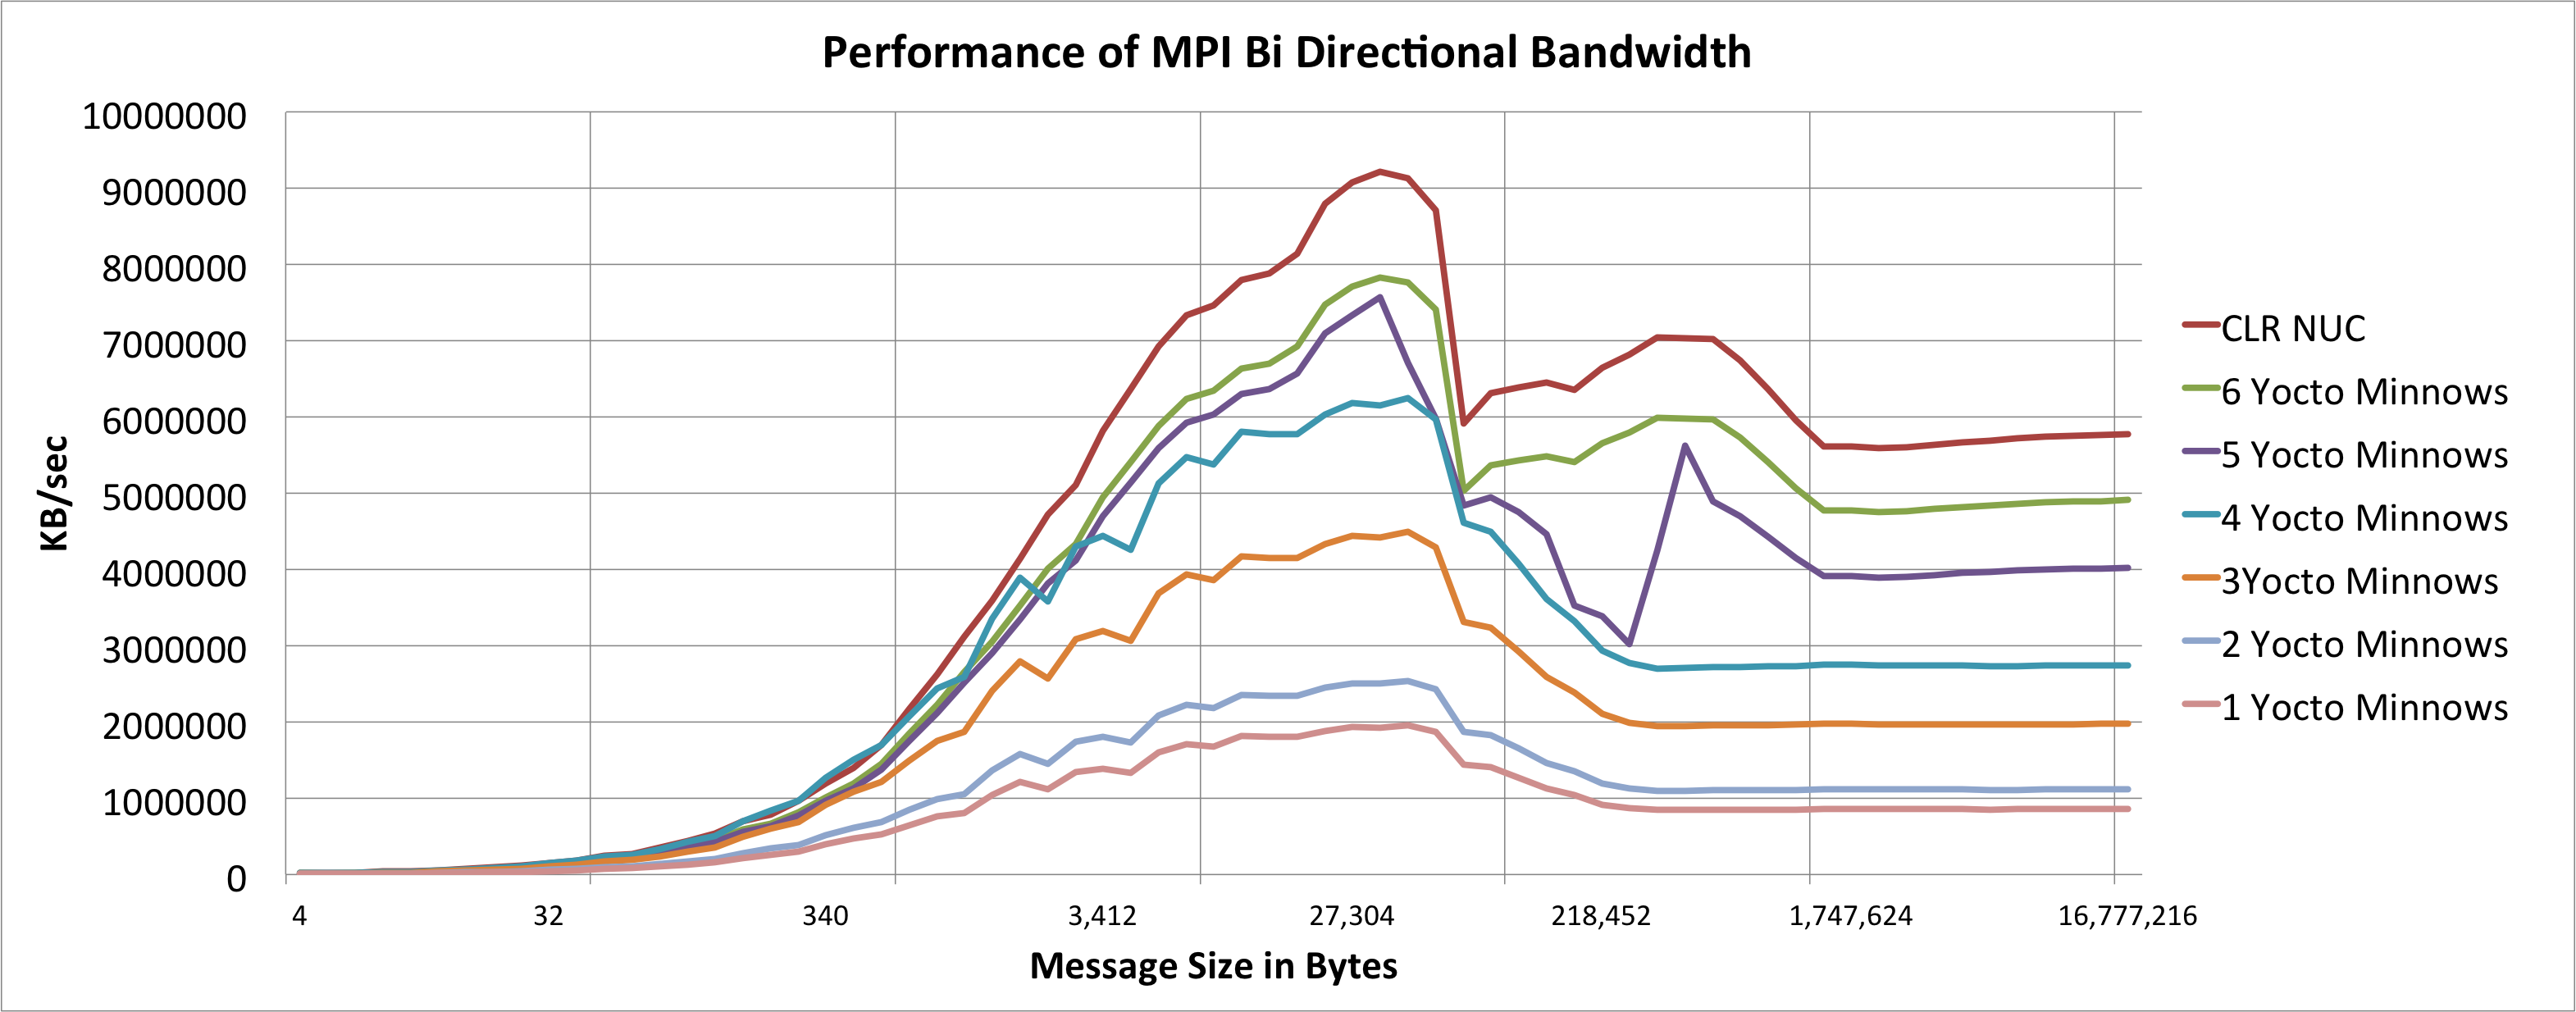
\includegraphics[width=1.0\textwidth]{images/mpbench_cluster_experiments/mpi_bibw.png}
\caption{Bi directional bandwidth benchmark in cluster of minnowboards with Yocto OS and NUC
with Clear Linux OS}
\label{all_to_all_cluster}
\end{figure}


\begin{figure}[H]
\centering
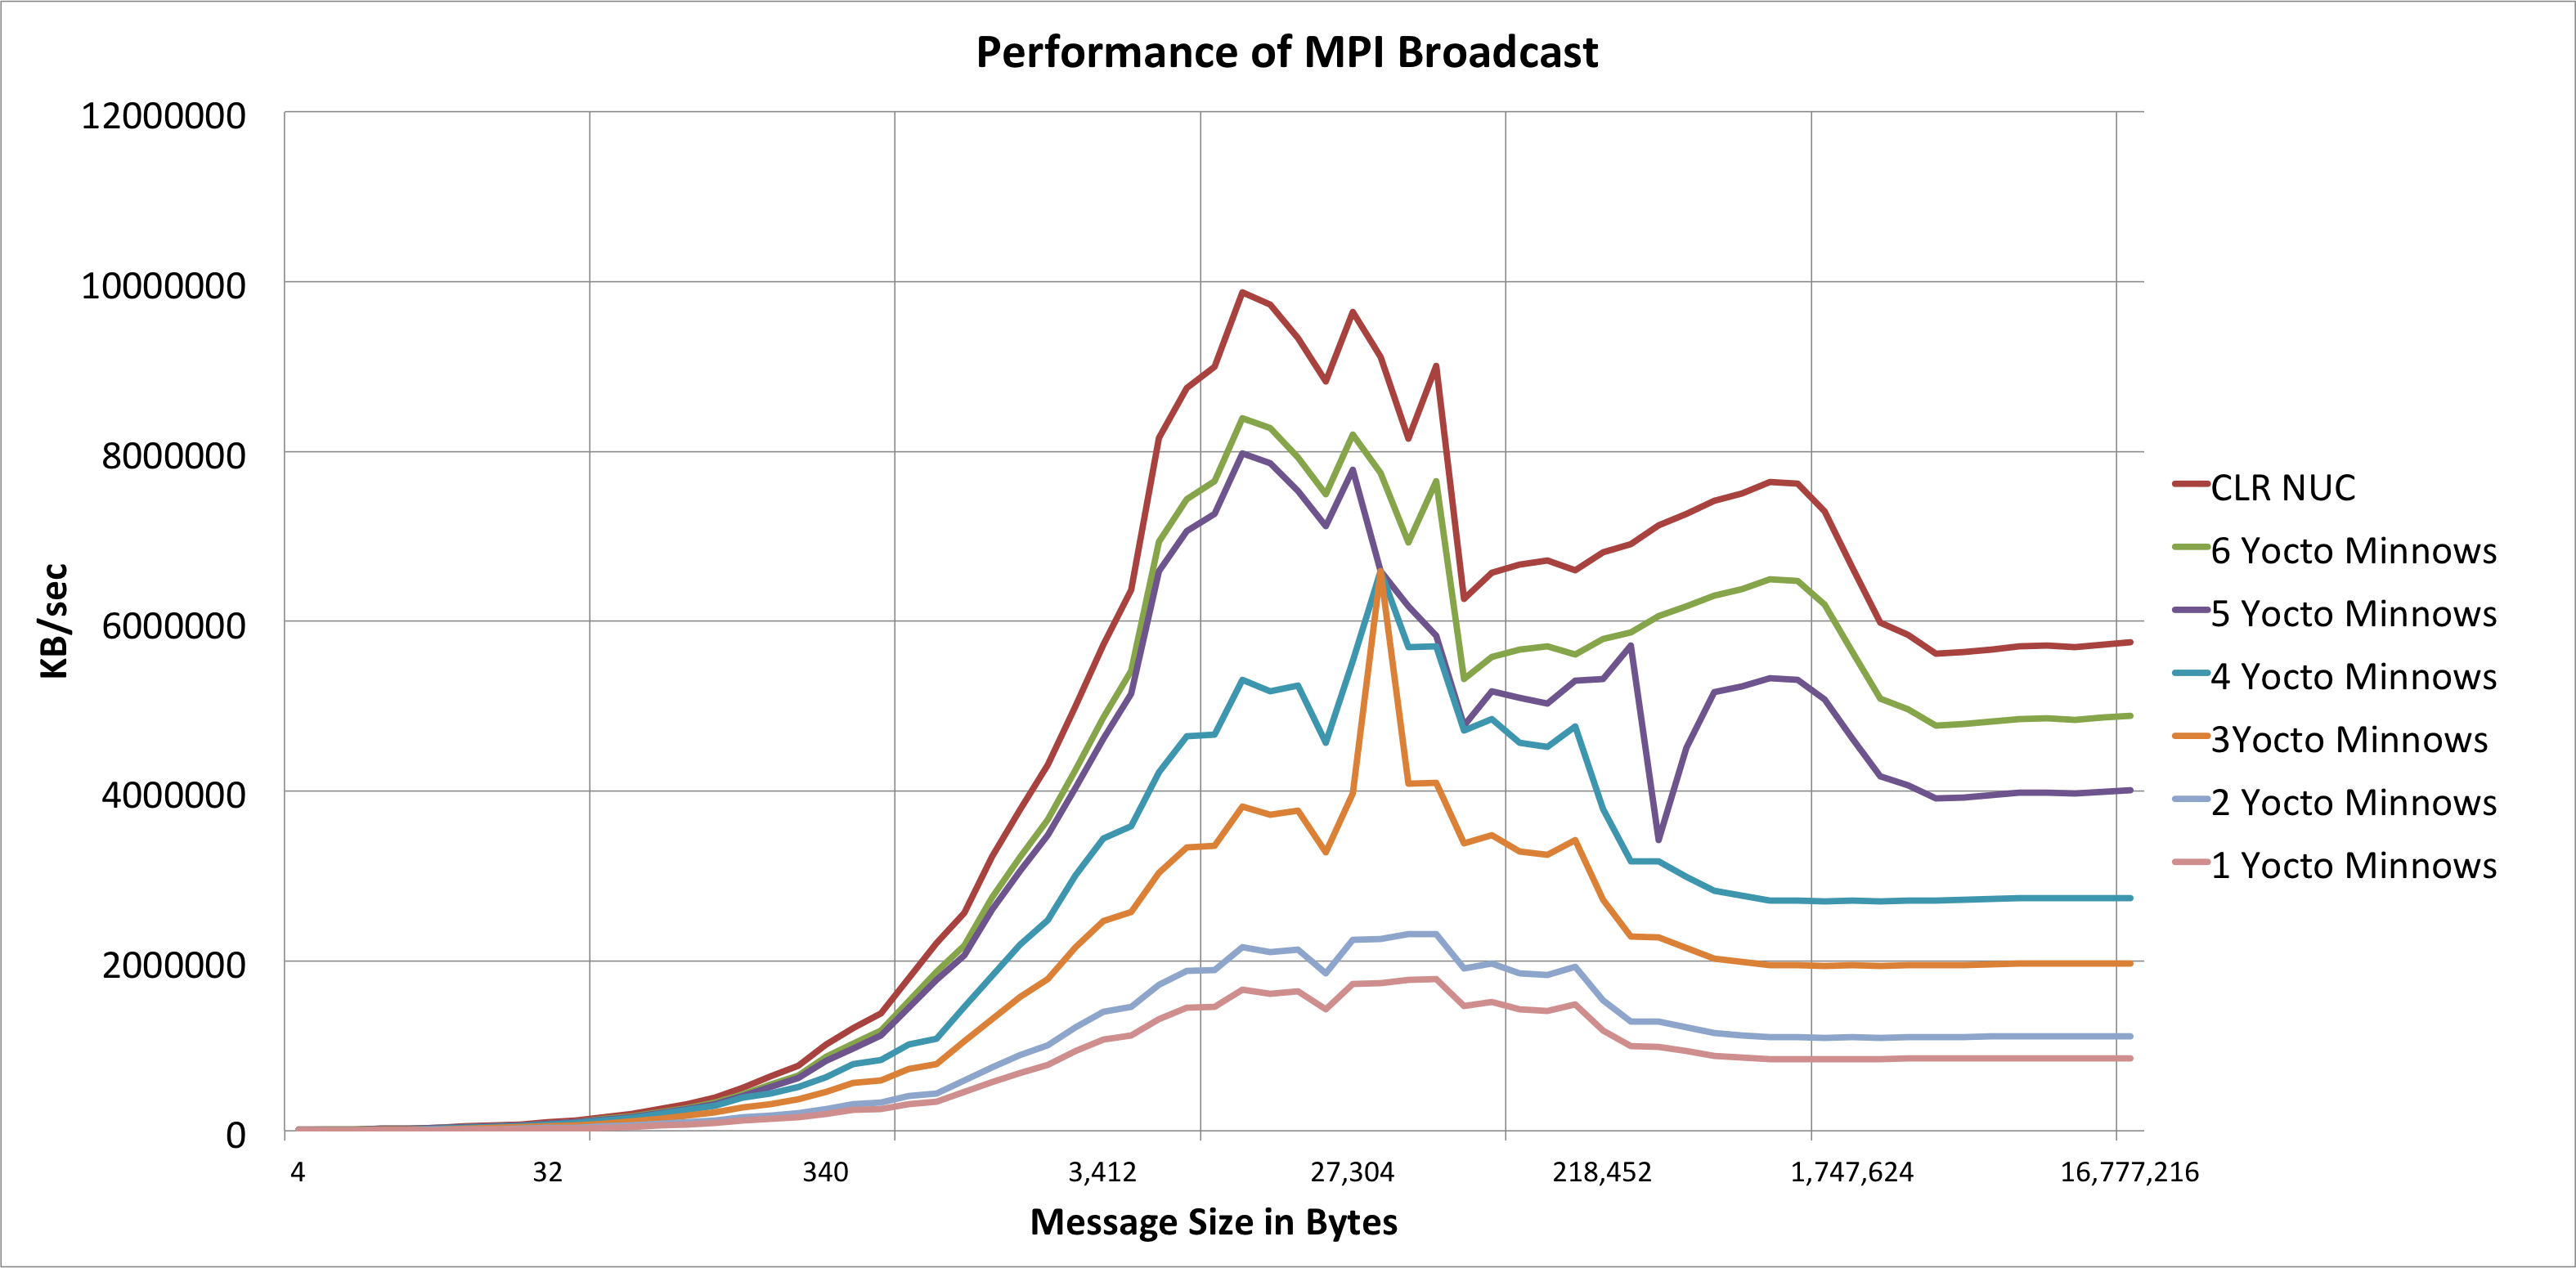
\includegraphics[width=1.0\textwidth]{images/mpbench_cluster_experiments/mpi_broadcast.png}
\caption{Broadcast  benchmark in cluster of minnowboards with Yocto OS and NUC
with Clear Linux OS}
\label{all_to_all_cluster}
\end{figure}

\begin{figure}[H]
\centering
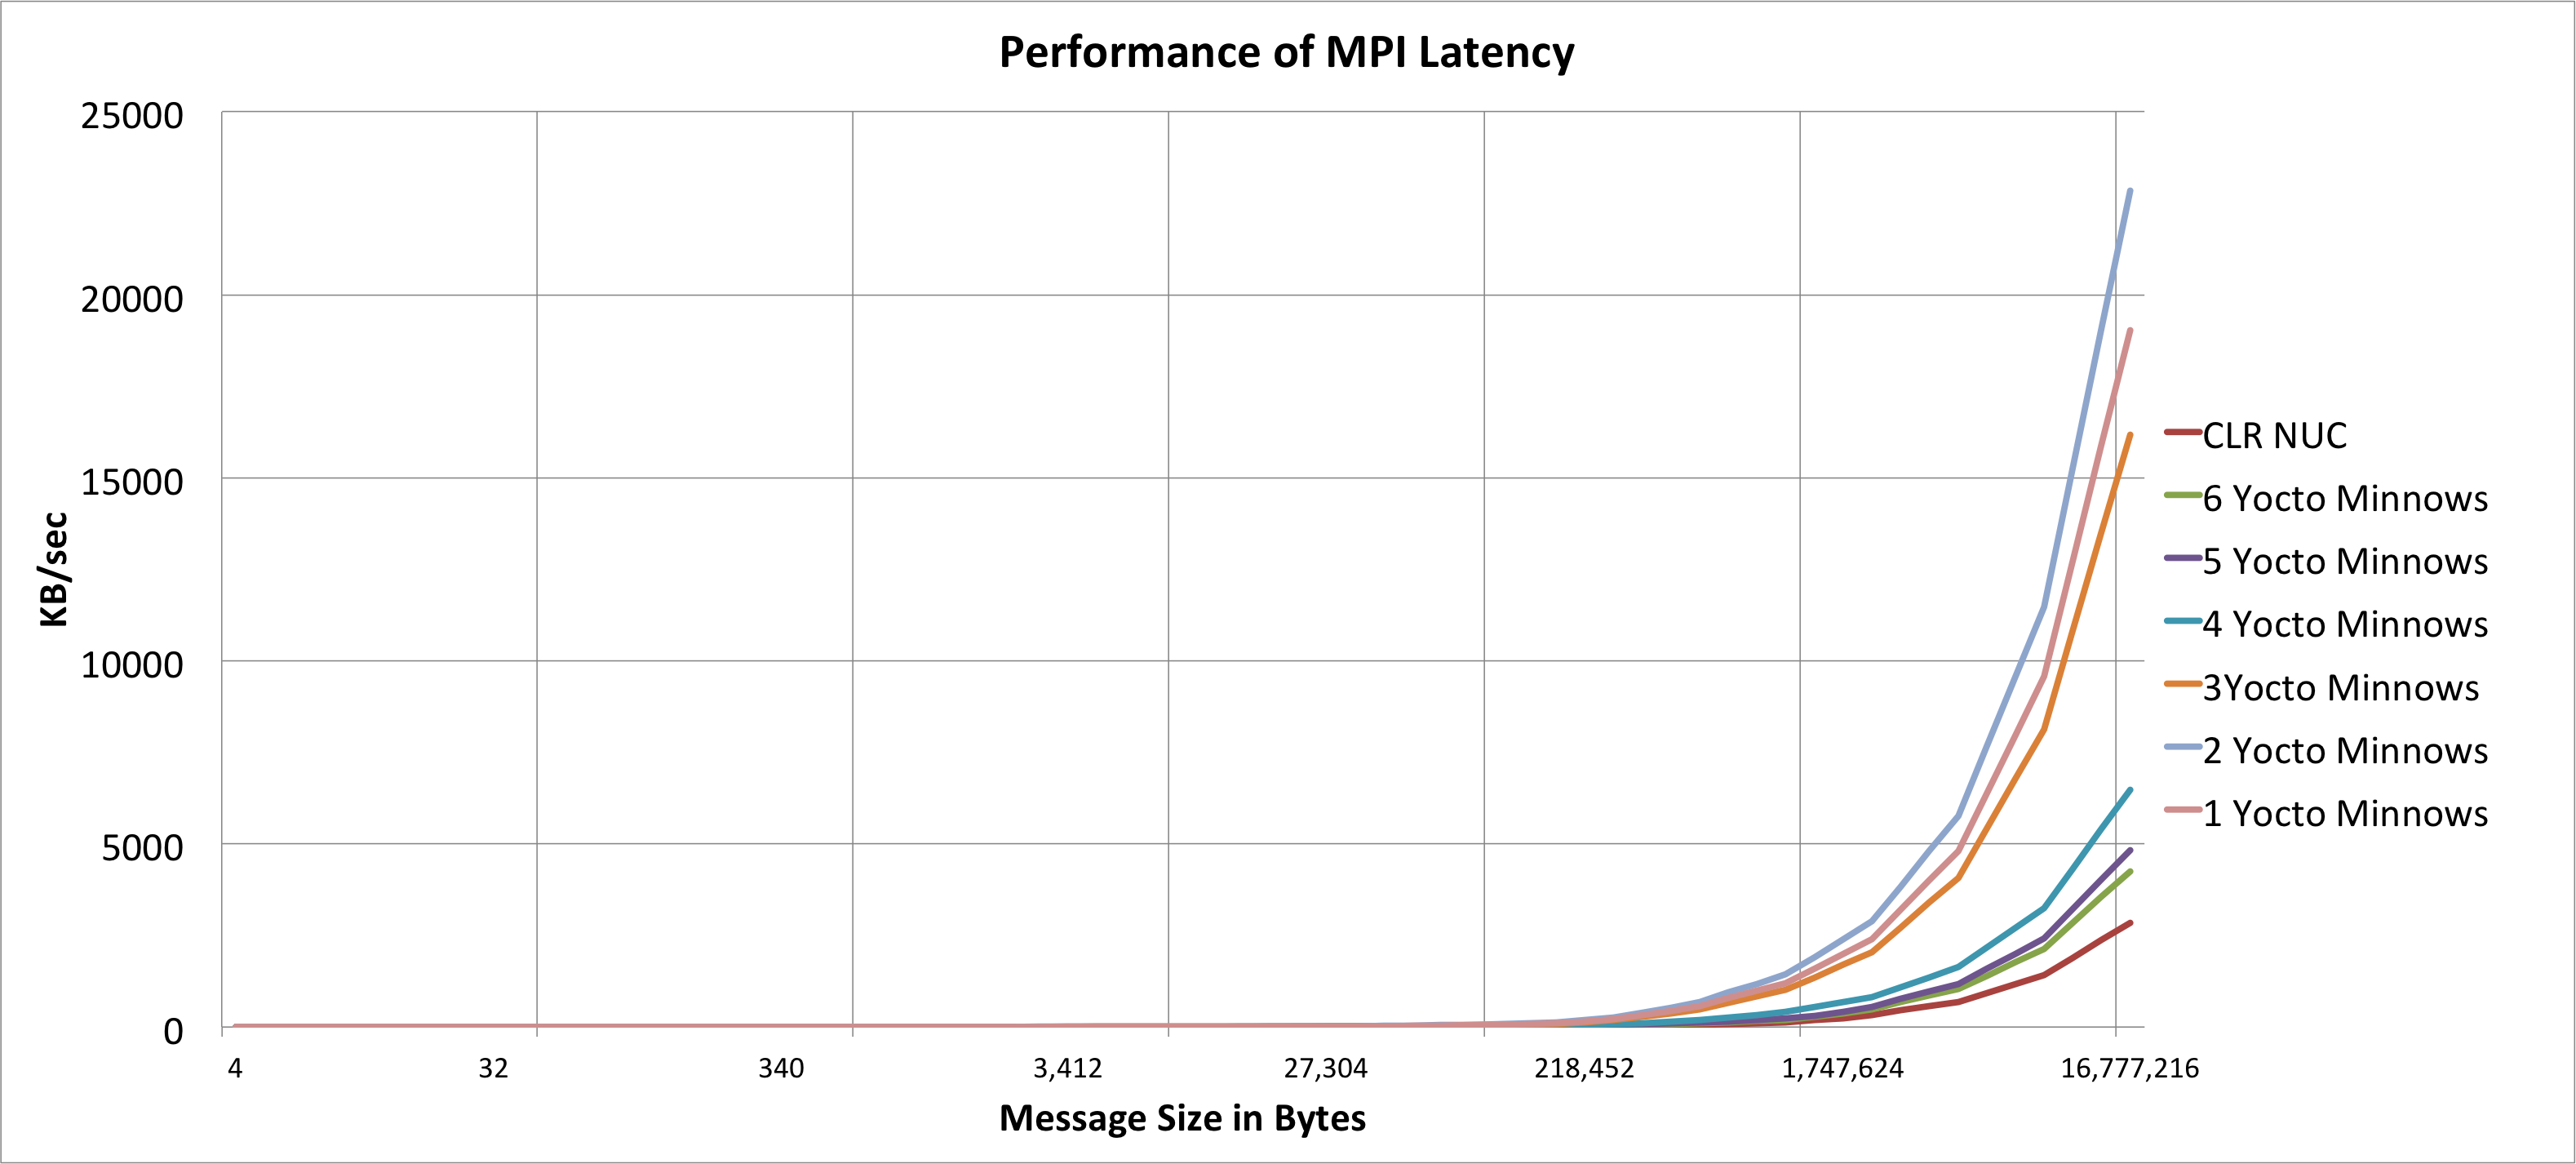
\includegraphics[width=1.0\textwidth]{images/mpbench_cluster_experiments/mpi_latency.png}
\caption{Latency  benchmark in cluster of minnowboards with Yocto OS and NUC
with Clear Linux OS}
\label{all_to_all_cluster}
\end{figure}


\begin{figure}[H]
\centering
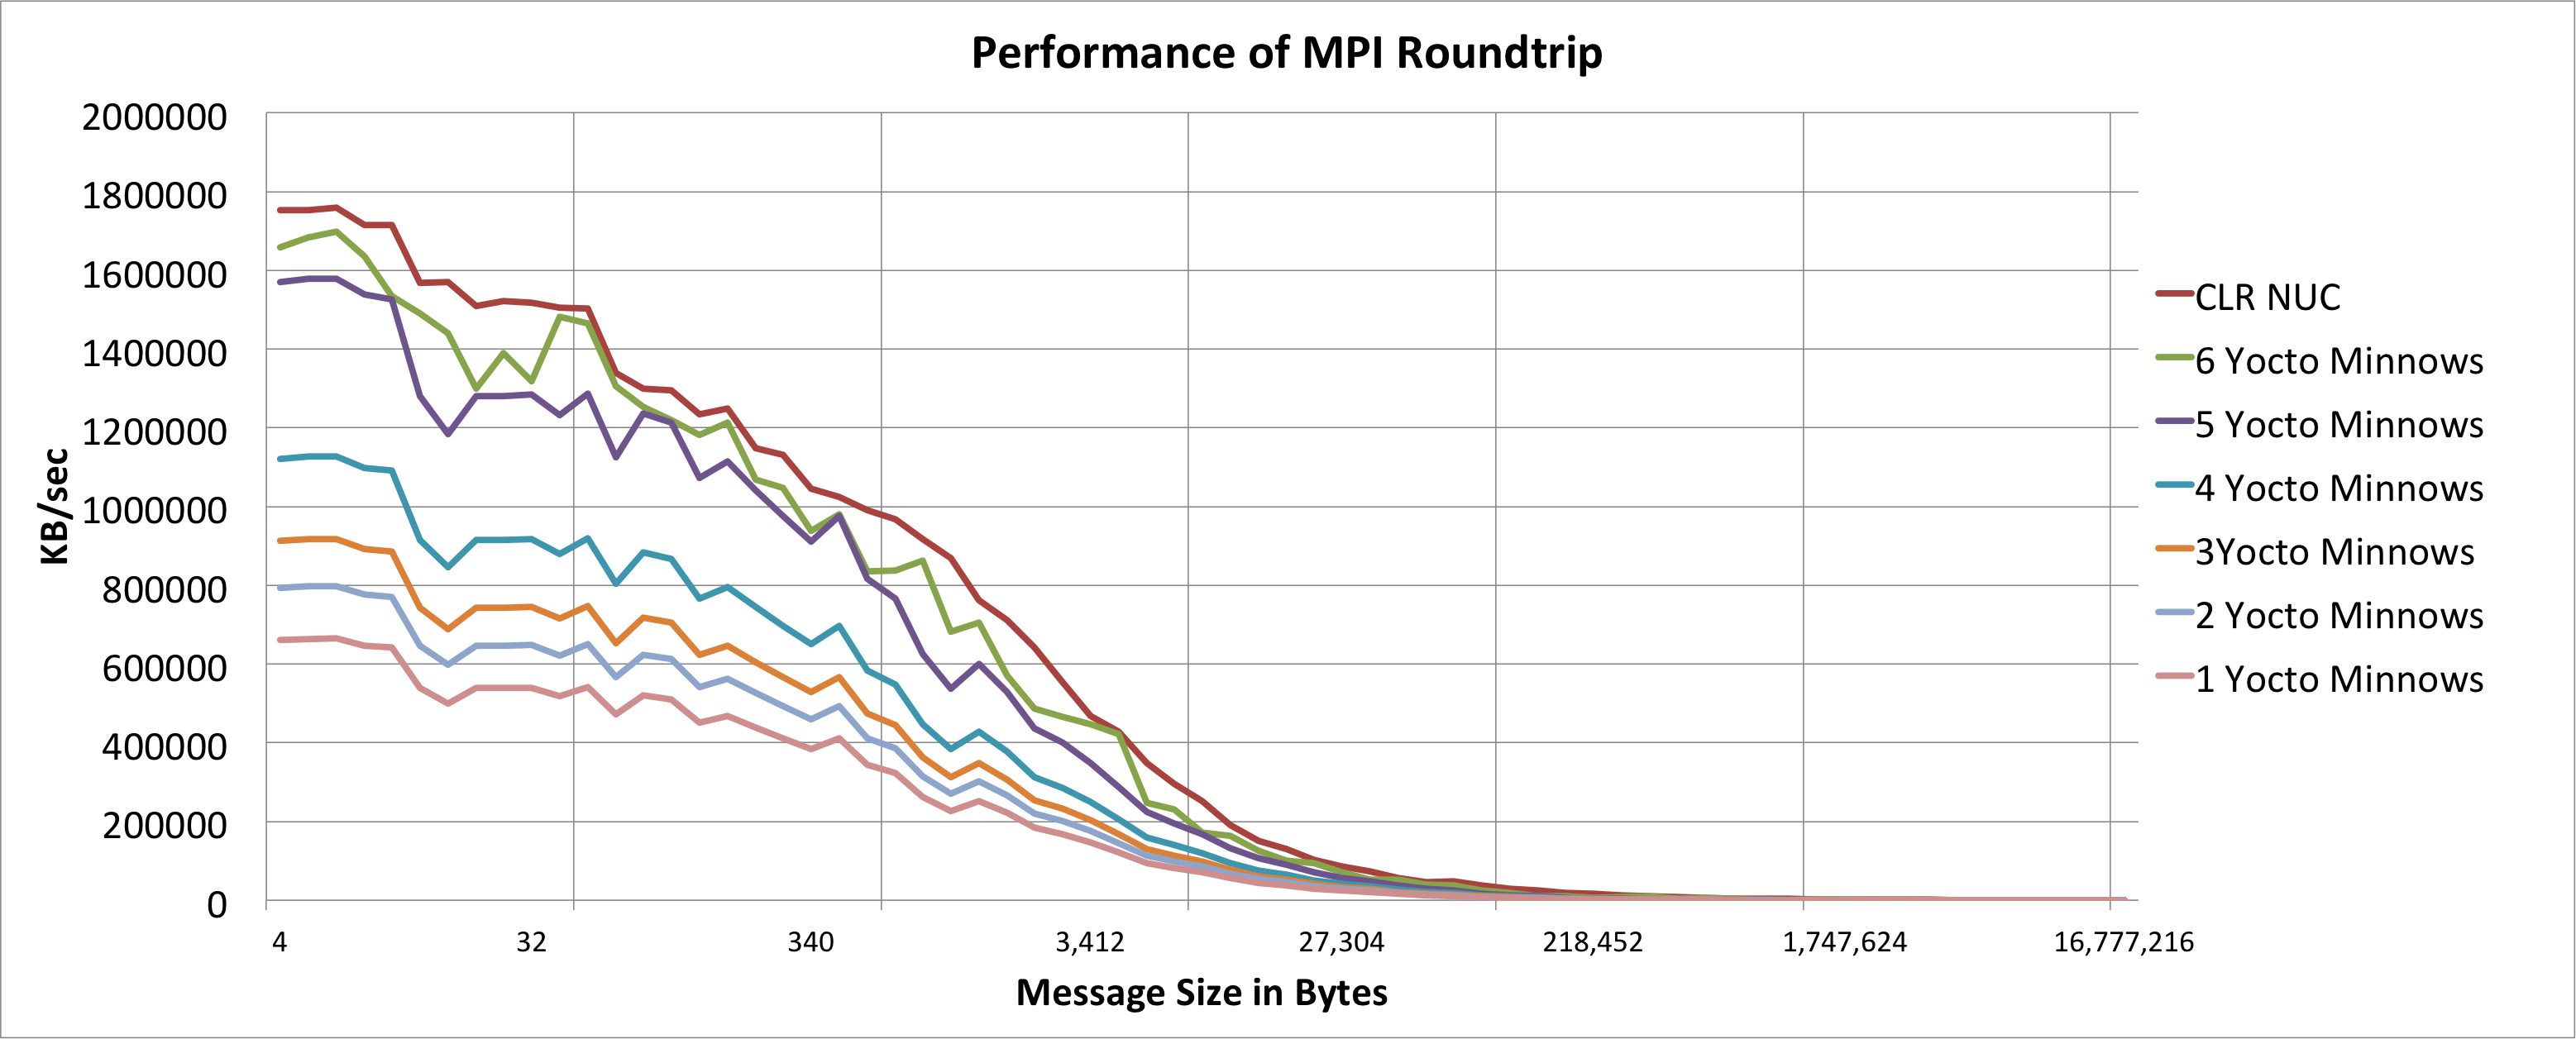
\includegraphics[width=1.0\textwidth]{images/mpbench_cluster_experiments/mpi_roundtrip.png}
\caption{Roundtrip  benchmark in cluster of minnowboards with Yocto OS and NUC
with Clear Linux OS}
\label{all_to_all_cluster}
\end{figure}



\section{Compare power efficiency of cluster of embedded systems against
traditional computing system}


So far we have been able to see the performance comparison of a traditional
computer system and a cluster of embedded systems. As we have seen even with 6
systems of embedded platforms is not possible to get the same performance
impact that with traditional computer system ( close , upt 85\% of the
performance in some tests ) ; but what about the power consumption?. If we
remember the hypothesis (Section 1.4) The part that we are concern is to
determine the breaking point where is better to send the data to the cloud data
centers. How many systems is the maximum that these kind of network could
support and still being a good option in terms of energy efficiency?

In computing, performance per watt is a measure of the energy efficiency of a
particular computer architecture or computer hardware. Literally, it measures
the rate of computation that can be delivered by a computer for every watt of
power consumed.

\begin{equation}
    Energy Efficiency = \dfrac {Performance}{Watts}
\end{equation}

We believe that the energy efficiency in an embedded cluster will have the
behavior of the  figure~\ref{fig:1.2}. In the beginning the increment of the
number of nodes in our network will increment the performance (the top part of
the equation), but at the same time the amount of watts will
increase making the energy efficiency flat at some point (if the lower part of
the equation increases the equation tends to decrease)

The next natural step is to measure the power consumption of both systems : the
cluster of embedded systems and the D54250WYK

The instrument to measure the power consumption of the system is the WT300
Series Digital Power Meter (from Yokogawa) . Digital Power Analyzers are
instruments for laboratory, manufacturing test, or handheld applications to
accurately measure and analyze electrical power characteristics.

The next table \ref{minnow_power_1} describe the power consumption of a single Minnow board: 

\begin{table}[]
    \centering
    \resizebox{\textwidth}{!}{
    \begin{tabular}{|l|l|l|l|l|l|l|l|l|}
    \hline
          &All reduce &Reduce & All to all &Bandwidht & Bi direct bandwidth & Boradcast & Latency & Roundtrip \\ \hline 
          Average Power Consumption (Watts) & 4.234  & 2.231 & 2.4.876 & 4.9871 & 4.7865 & 4.8721  & 4.1235  & 4.8563 \\ \hline
          MAX Watts & 5.6139 & 5.875 & 5.934 & 5.823 & 5.749  & 5.853 & 5.761 & 5.703 \\ \hline
          MIN Watts & 2.8874 & 2.234 & 2.7532 & 2.8342 & 2.7431  & 2.6548 & 2.934  & 2.985 \\ \hline
          Average Power at idle (Watts) & 2.5663 & 2.5663 & 2.5663 & 2.5663 & 2.5663 & 2.5663 & 2.5663  & 2.5663 \\ \hline
    \end{tabular}}
    \captionof{table}{Minnow board Max power consumption during MPI bench}
    \label{minnow_power_1}
\end{table}


The next table describe the power consumption of a single NUC D54250WYK


\begin{table}[]
    \centering
    \resizebox{\textwidth}{!}{
    \begin{tabular}{|l|l|l|l|l|l|l|l|l|}
    \hline
          & All reduce & Reduce  & All to all &
          Bandwidht & Bi directional bandwidth &
          Boradcast & Latency & Roundtrip \\ \hline
          Average Power Consumption (Watts) &
          18.0742    & 19.2853 & 18.6589    &
          18.2385   & 18.8423                  &
          19.4739   & 18.8664 & 19.6473   \\ \hline
          MAX Watts                         &
          20.3010    & 20.1011 & 20.4240    &
          20.8761   & 19.9573                  &
          20.8436   & 20.3242 & 20.3452   \\ \hline
          MIN Watts                         &
          5.2046     & 4.4239  & 5.9853     &
          6.5838    & 5.4086                   &
          4.5973    & 6.2199  & 6.8419    \\ \hline
          Average Power at idle (Watts)     &
          4.4801     & 4.4801  & 4.4801     &
          4.4801    & 4.4801                   &
          4.4801    & 4.4801  & 4.4801    \\ \hline
        \end{tabular}}
    \caption{NUC D54250WYK power consumption during MPI bench}
    \label{NUC_power_1}
\end{table}


As we can see the average power consumption of the NUC is close to 20 Watts in
the meantime the average power consumption of the embedded system is close to
2 Watts. This is due to the design of the embedded system, just the CPU in the
embedded system is designed to consume 1 Watt in idle mode.

After this we start to measure the power consumption of the embedded cluster,
this can bee seen in the next graph\ref{power_average_minnow}: 

\begin{figure}[H]
\centering
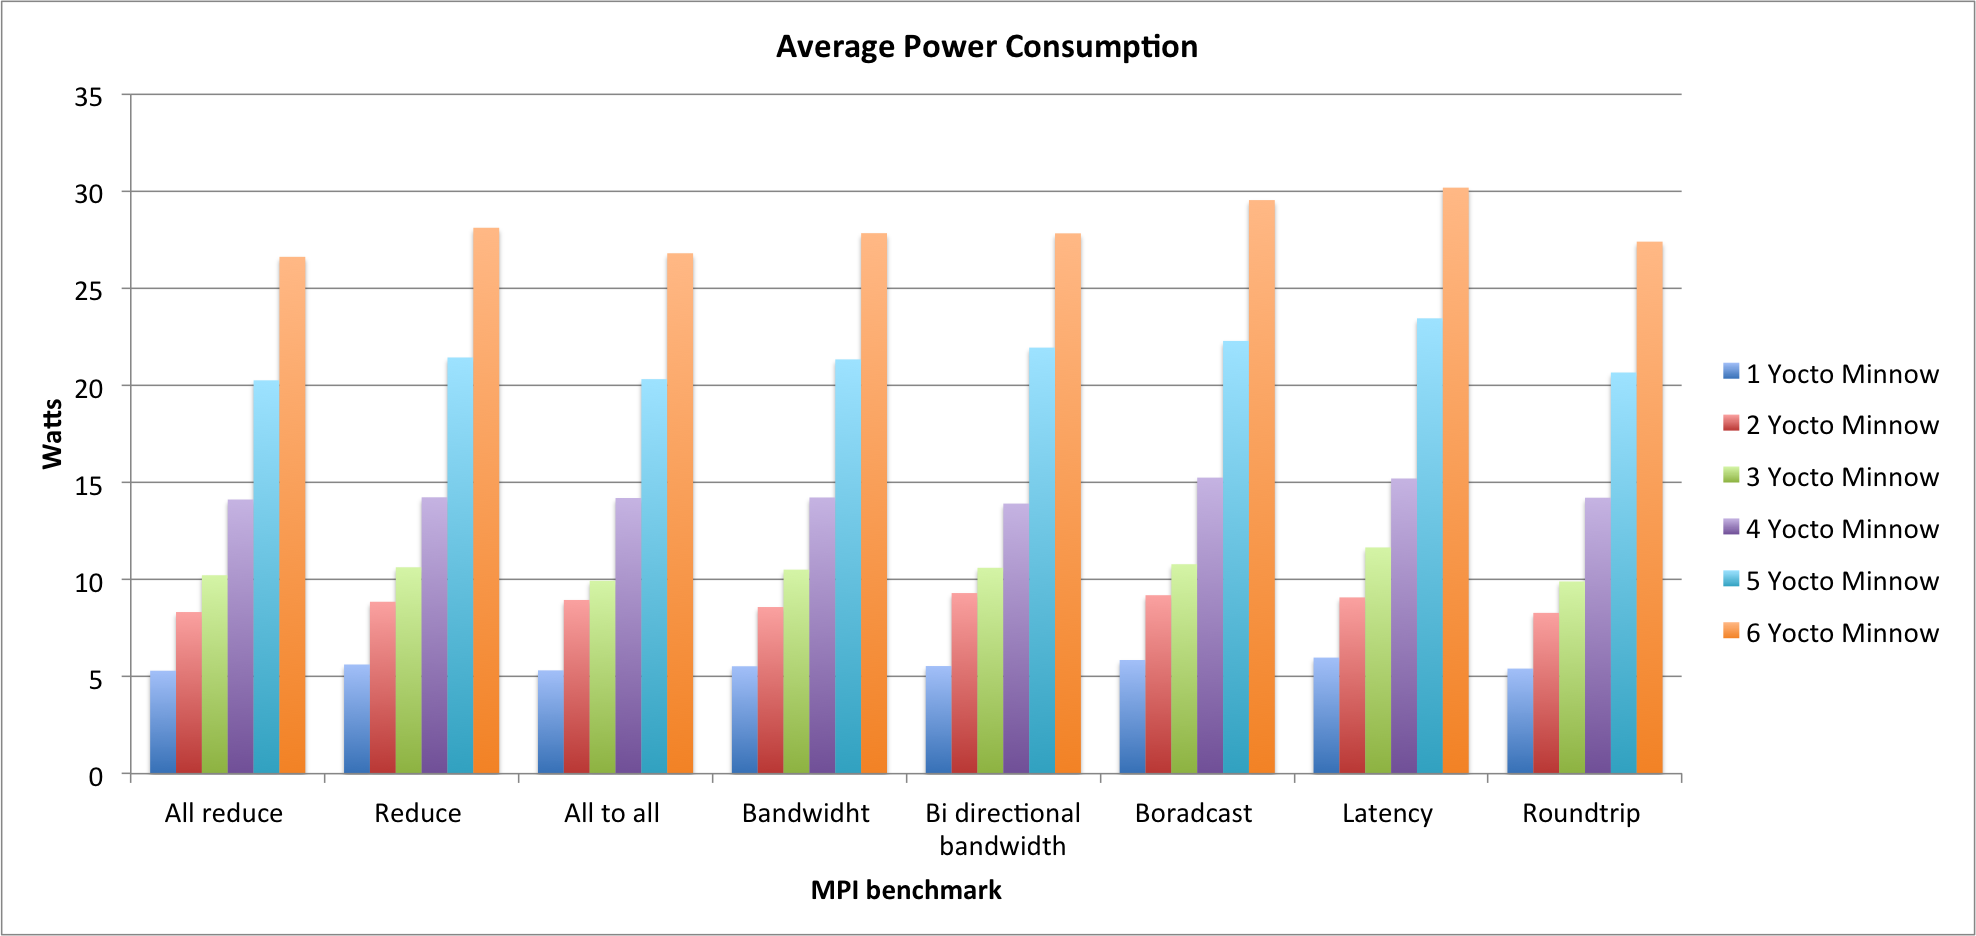
\includegraphics[width=0.75\textwidth]{images/power_average.png}
\caption{Average power management}
\label{power_average_minnow}
\end{figure}


The energy eficienty characterization of the systems can be described in the
following graphs: 

Number of platforms

\begin{figure}[H]
\centering
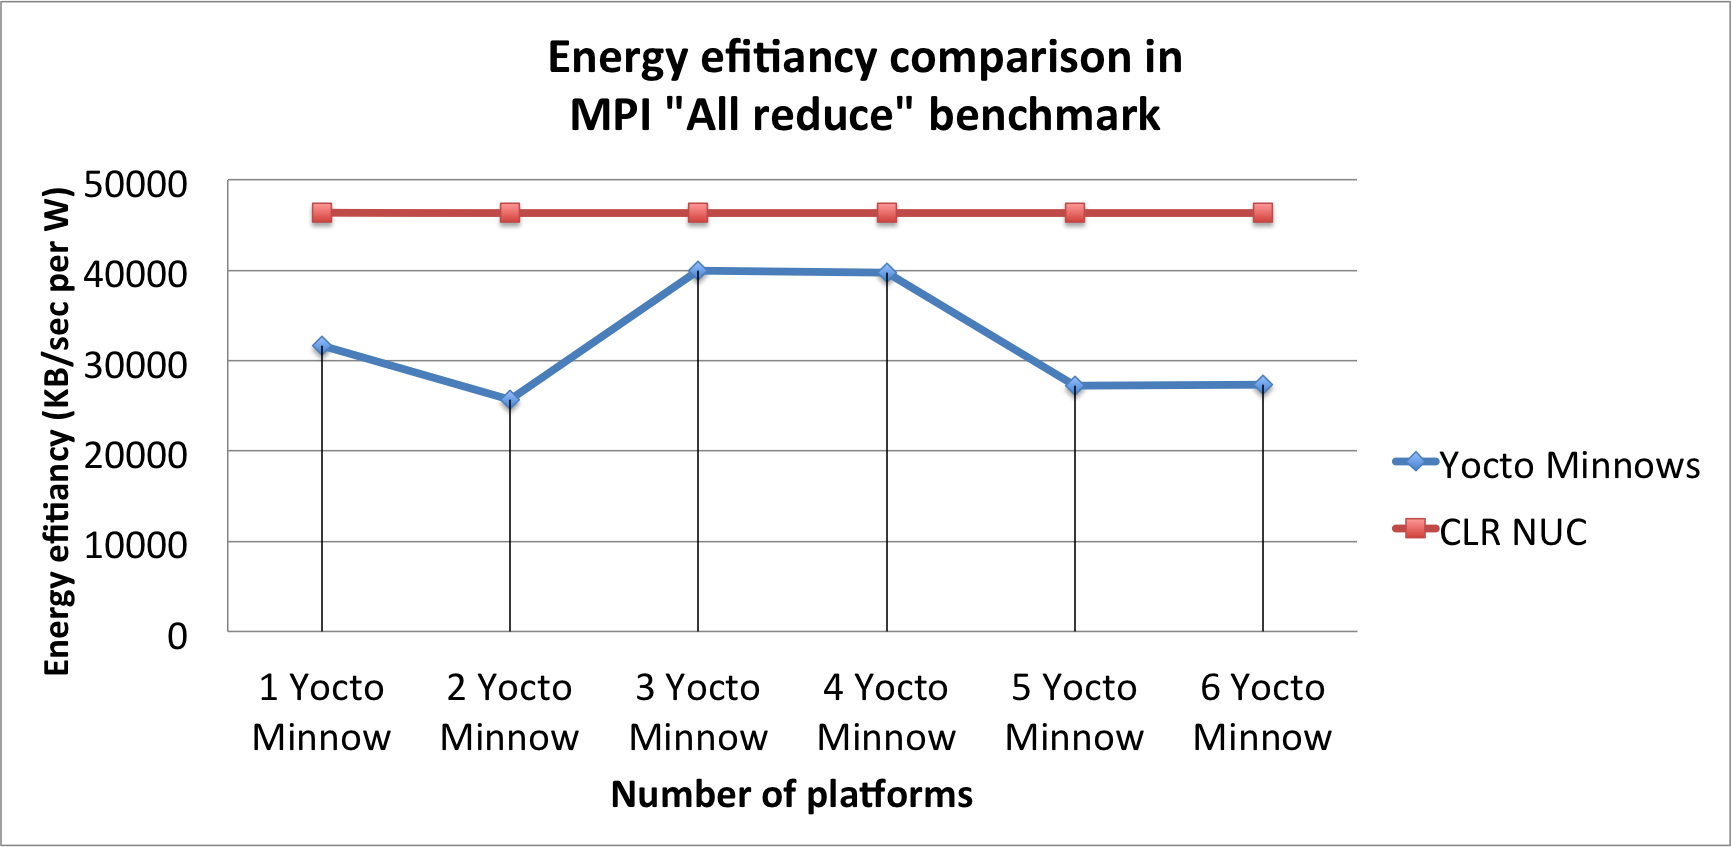
\includegraphics[width=0.75\textwidth]{images/energy_results/allreduce.png}
\caption{Energy efitiancy comparison in MPI "All reduce" benchmark (lower is
better)}
\label{all_reduce_energy}
\end{figure}


\begin{figure}[H]
\centering
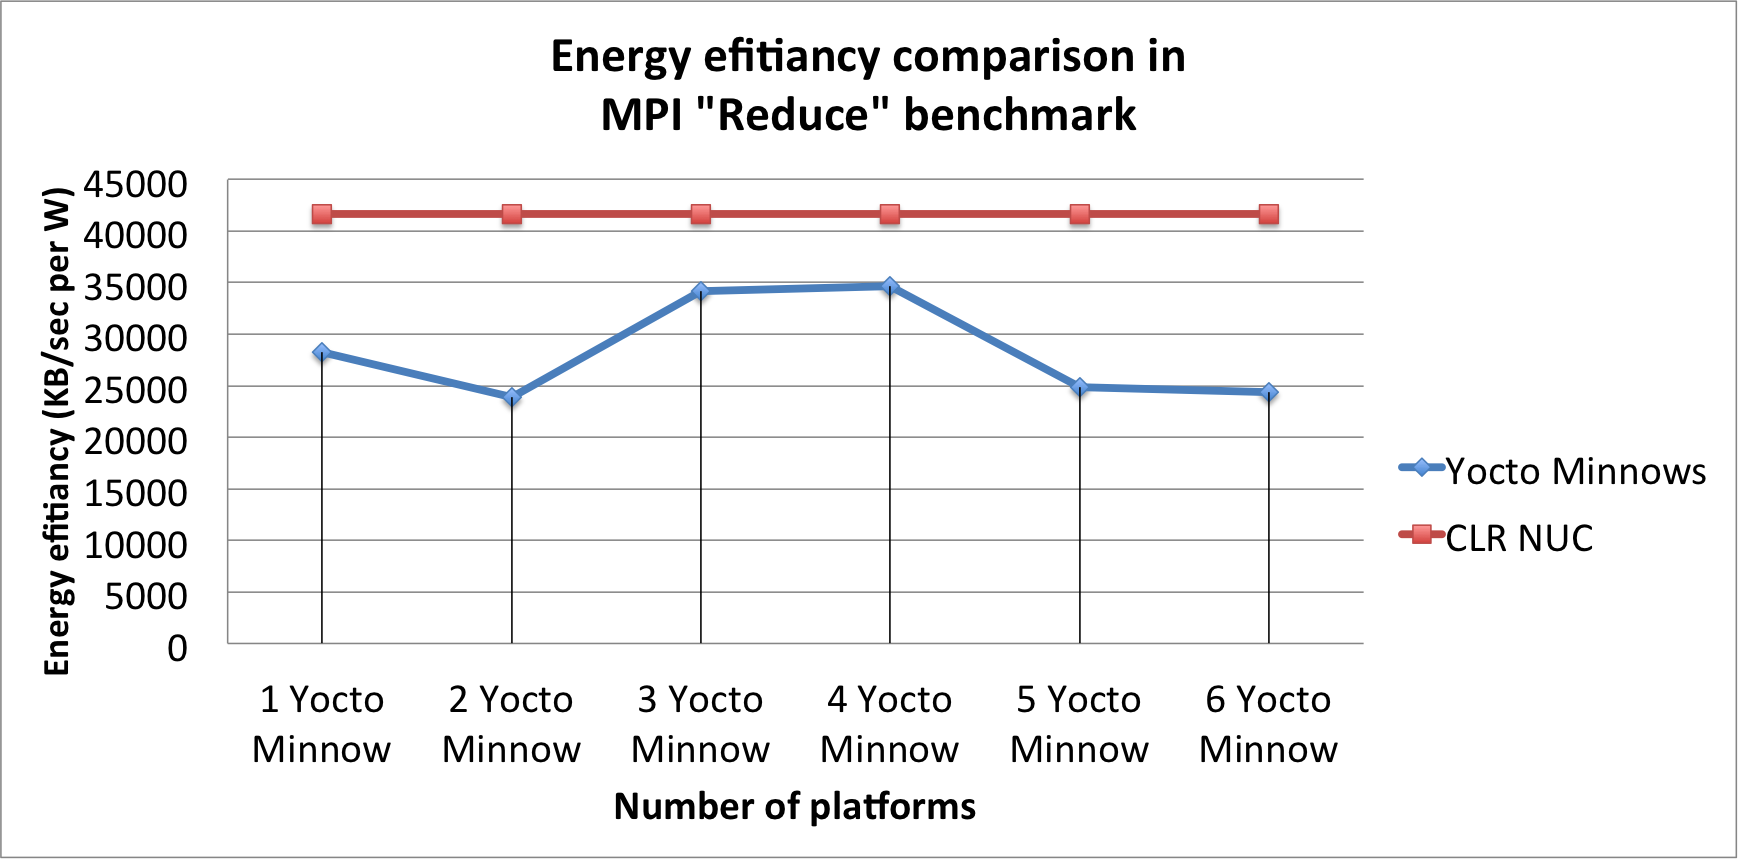
\includegraphics[width=0.75\textwidth]{images/energy_results/reduce.png}
\caption{Energy efitiancy comparison in MPI "Reduce" benchmark (lower is
better)}
\label{reduce_energy}
\end{figure}


\begin{figure}[H]
\centering
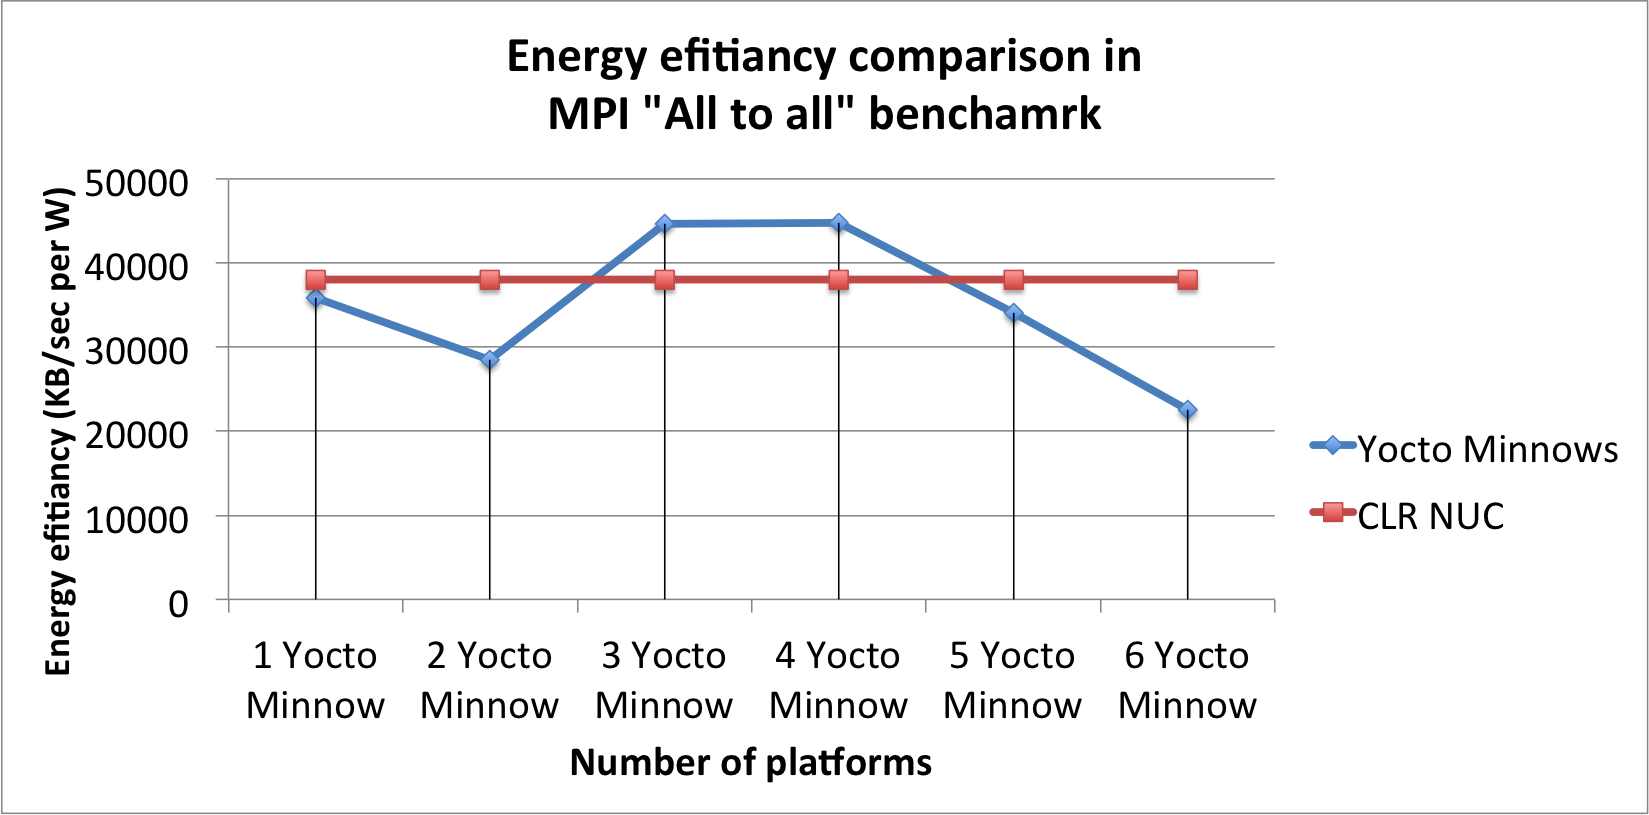
\includegraphics[width=0.75\textwidth]{images/energy_results/all_to_all.png}
\caption{Energy efitiancy comparison in MPI "All to all" benchmark (lower is
better)}
\label{alltoall_energy}
\end{figure}


\begin{figure}[H]
\centering
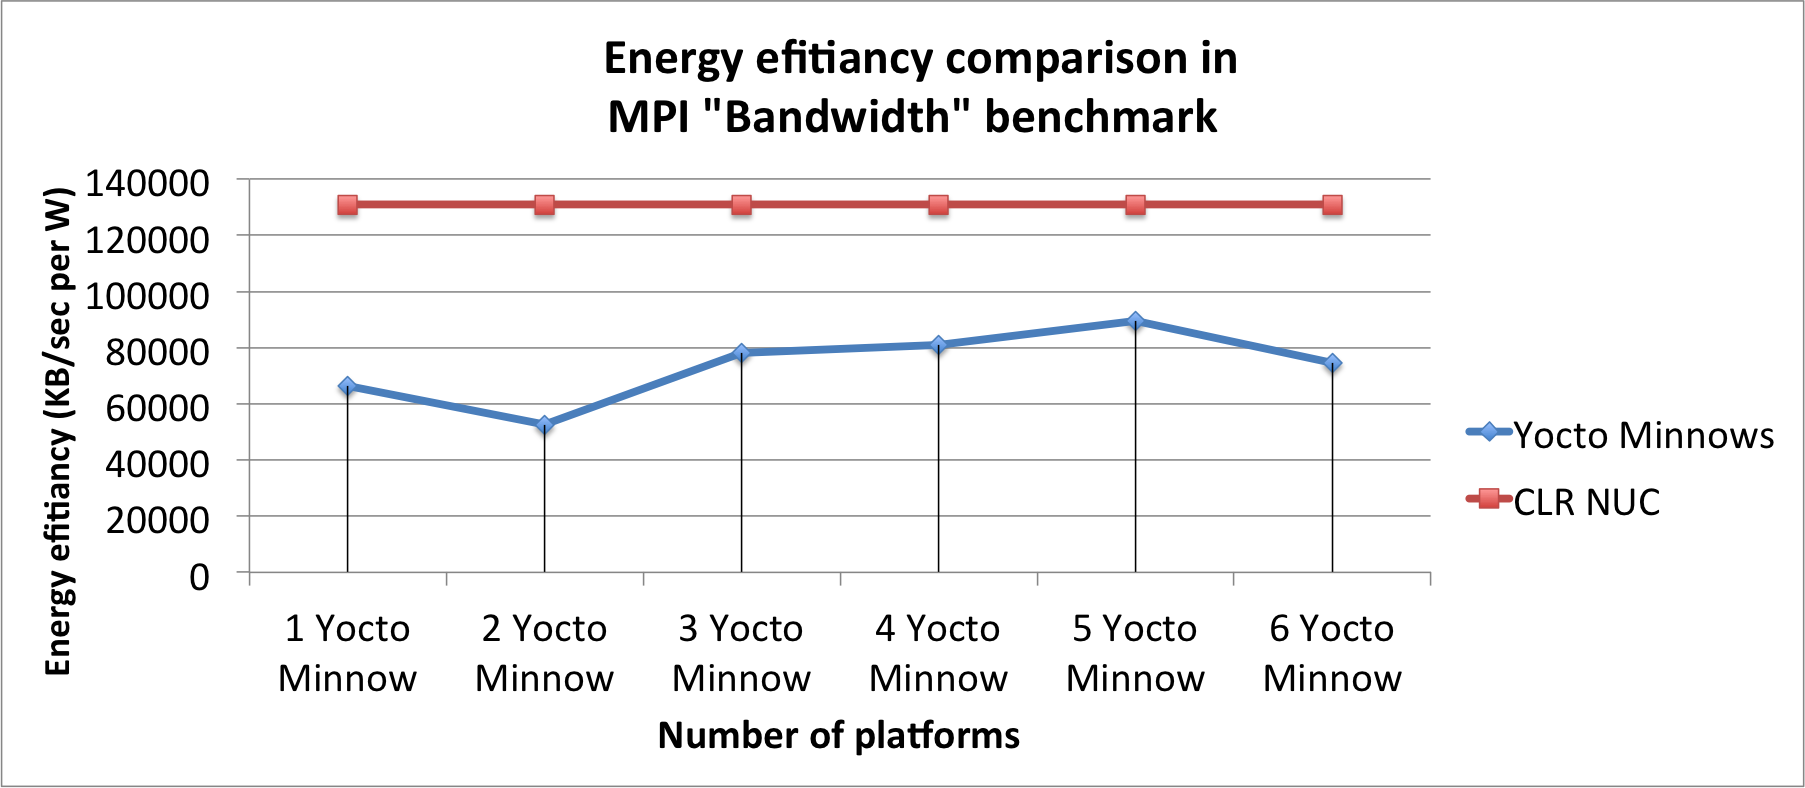
\includegraphics[width=0.75\textwidth]{images/energy_results/bandwidth.png}
\caption{Energy efitiancy comparison in MPI "Bandwidth" benchmark (lower is
better)}
\label{bandwidth_energy}
\end{figure}

\begin{figure}[H]
\centering
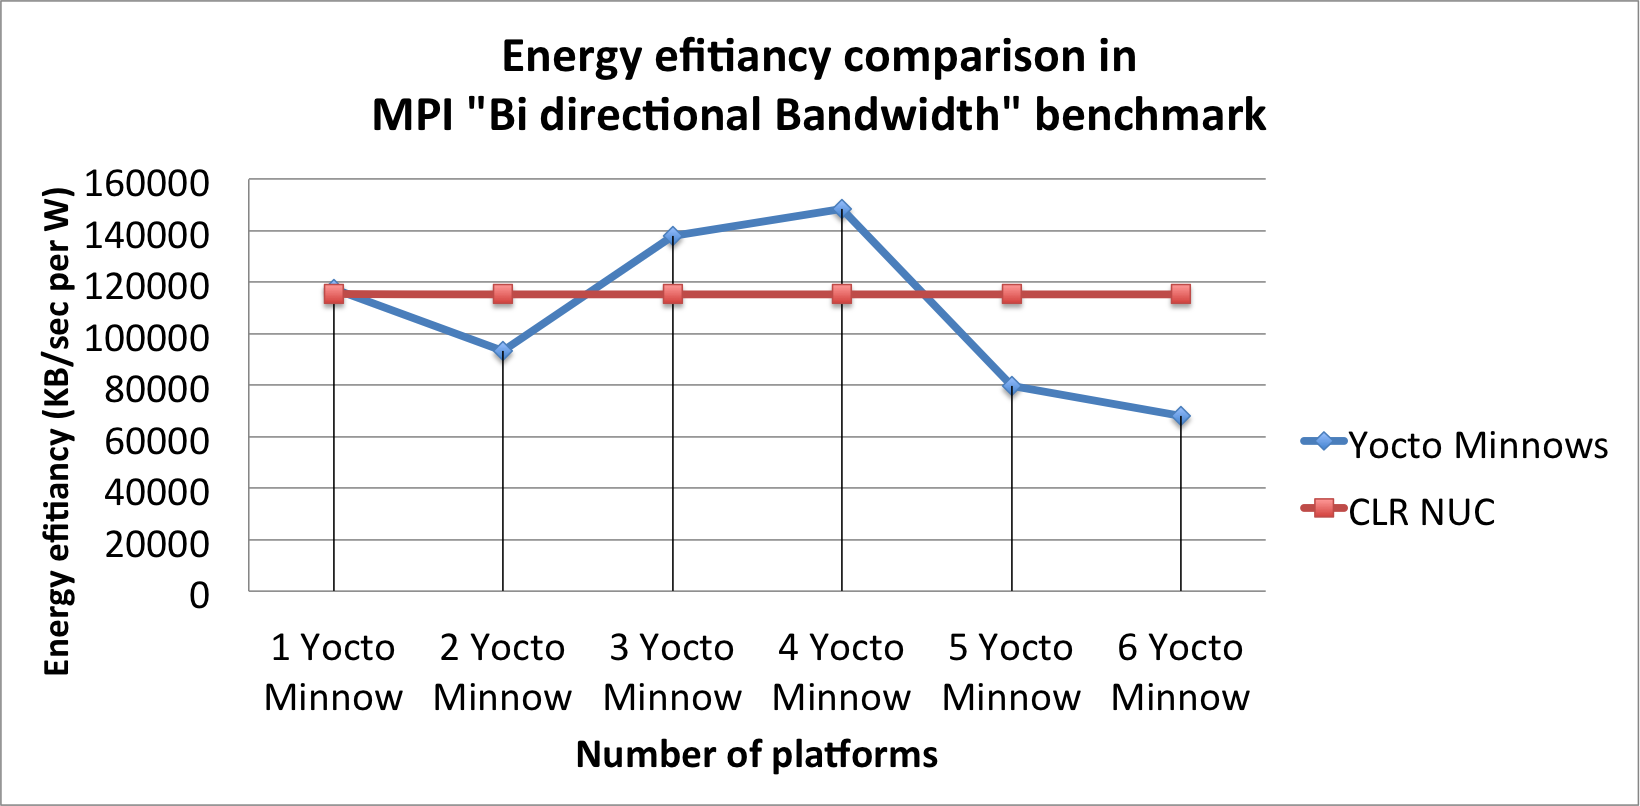
\includegraphics[width=0.75\textwidth]{images/energy_results/bibw.png}
\caption{Energy efitiancy comparison in MPI " Bi directional Bandwidth" benchmark (lower is
better)}
\label{bibw_energy}
\end{figure}


\begin{figure}[H]
\centering
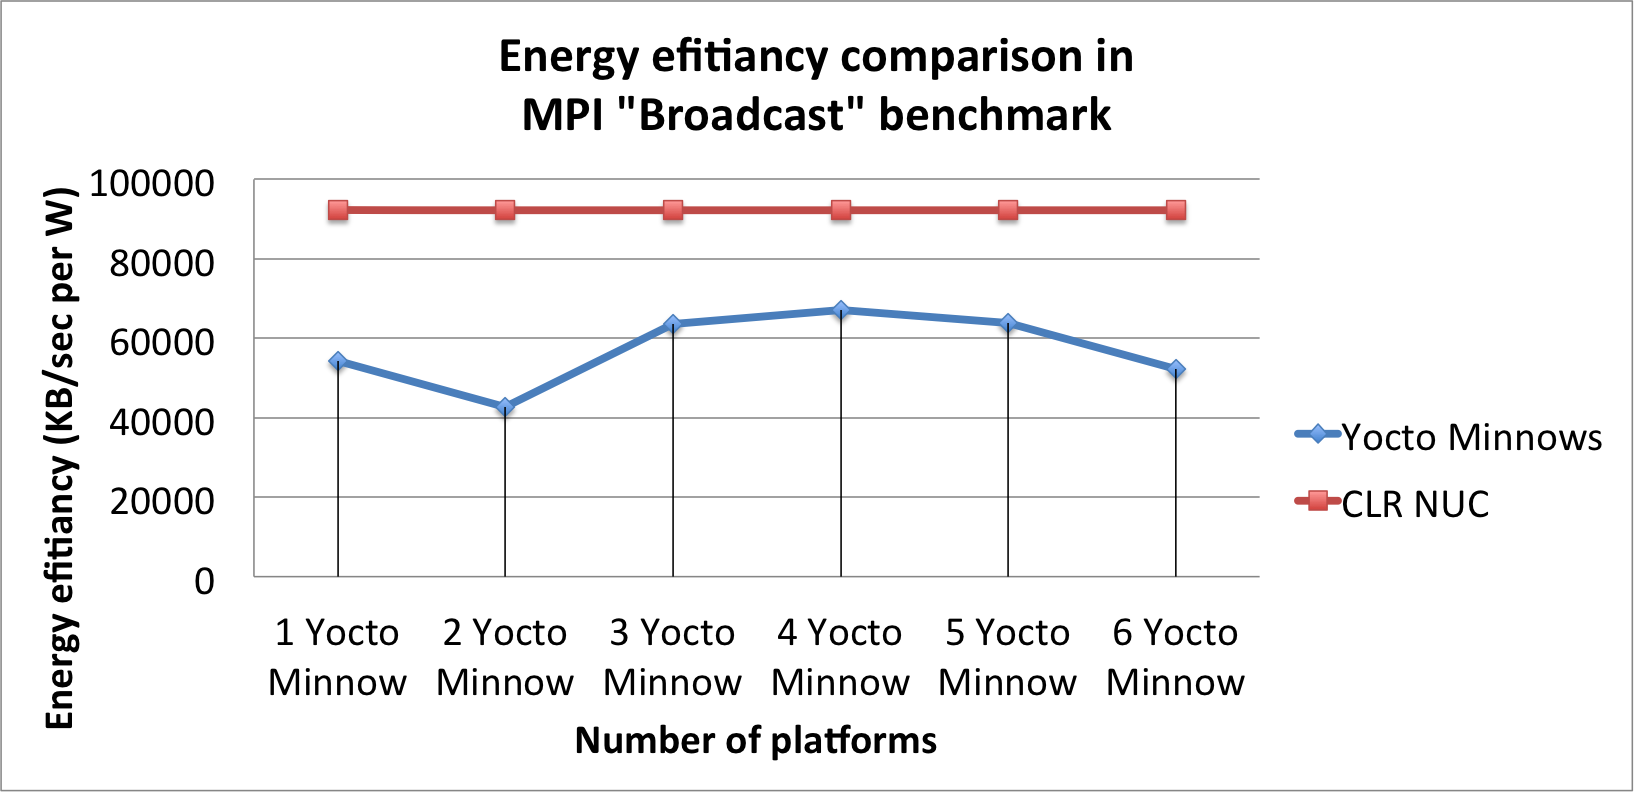
\includegraphics[width=0.75\textwidth]{images/energy_results/broadcast.png}
\caption{Energy efitiancy comparison in MPI " Broadcast Bandwidth" benchmark (lower is
better)}
\label{broadcast_energy}
\end{figure}


\section{Implement cluster of embedded systems for green house application}


\clearpage
